\documentclass[twoside]{book}

% Packages required by doxygen
\usepackage{fixltx2e}
\usepackage{calc}
\usepackage{doxygen}
\usepackage[export]{adjustbox} % also loads graphicx
\usepackage{graphicx}
\usepackage[utf8]{inputenc}
\usepackage{makeidx}
\usepackage{multicol}
\usepackage{multirow}
\PassOptionsToPackage{warn}{textcomp}
\usepackage{textcomp}
\usepackage[nointegrals]{wasysym}
\usepackage[table]{xcolor}

% Font selection
\usepackage[T1]{fontenc}
\usepackage[scaled=.90]{helvet}
\usepackage{courier}
\usepackage{amssymb}
\usepackage{sectsty}
\renewcommand{\familydefault}{\sfdefault}
\allsectionsfont{%
  \fontseries{bc}\selectfont%
  \color{darkgray}%
}
\renewcommand{\DoxyLabelFont}{%
  \fontseries{bc}\selectfont%
  \color{darkgray}%
}
\newcommand{\+}{\discretionary{\mbox{\scriptsize$\hookleftarrow$}}{}{}}

% Page & text layout
\usepackage{geometry}
\geometry{%
  a4paper,%
  top=2.5cm,%
  bottom=2.5cm,%
  left=2.5cm,%
  right=2.5cm%
}
\tolerance=750
\hfuzz=15pt
\hbadness=750
\setlength{\emergencystretch}{15pt}
\setlength{\parindent}{0cm}
\setlength{\parskip}{3ex plus 2ex minus 2ex}
\makeatletter
\renewcommand{\paragraph}{%
  \@startsection{paragraph}{4}{0ex}{-1.0ex}{1.0ex}{%
    \normalfont\normalsize\bfseries\SS@parafont%
  }%
}
\renewcommand{\subparagraph}{%
  \@startsection{subparagraph}{5}{0ex}{-1.0ex}{1.0ex}{%
    \normalfont\normalsize\bfseries\SS@subparafont%
  }%
}
\makeatother

% Headers & footers
\usepackage{fancyhdr}
\pagestyle{fancyplain}
\fancyhead[LE]{\fancyplain{}{\bfseries\thepage}}
\fancyhead[CE]{\fancyplain{}{}}
\fancyhead[RE]{\fancyplain{}{\bfseries\leftmark}}
\fancyhead[LO]{\fancyplain{}{\bfseries\rightmark}}
\fancyhead[CO]{\fancyplain{}{}}
\fancyhead[RO]{\fancyplain{}{\bfseries\thepage}}
\fancyfoot[LE]{\fancyplain{}{}}
\fancyfoot[CE]{\fancyplain{}{}}
\fancyfoot[RE]{\fancyplain{}{\bfseries\scriptsize Generated by Doxygen }}
\fancyfoot[LO]{\fancyplain{}{\bfseries\scriptsize Generated by Doxygen }}
\fancyfoot[CO]{\fancyplain{}{}}
\fancyfoot[RO]{\fancyplain{}{}}
\renewcommand{\footrulewidth}{0.4pt}
\renewcommand{\chaptermark}[1]{%
  \markboth{#1}{}%
}
\renewcommand{\sectionmark}[1]{%
  \markright{\thesection\ #1}%
}

% Indices & bibliography
\usepackage{natbib}
\usepackage[titles]{tocloft}
\setcounter{tocdepth}{3}
\setcounter{secnumdepth}{5}
\makeindex

% Hyperlinks (required, but should be loaded last)
\usepackage{ifpdf}
\ifpdf
  \usepackage[pdftex,pagebackref=true]{hyperref}
\else
  \usepackage[ps2pdf,pagebackref=true]{hyperref}
\fi
\hypersetup{%
  colorlinks=true,%
  linkcolor=blue,%
  citecolor=blue,%
  unicode%
}

% Custom commands
\newcommand{\clearemptydoublepage}{%
  \newpage{\pagestyle{empty}\cleardoublepage}%
}

\usepackage{caption}
\captionsetup{labelsep=space,justification=centering,font={bf},singlelinecheck=off,skip=4pt,position=top}

%===== C O N T E N T S =====

\begin{document}

% Titlepage & ToC
\hypersetup{pageanchor=false,
             bookmarksnumbered=true,
             pdfencoding=unicode
            }
\pagenumbering{roman}
\begin{titlepage}
\vspace*{7cm}
\begin{center}%
{\Large Behavior Path Planner }\\
\vspace*{1cm}
{\large Generated by Doxygen 1.8.11}\\
\end{center}
\end{titlepage}
\clearemptydoublepage
\tableofcontents
\clearemptydoublepage
\pagenumbering{arabic}
\hypersetup{pageanchor=true}

%--- Begin generated contents ---
\chapter{Namespace Index}
\section{Namespace List}
Here is a list of all namespaces with brief descriptions\+:\begin{DoxyCompactList}
\item\contentsline{section}{\hyperlink{namespacetk}{tk} }{\pageref{namespacetk}}{}
\end{DoxyCompactList}

\chapter{Hierarchical Index}
\section{Class Hierarchy}
This inheritance list is sorted roughly, but not completely, alphabetically\+:\begin{DoxyCompactList}
\item \contentsline{section}{Abstract\+Vehicle}{\pageref{classAbstractVehicle}}{}
\begin{DoxyCompactList}
\item \contentsline{section}{Ego\+Vehicle}{\pageref{classEgoVehicle}}{}
\item \contentsline{section}{Sensor\+Object}{\pageref{classSensorObject}}{}
\end{DoxyCompactList}
\item \contentsline{section}{Behavior\+Planner}{\pageref{classBehaviorPlanner}}{}
\item \contentsline{section}{Timer}{\pageref{classTimer}}{}
\item \contentsline{section}{Trajectory\+Planner}{\pageref{classTrajectoryPlanner}}{}
\item \contentsline{section}{Trajectory\+Planner\+W\+IP}{\pageref{classTrajectoryPlannerWIP}}{}
\end{DoxyCompactList}

\chapter{Class Index}
\section{Class List}
Here are the classes, structs, unions and interfaces with brief descriptions\+:\begin{DoxyCompactList}
\item\contentsline{section}{\hyperlink{classAbstractVehicle}{Abstract\+Vehicle} }{\pageref{classAbstractVehicle}}{}
\item\contentsline{section}{\hyperlink{classBehaviorPlanner}{Behavior\+Planner} }{\pageref{classBehaviorPlanner}}{}
\item\contentsline{section}{\hyperlink{classEgoVehicle}{Ego\+Vehicle} }{\pageref{classEgoVehicle}}{}
\item\contentsline{section}{\hyperlink{classSensorObject}{Sensor\+Object} }{\pageref{classSensorObject}}{}
\item\contentsline{section}{\hyperlink{classTimer}{Timer} }{\pageref{classTimer}}{}
\item\contentsline{section}{\hyperlink{classTrajectoryPlanner}{Trajectory\+Planner} }{\pageref{classTrajectoryPlanner}}{}
\item\contentsline{section}{\hyperlink{classTrajectoryPlannerWIP}{Trajectory\+Planner\+W\+IP} }{\pageref{classTrajectoryPlannerWIP}}{}
\end{DoxyCompactList}

\chapter{File Index}
\section{File List}
Here is a list of all files with brief descriptions\+:\begin{DoxyCompactList}
\item\contentsline{section}{src/\hyperlink{AbstractVehicle_8cpp}{Abstract\+Vehicle.\+cpp} }{\pageref{AbstractVehicle_8cpp}}{}
\item\contentsline{section}{src/\hyperlink{AbstractVehicle_8h}{Abstract\+Vehicle.\+h} }{\pageref{AbstractVehicle_8h}}{}
\item\contentsline{section}{src/\hyperlink{BehaviorPlanner_8cpp}{Behavior\+Planner.\+cpp} }{\pageref{BehaviorPlanner_8cpp}}{}
\item\contentsline{section}{src/\hyperlink{BehaviorPlanner_8h}{Behavior\+Planner.\+h} }{\pageref{BehaviorPlanner_8h}}{}
\item\contentsline{section}{src/\hyperlink{EgoVehicle_8cpp}{Ego\+Vehicle.\+cpp} }{\pageref{EgoVehicle_8cpp}}{}
\item\contentsline{section}{src/\hyperlink{EgoVehicle_8h}{Ego\+Vehicle.\+h} }{\pageref{EgoVehicle_8h}}{}
\item\contentsline{section}{src/\hyperlink{helper_8h}{helper.\+h} }{\pageref{helper_8h}}{}
\item\contentsline{section}{src/\hyperlink{main_8cpp}{main.\+cpp} }{\pageref{main_8cpp}}{}
\item\contentsline{section}{src/\hyperlink{SensorObject_8cpp}{Sensor\+Object.\+cpp} }{\pageref{SensorObject_8cpp}}{}
\item\contentsline{section}{src/\hyperlink{SensorObject_8h}{Sensor\+Object.\+h} }{\pageref{SensorObject_8h}}{}
\item\contentsline{section}{src/\hyperlink{spline_8h}{spline.\+h} }{\pageref{spline_8h}}{}
\item\contentsline{section}{src/\hyperlink{TrajectoryPlanner_8cpp}{Trajectory\+Planner.\+cpp} }{\pageref{TrajectoryPlanner_8cpp}}{}
\item\contentsline{section}{src/\hyperlink{TrajectoryPlanner_8h}{Trajectory\+Planner.\+h} }{\pageref{TrajectoryPlanner_8h}}{}
\item\contentsline{section}{src/\hyperlink{TrajectoryPlannerWIP_8cpp}{Trajectory\+Planner\+W\+I\+P.\+cpp} }{\pageref{TrajectoryPlannerWIP_8cpp}}{}
\item\contentsline{section}{src/\hyperlink{TrajectoryPlannerWIP_8h}{Trajectory\+Planner\+W\+I\+P.\+h} }{\pageref{TrajectoryPlannerWIP_8h}}{}
\end{DoxyCompactList}

\chapter{Namespace Documentation}
\hypertarget{namespacetk}{}\section{tk Namespace Reference}
\label{namespacetk}\index{tk@{tk}}

\chapter{Class Documentation}
\hypertarget{classAbstractVehicle}{}\section{Abstract\+Vehicle Class Reference}
\label{classAbstractVehicle}\index{Abstract\+Vehicle@{Abstract\+Vehicle}}


{\ttfamily \#include $<$Abstract\+Vehicle.\+h$>$}



Inheritance diagram for Abstract\+Vehicle\+:\nopagebreak
\begin{figure}[H]
\begin{center}
\leavevmode
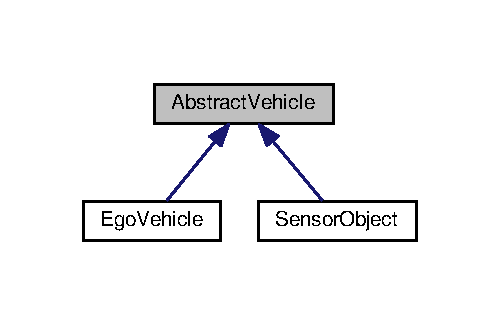
\includegraphics[width=240pt]{classAbstractVehicle__inherit__graph}
\end{center}
\end{figure}
\subsection*{Public Member Functions}
\begin{DoxyCompactItemize}
\item 
virtual double \hyperlink{classAbstractVehicle_a17c193d56e1da24a1008ae52859d31c7}{get\+Speed} ()=0
\item 
virtual double \hyperlink{classAbstractVehicle_abe9a9f5e2290fdf4207ac0206b9e97a3}{get\+Speed\+\_\+x} ()=0
\item 
virtual double \hyperlink{classAbstractVehicle_a90e6e4299070bace1acfd8d79bf78c95}{get\+Speed\+\_\+y} ()=0
\item 
virtual string \hyperlink{classAbstractVehicle_ada311ec475179ba776966f7e3ddcb91a}{display} ()=0
\item 
virtual void \hyperlink{classAbstractVehicle_a004b43b4a4d02ca6122ed8862c672de3}{update} (\hyperlink{main_8cpp_ab701e3ac61a85b337ec5c1abaad6742d}{json} j)=0
\item 
virtual vector$<$ double $>$ \hyperlink{classAbstractVehicle_a3c84d6970c9461bfafd76cf48d6bece0}{get\+Prediction} (int second)=0
\item 
int \hyperlink{classAbstractVehicle_aad5abe9ab0ba30d7a1e217408e7e9baa}{get\+Lane} ()
\begin{DoxyCompactList}\small\item\em get current lane number from vehicle \end{DoxyCompactList}\item 
double \hyperlink{classAbstractVehicle_a54d4973b14dbd842ec68fdce2b5950b8}{get\+Frenet\+\_\+s} ()
\item 
double \hyperlink{classAbstractVehicle_a2551fc01117e71f4a1d9c799f2ea2875}{get\+Frenet\+\_\+d} ()
\item 
double \hyperlink{classAbstractVehicle_a68789bdcd4abe63bde21ea2587a2ca0a}{get\+Cartesian\+\_\+x} ()
\item 
double \hyperlink{classAbstractVehicle_ab3415d624ff40a27fd709bd87560d2ac}{get\+Cartesian\+\_\+y} ()
\item 
double \hyperlink{classAbstractVehicle_ab334fb8d15fd2ea52abd255924bb4c15}{get\+ID} ()
\item 
virtual void \hyperlink{classAbstractVehicle_a631115b44756050ccf2a7fe975787035}{calculate\+Predictions} (int prediction\+Horizon)=0
\end{DoxyCompactItemize}
\subsection*{Protected Attributes}
\begin{DoxyCompactItemize}
\item 
double \hyperlink{classAbstractVehicle_ae714379f009c459ec3b3856140204c8e}{id}
\item 
double \hyperlink{classAbstractVehicle_a8fe56b85f2acffbbb5e451b99f4883b4}{frenet\+\_\+s}
\item 
double \hyperlink{classAbstractVehicle_a6a98d1a83288b4c7c7d70b09f606e648}{frenet\+\_\+d}
\item 
double \hyperlink{classAbstractVehicle_a4e60d7e6e2d55940227bd6e31e3bb5a6}{cartesian\+\_\+x}
\item 
double \hyperlink{classAbstractVehicle_a16bb1778276fb773f1bfa0fbb855eb6d}{cartesian\+\_\+y}
\item 
int \hyperlink{classAbstractVehicle_adb32774724d498cfcdf2309e0a189b6e}{last\+Lane}
\item 
int \hyperlink{classAbstractVehicle_aa0a52d60f51e34c045db63ecc4a96f98}{current\+Lane}
\item 
std\+::vector$<$ double $>$ \hyperlink{classAbstractVehicle_ac9370b8bc9863b02dbc17f0d3429ce2d}{last\+\_\+frenet\+\_\+d}
\item 
std\+::vector$<$ double $>$ \hyperlink{classAbstractVehicle_a087956b0de86efa9434da992fdb2d27d}{last\+\_\+frenet\+\_\+s}
\item 
int \hyperlink{classAbstractVehicle_a5cf60337402a5d6457229e186a403dc5}{history\+Length} = 10
\item 
int \hyperlink{classAbstractVehicle_ae24b37395a3fa832a82b6460a127378b}{prediction\+Horizon\+In\+Seconds} = 10
\item 
std\+::vector$<$ std\+::vector$<$ double $>$ $>$ \hyperlink{classAbstractVehicle_a72ef849b0da369f2eb74ca091b1e00b7}{predictions}
\end{DoxyCompactItemize}


\subsection{Detailed Description}
Abstract class for Vehicles\+: ego and other 

\subsection{Member Function Documentation}
\index{Abstract\+Vehicle@{Abstract\+Vehicle}!calculate\+Predictions@{calculate\+Predictions}}
\index{calculate\+Predictions@{calculate\+Predictions}!Abstract\+Vehicle@{Abstract\+Vehicle}}
\subsubsection[{\texorpdfstring{calculate\+Predictions(int prediction\+Horizon)=0}{calculatePredictions(int predictionHorizon)=0}}]{\setlength{\rightskip}{0pt plus 5cm}virtual void Abstract\+Vehicle\+::calculate\+Predictions (
\begin{DoxyParamCaption}
\item[{int}]{prediction\+Horizon}
\end{DoxyParamCaption}
)\hspace{0.3cm}{\ttfamily [pure virtual]}}\hypertarget{classAbstractVehicle_a631115b44756050ccf2a7fe975787035}{}\label{classAbstractVehicle_a631115b44756050ccf2a7fe975787035}


Implemented in \hyperlink{classEgoVehicle_ae0b5afee444e02d3211d1bc0c6524bbe}{Ego\+Vehicle}, and \hyperlink{classSensorObject_a6787ced615e75d519842ab2e893048ca}{Sensor\+Object}.

\index{Abstract\+Vehicle@{Abstract\+Vehicle}!display@{display}}
\index{display@{display}!Abstract\+Vehicle@{Abstract\+Vehicle}}
\subsubsection[{\texorpdfstring{display()=0}{display()=0}}]{\setlength{\rightskip}{0pt plus 5cm}virtual string Abstract\+Vehicle\+::display (
\begin{DoxyParamCaption}
{}
\end{DoxyParamCaption}
)\hspace{0.3cm}{\ttfamily [pure virtual]}}\hypertarget{classAbstractVehicle_ada311ec475179ba776966f7e3ddcb91a}{}\label{classAbstractVehicle_ada311ec475179ba776966f7e3ddcb91a}


Implemented in \hyperlink{classEgoVehicle_a68e3c46400e34d4f805fcc392ecd5563}{Ego\+Vehicle}, and \hyperlink{classSensorObject_adaa7350730c3c627f0f215c251386cb7}{Sensor\+Object}.

\index{Abstract\+Vehicle@{Abstract\+Vehicle}!get\+Cartesian\+\_\+x@{get\+Cartesian\+\_\+x}}
\index{get\+Cartesian\+\_\+x@{get\+Cartesian\+\_\+x}!Abstract\+Vehicle@{Abstract\+Vehicle}}
\subsubsection[{\texorpdfstring{get\+Cartesian\+\_\+x()}{getCartesian_x()}}]{\setlength{\rightskip}{0pt plus 5cm}double Abstract\+Vehicle\+::get\+Cartesian\+\_\+x (
\begin{DoxyParamCaption}
{}
\end{DoxyParamCaption}
)\hspace{0.3cm}{\ttfamily [inline]}}\hypertarget{classAbstractVehicle_a68789bdcd4abe63bde21ea2587a2ca0a}{}\label{classAbstractVehicle_a68789bdcd4abe63bde21ea2587a2ca0a}
\index{Abstract\+Vehicle@{Abstract\+Vehicle}!get\+Cartesian\+\_\+y@{get\+Cartesian\+\_\+y}}
\index{get\+Cartesian\+\_\+y@{get\+Cartesian\+\_\+y}!Abstract\+Vehicle@{Abstract\+Vehicle}}
\subsubsection[{\texorpdfstring{get\+Cartesian\+\_\+y()}{getCartesian_y()}}]{\setlength{\rightskip}{0pt plus 5cm}double Abstract\+Vehicle\+::get\+Cartesian\+\_\+y (
\begin{DoxyParamCaption}
{}
\end{DoxyParamCaption}
)\hspace{0.3cm}{\ttfamily [inline]}}\hypertarget{classAbstractVehicle_ab3415d624ff40a27fd709bd87560d2ac}{}\label{classAbstractVehicle_ab3415d624ff40a27fd709bd87560d2ac}
\index{Abstract\+Vehicle@{Abstract\+Vehicle}!get\+Frenet\+\_\+d@{get\+Frenet\+\_\+d}}
\index{get\+Frenet\+\_\+d@{get\+Frenet\+\_\+d}!Abstract\+Vehicle@{Abstract\+Vehicle}}
\subsubsection[{\texorpdfstring{get\+Frenet\+\_\+d()}{getFrenet_d()}}]{\setlength{\rightskip}{0pt plus 5cm}double Abstract\+Vehicle\+::get\+Frenet\+\_\+d (
\begin{DoxyParamCaption}
{}
\end{DoxyParamCaption}
)\hspace{0.3cm}{\ttfamily [inline]}}\hypertarget{classAbstractVehicle_a2551fc01117e71f4a1d9c799f2ea2875}{}\label{classAbstractVehicle_a2551fc01117e71f4a1d9c799f2ea2875}
\index{Abstract\+Vehicle@{Abstract\+Vehicle}!get\+Frenet\+\_\+s@{get\+Frenet\+\_\+s}}
\index{get\+Frenet\+\_\+s@{get\+Frenet\+\_\+s}!Abstract\+Vehicle@{Abstract\+Vehicle}}
\subsubsection[{\texorpdfstring{get\+Frenet\+\_\+s()}{getFrenet_s()}}]{\setlength{\rightskip}{0pt plus 5cm}double Abstract\+Vehicle\+::get\+Frenet\+\_\+s (
\begin{DoxyParamCaption}
{}
\end{DoxyParamCaption}
)\hspace{0.3cm}{\ttfamily [inline]}}\hypertarget{classAbstractVehicle_a54d4973b14dbd842ec68fdce2b5950b8}{}\label{classAbstractVehicle_a54d4973b14dbd842ec68fdce2b5950b8}
\index{Abstract\+Vehicle@{Abstract\+Vehicle}!get\+ID@{get\+ID}}
\index{get\+ID@{get\+ID}!Abstract\+Vehicle@{Abstract\+Vehicle}}
\subsubsection[{\texorpdfstring{get\+I\+D()}{getID()}}]{\setlength{\rightskip}{0pt plus 5cm}double Abstract\+Vehicle\+::get\+ID (
\begin{DoxyParamCaption}
{}
\end{DoxyParamCaption}
)\hspace{0.3cm}{\ttfamily [inline]}}\hypertarget{classAbstractVehicle_ab334fb8d15fd2ea52abd255924bb4c15}{}\label{classAbstractVehicle_ab334fb8d15fd2ea52abd255924bb4c15}


Here is the call graph for this function\+:\nopagebreak
\begin{figure}[H]
\begin{center}
\leavevmode
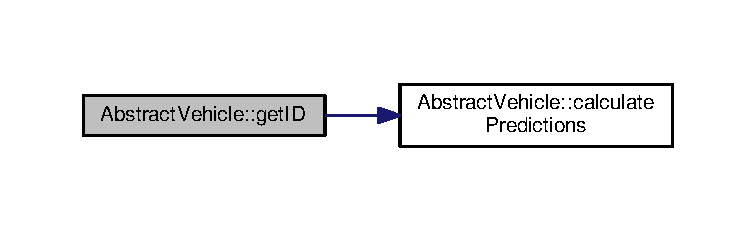
\includegraphics[width=350pt]{classAbstractVehicle_ab334fb8d15fd2ea52abd255924bb4c15_cgraph}
\end{center}
\end{figure}


\index{Abstract\+Vehicle@{Abstract\+Vehicle}!get\+Lane@{get\+Lane}}
\index{get\+Lane@{get\+Lane}!Abstract\+Vehicle@{Abstract\+Vehicle}}
\subsubsection[{\texorpdfstring{get\+Lane()}{getLane()}}]{\setlength{\rightskip}{0pt plus 5cm}int Abstract\+Vehicle\+::get\+Lane (
\begin{DoxyParamCaption}
{}
\end{DoxyParamCaption}
)}\hypertarget{classAbstractVehicle_aad5abe9ab0ba30d7a1e217408e7e9baa}{}\label{classAbstractVehicle_aad5abe9ab0ba30d7a1e217408e7e9baa}


get current lane number from vehicle 

\begin{DoxyReturn}{Returns}
int lane number 
\end{DoxyReturn}
\begin{DoxyNote}{Note}

\begin{DoxyItemize}
\item lane width is 4 meters
\item left lane = lane 0
\item middle lane = lane 1
\item right lane = lane 2
\end{DoxyItemize}
\end{DoxyNote}
\index{Abstract\+Vehicle@{Abstract\+Vehicle}!get\+Prediction@{get\+Prediction}}
\index{get\+Prediction@{get\+Prediction}!Abstract\+Vehicle@{Abstract\+Vehicle}}
\subsubsection[{\texorpdfstring{get\+Prediction(int second)=0}{getPrediction(int second)=0}}]{\setlength{\rightskip}{0pt plus 5cm}virtual vector$<$double$>$ Abstract\+Vehicle\+::get\+Prediction (
\begin{DoxyParamCaption}
\item[{int}]{second}
\end{DoxyParamCaption}
)\hspace{0.3cm}{\ttfamily [pure virtual]}}\hypertarget{classAbstractVehicle_a3c84d6970c9461bfafd76cf48d6bece0}{}\label{classAbstractVehicle_a3c84d6970c9461bfafd76cf48d6bece0}


Implemented in \hyperlink{classEgoVehicle_af44e6b8bb8af7410ea404b8939507c93}{Ego\+Vehicle}, and \hyperlink{classSensorObject_a49714af72f563ce1114c9f43e95d7af8}{Sensor\+Object}.

\index{Abstract\+Vehicle@{Abstract\+Vehicle}!get\+Speed@{get\+Speed}}
\index{get\+Speed@{get\+Speed}!Abstract\+Vehicle@{Abstract\+Vehicle}}
\subsubsection[{\texorpdfstring{get\+Speed()=0}{getSpeed()=0}}]{\setlength{\rightskip}{0pt plus 5cm}virtual double Abstract\+Vehicle\+::get\+Speed (
\begin{DoxyParamCaption}
{}
\end{DoxyParamCaption}
)\hspace{0.3cm}{\ttfamily [pure virtual]}}\hypertarget{classAbstractVehicle_a17c193d56e1da24a1008ae52859d31c7}{}\label{classAbstractVehicle_a17c193d56e1da24a1008ae52859d31c7}


Implemented in \hyperlink{classEgoVehicle_a8062f2bbb14f1bd787921cd83d4e5475}{Ego\+Vehicle}, and \hyperlink{classSensorObject_ab3e8516fb8273082efbc873266667486}{Sensor\+Object}.

\index{Abstract\+Vehicle@{Abstract\+Vehicle}!get\+Speed\+\_\+x@{get\+Speed\+\_\+x}}
\index{get\+Speed\+\_\+x@{get\+Speed\+\_\+x}!Abstract\+Vehicle@{Abstract\+Vehicle}}
\subsubsection[{\texorpdfstring{get\+Speed\+\_\+x()=0}{getSpeed_x()=0}}]{\setlength{\rightskip}{0pt plus 5cm}virtual double Abstract\+Vehicle\+::get\+Speed\+\_\+x (
\begin{DoxyParamCaption}
{}
\end{DoxyParamCaption}
)\hspace{0.3cm}{\ttfamily [pure virtual]}}\hypertarget{classAbstractVehicle_abe9a9f5e2290fdf4207ac0206b9e97a3}{}\label{classAbstractVehicle_abe9a9f5e2290fdf4207ac0206b9e97a3}


Implemented in \hyperlink{classEgoVehicle_a692add014c4846c554c4d08e170c140a}{Ego\+Vehicle}, and \hyperlink{classSensorObject_abcd7baf59194b7fef7d0ec75eb880123}{Sensor\+Object}.

\index{Abstract\+Vehicle@{Abstract\+Vehicle}!get\+Speed\+\_\+y@{get\+Speed\+\_\+y}}
\index{get\+Speed\+\_\+y@{get\+Speed\+\_\+y}!Abstract\+Vehicle@{Abstract\+Vehicle}}
\subsubsection[{\texorpdfstring{get\+Speed\+\_\+y()=0}{getSpeed_y()=0}}]{\setlength{\rightskip}{0pt plus 5cm}virtual double Abstract\+Vehicle\+::get\+Speed\+\_\+y (
\begin{DoxyParamCaption}
{}
\end{DoxyParamCaption}
)\hspace{0.3cm}{\ttfamily [pure virtual]}}\hypertarget{classAbstractVehicle_a90e6e4299070bace1acfd8d79bf78c95}{}\label{classAbstractVehicle_a90e6e4299070bace1acfd8d79bf78c95}


Implemented in \hyperlink{classEgoVehicle_a88d4bc1d06c685f060d8e628452173fb}{Ego\+Vehicle}, and \hyperlink{classSensorObject_a0fcc2d7351b630b61fbd5395ac568bc4}{Sensor\+Object}.

\index{Abstract\+Vehicle@{Abstract\+Vehicle}!update@{update}}
\index{update@{update}!Abstract\+Vehicle@{Abstract\+Vehicle}}
\subsubsection[{\texorpdfstring{update(json j)=0}{update(json j)=0}}]{\setlength{\rightskip}{0pt plus 5cm}virtual void Abstract\+Vehicle\+::update (
\begin{DoxyParamCaption}
\item[{{\bf json}}]{j}
\end{DoxyParamCaption}
)\hspace{0.3cm}{\ttfamily [pure virtual]}}\hypertarget{classAbstractVehicle_a004b43b4a4d02ca6122ed8862c672de3}{}\label{classAbstractVehicle_a004b43b4a4d02ca6122ed8862c672de3}


Implemented in \hyperlink{classEgoVehicle_ae189735224d6a6bb46f6170321c128dc}{Ego\+Vehicle}, and \hyperlink{classSensorObject_a4d0023c0d36c15df10aade6ec224cc56}{Sensor\+Object}.



\subsection{Member Data Documentation}
\index{Abstract\+Vehicle@{Abstract\+Vehicle}!cartesian\+\_\+x@{cartesian\+\_\+x}}
\index{cartesian\+\_\+x@{cartesian\+\_\+x}!Abstract\+Vehicle@{Abstract\+Vehicle}}
\subsubsection[{\texorpdfstring{cartesian\+\_\+x}{cartesian_x}}]{\setlength{\rightskip}{0pt plus 5cm}double Abstract\+Vehicle\+::cartesian\+\_\+x\hspace{0.3cm}{\ttfamily [protected]}}\hypertarget{classAbstractVehicle_a4e60d7e6e2d55940227bd6e31e3bb5a6}{}\label{classAbstractVehicle_a4e60d7e6e2d55940227bd6e31e3bb5a6}
x-\/value of vehicle \index{Abstract\+Vehicle@{Abstract\+Vehicle}!cartesian\+\_\+y@{cartesian\+\_\+y}}
\index{cartesian\+\_\+y@{cartesian\+\_\+y}!Abstract\+Vehicle@{Abstract\+Vehicle}}
\subsubsection[{\texorpdfstring{cartesian\+\_\+y}{cartesian_y}}]{\setlength{\rightskip}{0pt plus 5cm}double Abstract\+Vehicle\+::cartesian\+\_\+y\hspace{0.3cm}{\ttfamily [protected]}}\hypertarget{classAbstractVehicle_a16bb1778276fb773f1bfa0fbb855eb6d}{}\label{classAbstractVehicle_a16bb1778276fb773f1bfa0fbb855eb6d}
y-\/value of vehicle \index{Abstract\+Vehicle@{Abstract\+Vehicle}!current\+Lane@{current\+Lane}}
\index{current\+Lane@{current\+Lane}!Abstract\+Vehicle@{Abstract\+Vehicle}}
\subsubsection[{\texorpdfstring{current\+Lane}{currentLane}}]{\setlength{\rightskip}{0pt plus 5cm}int Abstract\+Vehicle\+::current\+Lane\hspace{0.3cm}{\ttfamily [protected]}}\hypertarget{classAbstractVehicle_aa0a52d60f51e34c045db63ecc4a96f98}{}\label{classAbstractVehicle_aa0a52d60f51e34c045db63ecc4a96f98}
current lane before \index{Abstract\+Vehicle@{Abstract\+Vehicle}!frenet\+\_\+d@{frenet\+\_\+d}}
\index{frenet\+\_\+d@{frenet\+\_\+d}!Abstract\+Vehicle@{Abstract\+Vehicle}}
\subsubsection[{\texorpdfstring{frenet\+\_\+d}{frenet_d}}]{\setlength{\rightskip}{0pt plus 5cm}double Abstract\+Vehicle\+::frenet\+\_\+d\hspace{0.3cm}{\ttfamily [protected]}}\hypertarget{classAbstractVehicle_a6a98d1a83288b4c7c7d70b09f606e648}{}\label{classAbstractVehicle_a6a98d1a83288b4c7c7d70b09f606e648}
d-\/frenet value of vehicle \index{Abstract\+Vehicle@{Abstract\+Vehicle}!frenet\+\_\+s@{frenet\+\_\+s}}
\index{frenet\+\_\+s@{frenet\+\_\+s}!Abstract\+Vehicle@{Abstract\+Vehicle}}
\subsubsection[{\texorpdfstring{frenet\+\_\+s}{frenet_s}}]{\setlength{\rightskip}{0pt plus 5cm}double Abstract\+Vehicle\+::frenet\+\_\+s\hspace{0.3cm}{\ttfamily [protected]}}\hypertarget{classAbstractVehicle_a8fe56b85f2acffbbb5e451b99f4883b4}{}\label{classAbstractVehicle_a8fe56b85f2acffbbb5e451b99f4883b4}
s-\/frenet value of vehicle \index{Abstract\+Vehicle@{Abstract\+Vehicle}!history\+Length@{history\+Length}}
\index{history\+Length@{history\+Length}!Abstract\+Vehicle@{Abstract\+Vehicle}}
\subsubsection[{\texorpdfstring{history\+Length}{historyLength}}]{\setlength{\rightskip}{0pt plus 5cm}int Abstract\+Vehicle\+::history\+Length = 10\hspace{0.3cm}{\ttfamily [protected]}}\hypertarget{classAbstractVehicle_a5cf60337402a5d6457229e186a403dc5}{}\label{classAbstractVehicle_a5cf60337402a5d6457229e186a403dc5}
length of buffer for frenet values \index{Abstract\+Vehicle@{Abstract\+Vehicle}!id@{id}}
\index{id@{id}!Abstract\+Vehicle@{Abstract\+Vehicle}}
\subsubsection[{\texorpdfstring{id}{id}}]{\setlength{\rightskip}{0pt plus 5cm}double Abstract\+Vehicle\+::id\hspace{0.3cm}{\ttfamily [protected]}}\hypertarget{classAbstractVehicle_ae714379f009c459ec3b3856140204c8e}{}\label{classAbstractVehicle_ae714379f009c459ec3b3856140204c8e}
unique id of vehicle \index{Abstract\+Vehicle@{Abstract\+Vehicle}!last\+\_\+frenet\+\_\+d@{last\+\_\+frenet\+\_\+d}}
\index{last\+\_\+frenet\+\_\+d@{last\+\_\+frenet\+\_\+d}!Abstract\+Vehicle@{Abstract\+Vehicle}}
\subsubsection[{\texorpdfstring{last\+\_\+frenet\+\_\+d}{last_frenet_d}}]{\setlength{\rightskip}{0pt plus 5cm}std\+::vector$<$double$>$ Abstract\+Vehicle\+::last\+\_\+frenet\+\_\+d\hspace{0.3cm}{\ttfamily [protected]}}\hypertarget{classAbstractVehicle_ac9370b8bc9863b02dbc17f0d3429ce2d}{}\label{classAbstractVehicle_ac9370b8bc9863b02dbc17f0d3429ce2d}
last values of d-\/freenet values \index{Abstract\+Vehicle@{Abstract\+Vehicle}!last\+\_\+frenet\+\_\+s@{last\+\_\+frenet\+\_\+s}}
\index{last\+\_\+frenet\+\_\+s@{last\+\_\+frenet\+\_\+s}!Abstract\+Vehicle@{Abstract\+Vehicle}}
\subsubsection[{\texorpdfstring{last\+\_\+frenet\+\_\+s}{last_frenet_s}}]{\setlength{\rightskip}{0pt plus 5cm}std\+::vector$<$double$>$ Abstract\+Vehicle\+::last\+\_\+frenet\+\_\+s\hspace{0.3cm}{\ttfamily [protected]}}\hypertarget{classAbstractVehicle_a087956b0de86efa9434da992fdb2d27d}{}\label{classAbstractVehicle_a087956b0de86efa9434da992fdb2d27d}
last values of s-\/freenet values \index{Abstract\+Vehicle@{Abstract\+Vehicle}!last\+Lane@{last\+Lane}}
\index{last\+Lane@{last\+Lane}!Abstract\+Vehicle@{Abstract\+Vehicle}}
\subsubsection[{\texorpdfstring{last\+Lane}{lastLane}}]{\setlength{\rightskip}{0pt plus 5cm}int Abstract\+Vehicle\+::last\+Lane\hspace{0.3cm}{\ttfamily [protected]}}\hypertarget{classAbstractVehicle_adb32774724d498cfcdf2309e0a189b6e}{}\label{classAbstractVehicle_adb32774724d498cfcdf2309e0a189b6e}
number of last lane before change \index{Abstract\+Vehicle@{Abstract\+Vehicle}!prediction\+Horizon\+In\+Seconds@{prediction\+Horizon\+In\+Seconds}}
\index{prediction\+Horizon\+In\+Seconds@{prediction\+Horizon\+In\+Seconds}!Abstract\+Vehicle@{Abstract\+Vehicle}}
\subsubsection[{\texorpdfstring{prediction\+Horizon\+In\+Seconds}{predictionHorizonInSeconds}}]{\setlength{\rightskip}{0pt plus 5cm}int Abstract\+Vehicle\+::prediction\+Horizon\+In\+Seconds = 10\hspace{0.3cm}{\ttfamily [protected]}}\hypertarget{classAbstractVehicle_ae24b37395a3fa832a82b6460a127378b}{}\label{classAbstractVehicle_ae24b37395a3fa832a82b6460a127378b}
how many seconds the planner should predict the best maneuvr \index{Abstract\+Vehicle@{Abstract\+Vehicle}!predictions@{predictions}}
\index{predictions@{predictions}!Abstract\+Vehicle@{Abstract\+Vehicle}}
\subsubsection[{\texorpdfstring{predictions}{predictions}}]{\setlength{\rightskip}{0pt plus 5cm}std\+::vector$<$std\+::vector$<$double$>$ $>$ Abstract\+Vehicle\+::predictions\hspace{0.3cm}{\ttfamily [protected]}}\hypertarget{classAbstractVehicle_a72ef849b0da369f2eb74ca091b1e00b7}{}\label{classAbstractVehicle_a72ef849b0da369f2eb74ca091b1e00b7}
store the predictions in vector 

The documentation for this class was generated from the following files\+:\begin{DoxyCompactItemize}
\item 
src/\hyperlink{AbstractVehicle_8h}{Abstract\+Vehicle.\+h}\item 
src/\hyperlink{AbstractVehicle_8cpp}{Abstract\+Vehicle.\+cpp}\end{DoxyCompactItemize}

\hypertarget{classBehaviorPlanner}{}\section{Behavior\+Planner Class Reference}
\label{classBehaviorPlanner}\index{Behavior\+Planner@{Behavior\+Planner}}


{\ttfamily \#include $<$Behavior\+Planner.\+h$>$}



Collaboration diagram for Behavior\+Planner\+:\nopagebreak
\begin{figure}[H]
\begin{center}
\leavevmode
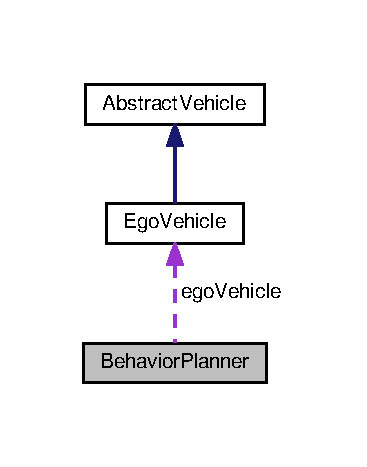
\includegraphics[width=176pt]{classBehaviorPlanner__coll__graph}
\end{center}
\end{figure}
\subsection*{Public Member Functions}
\begin{DoxyCompactItemize}
\item 
\hyperlink{classBehaviorPlanner_aef7c36cbc0cb70964a4e354037ed27a1}{Behavior\+Planner} (int initial\+Lane)
\item 
double \hyperlink{classBehaviorPlanner_aec0fc286b925dcc751af3c6caf3fdef9}{evaluate\+Situation} ()
\item 
double \hyperlink{classBehaviorPlanner_af0d483ed1b5e466fea8e94e3cfe62785}{evaluate\+Situation} (vector$<$ double $>$ ego\+Prediction, int prediction\+Horizon)
\item 
vector$<$ double $>$ \hyperlink{classBehaviorPlanner_a3a4c41036d3094e28f6b8f63b919e985}{predict\+Situation} (int prediction\+Horizon)
\item 
double \hyperlink{classBehaviorPlanner_ac786fd6c315da122b9269e2ef49b988d}{evaluate\+Lane} (vector$<$ double $>$ ego\+Prediction)
\item 
double \hyperlink{classBehaviorPlanner_aee55c3bbfbec8ab034069f15acfb40a6}{evaluate\+Safety\+Distance} (vector$<$ double $>$ ego\+Prediction, vector$<$ double $>$ object\+Prediction)
\item 
double \hyperlink{classBehaviorPlanner_acc2e5ddab8cd80c4fd789b08fcf60f5e}{evaluate\+Speed} (vector$<$ double $>$ ego\+Prediction, double ref\+Speed)
\item 
double \hyperlink{classBehaviorPlanner_aff22cd158b0d8a748e16eb4b9720d7a9}{evaluate\+Frenet\+\_\+d} (vector$<$ double $>$ ego\+Prediction)
\item 
int \hyperlink{classBehaviorPlanner_a833375362e34ebaeaff47005cd0bed6d}{evaluate\+Free\+Lane\+Bonus} (vector$<$ double $>$ ego\+Prediction, vector$<$ double $>$ object\+Prediction)
\item 
std\+::map$<$ double, \hyperlink{classSensorObject}{Sensor\+Object} $>$ \hyperlink{classBehaviorPlanner_ad45a4d61f54fde513d189734ff5b5899}{get\+Sensor\+Objects} ()
\item 
vector$<$ double $>$ \hyperlink{classBehaviorPlanner_a1e4a2c4125916f7533295982350da1d3}{get\+Maneuvr\+Data\+For\+Trajectory} (vector$<$ double $>$ proposed\+Path)
\item 
bool \hyperlink{classBehaviorPlanner_ace8509db32f1ee3ee4a178759b3fb32c}{stm\+\_\+lane\+\_\+change\+\_\+completed} ()
\end{DoxyCompactItemize}
\subsection*{Public Attributes}
\begin{DoxyCompactItemize}
\item 
std\+::map$<$ double, \hyperlink{classSensorObject}{Sensor\+Object} $>$ \hyperlink{classBehaviorPlanner_a0e7463db7467db3a4fe2e5eff7490d90}{sensor\+Objects}
\item 
\hyperlink{classEgoVehicle}{Ego\+Vehicle} \hyperlink{classBehaviorPlanner_a9dc8174e496e0ccf1d68bedec5b8fdb2}{ego\+Vehicle}
\end{DoxyCompactItemize}
\subsection*{Protected Member Functions}
\begin{DoxyCompactItemize}
\item 
bool \hyperlink{classBehaviorPlanner_ac3c4ecf02aa9deb5a0f955078090e3fd}{stm\+\_\+is\+Ready\+For\+Lane\+Change} ()
\item 
void \hyperlink{classBehaviorPlanner_aa4299becc244fb5f164921711da79fa5}{stm\+\_\+initiate\+Lane\+Change} (int target\+Lane)
\item 
vector$<$ vector$<$ vector$<$ double $>$ $>$ $>$ \hyperlink{classBehaviorPlanner_ae839573203455d697946581bbf58e662}{iterate\+Predictions} (vector$<$ double $>$ start, vector$<$ vector$<$ double $>$$>$ history, int prediction\+Horizon)
\end{DoxyCompactItemize}
\subsection*{Protected Attributes}
\begin{DoxyCompactItemize}
\item 
int \hyperlink{classBehaviorPlanner_a10df7163fdc6a3830a63cdf8a76b9359}{stm\+\_\+target\+\_\+lane}
\item 
bool \hyperlink{classBehaviorPlanner_aec3a75f12f6776616f4ecb275a975892}{stm\+\_\+is\+\_\+in\+\_\+lane\+\_\+change}
\item 
bool \hyperlink{classBehaviorPlanner_a78e0c9212796e8949f7f44bd34f47107}{stm\+\_\+ready\+\_\+for\+\_\+lane\+\_\+change}
\item 
double \hyperlink{classBehaviorPlanner_a13833c4fe873c4f5a85bd33fe8efc164}{evaluate\+Lane\+\_\+\+Weight} = 0.\+0
\item 
double \hyperlink{classBehaviorPlanner_a4793519effaf8f7c72794f28a3c92147}{evaluate\+Safety\+Distance\+\_\+\+Weight} = 10.\+0
\item 
double \hyperlink{classBehaviorPlanner_aeb4e5decdbd61adeb1e75da9d66ba34c}{evaluate\+Speed\+\_\+\+Weight} = 1.\+0
\item 
double \hyperlink{classBehaviorPlanner_a12260fe1c642173914fc2690337ac336}{evaluate\+Frenet\+\_\+d\+\_\+\+Weight} = 0.\+0
\end{DoxyCompactItemize}


\subsection{Constructor \& Destructor Documentation}
\index{Behavior\+Planner@{Behavior\+Planner}!Behavior\+Planner@{Behavior\+Planner}}
\index{Behavior\+Planner@{Behavior\+Planner}!Behavior\+Planner@{Behavior\+Planner}}
\subsubsection[{\texorpdfstring{Behavior\+Planner(int initial\+Lane)}{BehaviorPlanner(int initialLane)}}]{\setlength{\rightskip}{0pt plus 5cm}Behavior\+Planner\+::\+Behavior\+Planner (
\begin{DoxyParamCaption}
\item[{int}]{initial\+Lane}
\end{DoxyParamCaption}
)}\hypertarget{classBehaviorPlanner_aef7c36cbc0cb70964a4e354037ed27a1}{}\label{classBehaviorPlanner_aef7c36cbc0cb70964a4e354037ed27a1}


\subsection{Member Function Documentation}
\index{Behavior\+Planner@{Behavior\+Planner}!evaluate\+Free\+Lane\+Bonus@{evaluate\+Free\+Lane\+Bonus}}
\index{evaluate\+Free\+Lane\+Bonus@{evaluate\+Free\+Lane\+Bonus}!Behavior\+Planner@{Behavior\+Planner}}
\subsubsection[{\texorpdfstring{evaluate\+Free\+Lane\+Bonus(vector$<$ double $>$ ego\+Prediction, vector$<$ double $>$ object\+Prediction)}{evaluateFreeLaneBonus(vector< double > egoPrediction, vector< double > objectPrediction)}}]{\setlength{\rightskip}{0pt plus 5cm}int Behavior\+Planner\+::evaluate\+Free\+Lane\+Bonus (
\begin{DoxyParamCaption}
\item[{vector$<$ double $>$}]{ego\+Prediction, }
\item[{vector$<$ double $>$}]{object\+Prediction}
\end{DoxyParamCaption}
)}\hypertarget{classBehaviorPlanner_a833375362e34ebaeaff47005cd0bed6d}{}\label{classBehaviorPlanner_a833375362e34ebaeaff47005cd0bed6d}


Here is the call graph for this function\+:\nopagebreak
\begin{figure}[H]
\begin{center}
\leavevmode
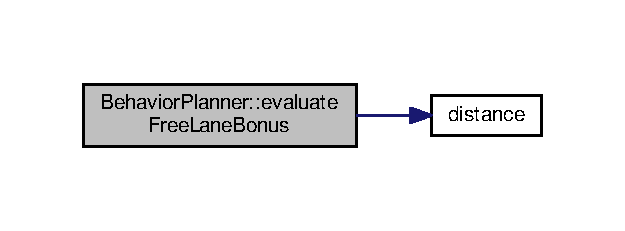
\includegraphics[width=300pt]{classBehaviorPlanner_a833375362e34ebaeaff47005cd0bed6d_cgraph}
\end{center}
\end{figure}


\index{Behavior\+Planner@{Behavior\+Planner}!evaluate\+Frenet\+\_\+d@{evaluate\+Frenet\+\_\+d}}
\index{evaluate\+Frenet\+\_\+d@{evaluate\+Frenet\+\_\+d}!Behavior\+Planner@{Behavior\+Planner}}
\subsubsection[{\texorpdfstring{evaluate\+Frenet\+\_\+d(vector$<$ double $>$ ego\+Prediction)}{evaluateFrenet_d(vector< double > egoPrediction)}}]{\setlength{\rightskip}{0pt plus 5cm}double Behavior\+Planner\+::evaluate\+Frenet\+\_\+d (
\begin{DoxyParamCaption}
\item[{vector$<$ double $>$}]{ego\+Prediction}
\end{DoxyParamCaption}
)}\hypertarget{classBehaviorPlanner_aff22cd158b0d8a748e16eb4b9720d7a9}{}\label{classBehaviorPlanner_aff22cd158b0d8a748e16eb4b9720d7a9}
\index{Behavior\+Planner@{Behavior\+Planner}!evaluate\+Lane@{evaluate\+Lane}}
\index{evaluate\+Lane@{evaluate\+Lane}!Behavior\+Planner@{Behavior\+Planner}}
\subsubsection[{\texorpdfstring{evaluate\+Lane(vector$<$ double $>$ ego\+Prediction)}{evaluateLane(vector< double > egoPrediction)}}]{\setlength{\rightskip}{0pt plus 5cm}double Behavior\+Planner\+::evaluate\+Lane (
\begin{DoxyParamCaption}
\item[{vector$<$ double $>$}]{ego\+Prediction}
\end{DoxyParamCaption}
)}\hypertarget{classBehaviorPlanner_ac786fd6c315da122b9269e2ef49b988d}{}\label{classBehaviorPlanner_ac786fd6c315da122b9269e2ef49b988d}
\index{Behavior\+Planner@{Behavior\+Planner}!evaluate\+Safety\+Distance@{evaluate\+Safety\+Distance}}
\index{evaluate\+Safety\+Distance@{evaluate\+Safety\+Distance}!Behavior\+Planner@{Behavior\+Planner}}
\subsubsection[{\texorpdfstring{evaluate\+Safety\+Distance(vector$<$ double $>$ ego\+Prediction, vector$<$ double $>$ object\+Prediction)}{evaluateSafetyDistance(vector< double > egoPrediction, vector< double > objectPrediction)}}]{\setlength{\rightskip}{0pt plus 5cm}double Behavior\+Planner\+::evaluate\+Safety\+Distance (
\begin{DoxyParamCaption}
\item[{vector$<$ double $>$}]{ego\+Prediction, }
\item[{vector$<$ double $>$}]{object\+Prediction}
\end{DoxyParamCaption}
)}\hypertarget{classBehaviorPlanner_aee55c3bbfbec8ab034069f15acfb40a6}{}\label{classBehaviorPlanner_aee55c3bbfbec8ab034069f15acfb40a6}


Here is the call graph for this function\+:\nopagebreak
\begin{figure}[H]
\begin{center}
\leavevmode
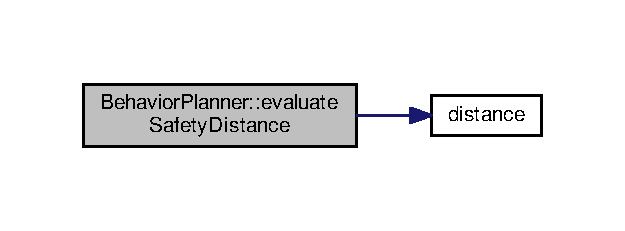
\includegraphics[width=300pt]{classBehaviorPlanner_aee55c3bbfbec8ab034069f15acfb40a6_cgraph}
\end{center}
\end{figure}


\index{Behavior\+Planner@{Behavior\+Planner}!evaluate\+Situation@{evaluate\+Situation}}
\index{evaluate\+Situation@{evaluate\+Situation}!Behavior\+Planner@{Behavior\+Planner}}
\subsubsection[{\texorpdfstring{evaluate\+Situation()}{evaluateSituation()}}]{\setlength{\rightskip}{0pt plus 5cm}double Behavior\+Planner\+::evaluate\+Situation (
\begin{DoxyParamCaption}
{}
\end{DoxyParamCaption}
)}\hypertarget{classBehaviorPlanner_aec0fc286b925dcc751af3c6caf3fdef9}{}\label{classBehaviorPlanner_aec0fc286b925dcc751af3c6caf3fdef9}
\index{Behavior\+Planner@{Behavior\+Planner}!evaluate\+Situation@{evaluate\+Situation}}
\index{evaluate\+Situation@{evaluate\+Situation}!Behavior\+Planner@{Behavior\+Planner}}
\subsubsection[{\texorpdfstring{evaluate\+Situation(vector$<$ double $>$ ego\+Prediction, int prediction\+Horizon)}{evaluateSituation(vector< double > egoPrediction, int predictionHorizon)}}]{\setlength{\rightskip}{0pt plus 5cm}double Behavior\+Planner\+::evaluate\+Situation (
\begin{DoxyParamCaption}
\item[{vector$<$ double $>$}]{ego\+Prediction, }
\item[{int}]{prediction\+Horizon}
\end{DoxyParamCaption}
)}\hypertarget{classBehaviorPlanner_af0d483ed1b5e466fea8e94e3cfe62785}{}\label{classBehaviorPlanner_af0d483ed1b5e466fea8e94e3cfe62785}
\index{Behavior\+Planner@{Behavior\+Planner}!evaluate\+Speed@{evaluate\+Speed}}
\index{evaluate\+Speed@{evaluate\+Speed}!Behavior\+Planner@{Behavior\+Planner}}
\subsubsection[{\texorpdfstring{evaluate\+Speed(vector$<$ double $>$ ego\+Prediction, double ref\+Speed)}{evaluateSpeed(vector< double > egoPrediction, double refSpeed)}}]{\setlength{\rightskip}{0pt plus 5cm}double Behavior\+Planner\+::evaluate\+Speed (
\begin{DoxyParamCaption}
\item[{vector$<$ double $>$}]{ego\+Prediction, }
\item[{double}]{ref\+Speed}
\end{DoxyParamCaption}
)}\hypertarget{classBehaviorPlanner_acc2e5ddab8cd80c4fd789b08fcf60f5e}{}\label{classBehaviorPlanner_acc2e5ddab8cd80c4fd789b08fcf60f5e}
\index{Behavior\+Planner@{Behavior\+Planner}!get\+Maneuvr\+Data\+For\+Trajectory@{get\+Maneuvr\+Data\+For\+Trajectory}}
\index{get\+Maneuvr\+Data\+For\+Trajectory@{get\+Maneuvr\+Data\+For\+Trajectory}!Behavior\+Planner@{Behavior\+Planner}}
\subsubsection[{\texorpdfstring{get\+Maneuvr\+Data\+For\+Trajectory(vector$<$ double $>$ proposed\+Path)}{getManeuvrDataForTrajectory(vector< double > proposedPath)}}]{\setlength{\rightskip}{0pt plus 5cm}vector$<$ double $>$ Behavior\+Planner\+::get\+Maneuvr\+Data\+For\+Trajectory (
\begin{DoxyParamCaption}
\item[{vector$<$ double $>$}]{proposed\+Path}
\end{DoxyParamCaption}
)}\hypertarget{classBehaviorPlanner_a1e4a2c4125916f7533295982350da1d3}{}\label{classBehaviorPlanner_a1e4a2c4125916f7533295982350da1d3}
\index{Behavior\+Planner@{Behavior\+Planner}!get\+Sensor\+Objects@{get\+Sensor\+Objects}}
\index{get\+Sensor\+Objects@{get\+Sensor\+Objects}!Behavior\+Planner@{Behavior\+Planner}}
\subsubsection[{\texorpdfstring{get\+Sensor\+Objects()}{getSensorObjects()}}]{\setlength{\rightskip}{0pt plus 5cm}std\+::map$<$double,{\bf Sensor\+Object}$>$ Behavior\+Planner\+::get\+Sensor\+Objects (
\begin{DoxyParamCaption}
{}
\end{DoxyParamCaption}
)\hspace{0.3cm}{\ttfamily [inline]}}\hypertarget{classBehaviorPlanner_ad45a4d61f54fde513d189734ff5b5899}{}\label{classBehaviorPlanner_ad45a4d61f54fde513d189734ff5b5899}
\index{Behavior\+Planner@{Behavior\+Planner}!iterate\+Predictions@{iterate\+Predictions}}
\index{iterate\+Predictions@{iterate\+Predictions}!Behavior\+Planner@{Behavior\+Planner}}
\subsubsection[{\texorpdfstring{iterate\+Predictions(vector$<$ double $>$ start, vector$<$ vector$<$ double $>$$>$ history, int prediction\+Horizon)}{iteratePredictions(vector< double > start, vector< vector< double >> history, int predictionHorizon)}}]{\setlength{\rightskip}{0pt plus 5cm}vector$<$ vector$<$ vector$<$ double $>$ $>$ $>$ Behavior\+Planner\+::iterate\+Predictions (
\begin{DoxyParamCaption}
\item[{vector$<$ double $>$}]{start, }
\item[{vector$<$ vector$<$ double $>$$>$}]{history, }
\item[{int}]{prediction\+Horizon}
\end{DoxyParamCaption}
)\hspace{0.3cm}{\ttfamily [protected]}}\hypertarget{classBehaviorPlanner_ae839573203455d697946581bbf58e662}{}\label{classBehaviorPlanner_ae839573203455d697946581bbf58e662}
\index{Behavior\+Planner@{Behavior\+Planner}!predict\+Situation@{predict\+Situation}}
\index{predict\+Situation@{predict\+Situation}!Behavior\+Planner@{Behavior\+Planner}}
\subsubsection[{\texorpdfstring{predict\+Situation(int prediction\+Horizon)}{predictSituation(int predictionHorizon)}}]{\setlength{\rightskip}{0pt plus 5cm}vector$<$ double $>$ Behavior\+Planner\+::predict\+Situation (
\begin{DoxyParamCaption}
\item[{int}]{prediction\+Horizon}
\end{DoxyParamCaption}
)}\hypertarget{classBehaviorPlanner_a3a4c41036d3094e28f6b8f63b919e985}{}\label{classBehaviorPlanner_a3a4c41036d3094e28f6b8f63b919e985}
\index{Behavior\+Planner@{Behavior\+Planner}!stm\+\_\+initiate\+Lane\+Change@{stm\+\_\+initiate\+Lane\+Change}}
\index{stm\+\_\+initiate\+Lane\+Change@{stm\+\_\+initiate\+Lane\+Change}!Behavior\+Planner@{Behavior\+Planner}}
\subsubsection[{\texorpdfstring{stm\+\_\+initiate\+Lane\+Change(int target\+Lane)}{stm_initiateLaneChange(int targetLane)}}]{\setlength{\rightskip}{0pt plus 5cm}void Behavior\+Planner\+::stm\+\_\+initiate\+Lane\+Change (
\begin{DoxyParamCaption}
\item[{int}]{target\+Lane}
\end{DoxyParamCaption}
)\hspace{0.3cm}{\ttfamily [protected]}}\hypertarget{classBehaviorPlanner_aa4299becc244fb5f164921711da79fa5}{}\label{classBehaviorPlanner_aa4299becc244fb5f164921711da79fa5}
\index{Behavior\+Planner@{Behavior\+Planner}!stm\+\_\+is\+Ready\+For\+Lane\+Change@{stm\+\_\+is\+Ready\+For\+Lane\+Change}}
\index{stm\+\_\+is\+Ready\+For\+Lane\+Change@{stm\+\_\+is\+Ready\+For\+Lane\+Change}!Behavior\+Planner@{Behavior\+Planner}}
\subsubsection[{\texorpdfstring{stm\+\_\+is\+Ready\+For\+Lane\+Change()}{stm_isReadyForLaneChange()}}]{\setlength{\rightskip}{0pt plus 5cm}bool Behavior\+Planner\+::stm\+\_\+is\+Ready\+For\+Lane\+Change (
\begin{DoxyParamCaption}
{}
\end{DoxyParamCaption}
)\hspace{0.3cm}{\ttfamily [protected]}}\hypertarget{classBehaviorPlanner_ac3c4ecf02aa9deb5a0f955078090e3fd}{}\label{classBehaviorPlanner_ac3c4ecf02aa9deb5a0f955078090e3fd}
\index{Behavior\+Planner@{Behavior\+Planner}!stm\+\_\+lane\+\_\+change\+\_\+completed@{stm\+\_\+lane\+\_\+change\+\_\+completed}}
\index{stm\+\_\+lane\+\_\+change\+\_\+completed@{stm\+\_\+lane\+\_\+change\+\_\+completed}!Behavior\+Planner@{Behavior\+Planner}}
\subsubsection[{\texorpdfstring{stm\+\_\+lane\+\_\+change\+\_\+completed()}{stm_lane_change_completed()}}]{\setlength{\rightskip}{0pt plus 5cm}bool Behavior\+Planner\+::stm\+\_\+lane\+\_\+change\+\_\+completed (
\begin{DoxyParamCaption}
{}
\end{DoxyParamCaption}
)}\hypertarget{classBehaviorPlanner_ace8509db32f1ee3ee4a178759b3fb32c}{}\label{classBehaviorPlanner_ace8509db32f1ee3ee4a178759b3fb32c}


\subsection{Member Data Documentation}
\index{Behavior\+Planner@{Behavior\+Planner}!ego\+Vehicle@{ego\+Vehicle}}
\index{ego\+Vehicle@{ego\+Vehicle}!Behavior\+Planner@{Behavior\+Planner}}
\subsubsection[{\texorpdfstring{ego\+Vehicle}{egoVehicle}}]{\setlength{\rightskip}{0pt plus 5cm}{\bf Ego\+Vehicle} Behavior\+Planner\+::ego\+Vehicle}\hypertarget{classBehaviorPlanner_a9dc8174e496e0ccf1d68bedec5b8fdb2}{}\label{classBehaviorPlanner_a9dc8174e496e0ccf1d68bedec5b8fdb2}
\index{Behavior\+Planner@{Behavior\+Planner}!evaluate\+Frenet\+\_\+d\+\_\+\+Weight@{evaluate\+Frenet\+\_\+d\+\_\+\+Weight}}
\index{evaluate\+Frenet\+\_\+d\+\_\+\+Weight@{evaluate\+Frenet\+\_\+d\+\_\+\+Weight}!Behavior\+Planner@{Behavior\+Planner}}
\subsubsection[{\texorpdfstring{evaluate\+Frenet\+\_\+d\+\_\+\+Weight}{evaluateFrenet_d_Weight}}]{\setlength{\rightskip}{0pt plus 5cm}double Behavior\+Planner\+::evaluate\+Frenet\+\_\+d\+\_\+\+Weight = 0.\+0\hspace{0.3cm}{\ttfamily [protected]}}\hypertarget{classBehaviorPlanner_a12260fe1c642173914fc2690337ac336}{}\label{classBehaviorPlanner_a12260fe1c642173914fc2690337ac336}
\index{Behavior\+Planner@{Behavior\+Planner}!evaluate\+Lane\+\_\+\+Weight@{evaluate\+Lane\+\_\+\+Weight}}
\index{evaluate\+Lane\+\_\+\+Weight@{evaluate\+Lane\+\_\+\+Weight}!Behavior\+Planner@{Behavior\+Planner}}
\subsubsection[{\texorpdfstring{evaluate\+Lane\+\_\+\+Weight}{evaluateLane_Weight}}]{\setlength{\rightskip}{0pt plus 5cm}double Behavior\+Planner\+::evaluate\+Lane\+\_\+\+Weight = 0.\+0\hspace{0.3cm}{\ttfamily [protected]}}\hypertarget{classBehaviorPlanner_a13833c4fe873c4f5a85bd33fe8efc164}{}\label{classBehaviorPlanner_a13833c4fe873c4f5a85bd33fe8efc164}
\index{Behavior\+Planner@{Behavior\+Planner}!evaluate\+Safety\+Distance\+\_\+\+Weight@{evaluate\+Safety\+Distance\+\_\+\+Weight}}
\index{evaluate\+Safety\+Distance\+\_\+\+Weight@{evaluate\+Safety\+Distance\+\_\+\+Weight}!Behavior\+Planner@{Behavior\+Planner}}
\subsubsection[{\texorpdfstring{evaluate\+Safety\+Distance\+\_\+\+Weight}{evaluateSafetyDistance_Weight}}]{\setlength{\rightskip}{0pt plus 5cm}double Behavior\+Planner\+::evaluate\+Safety\+Distance\+\_\+\+Weight = 10.\+0\hspace{0.3cm}{\ttfamily [protected]}}\hypertarget{classBehaviorPlanner_a4793519effaf8f7c72794f28a3c92147}{}\label{classBehaviorPlanner_a4793519effaf8f7c72794f28a3c92147}
\index{Behavior\+Planner@{Behavior\+Planner}!evaluate\+Speed\+\_\+\+Weight@{evaluate\+Speed\+\_\+\+Weight}}
\index{evaluate\+Speed\+\_\+\+Weight@{evaluate\+Speed\+\_\+\+Weight}!Behavior\+Planner@{Behavior\+Planner}}
\subsubsection[{\texorpdfstring{evaluate\+Speed\+\_\+\+Weight}{evaluateSpeed_Weight}}]{\setlength{\rightskip}{0pt plus 5cm}double Behavior\+Planner\+::evaluate\+Speed\+\_\+\+Weight = 1.\+0\hspace{0.3cm}{\ttfamily [protected]}}\hypertarget{classBehaviorPlanner_aeb4e5decdbd61adeb1e75da9d66ba34c}{}\label{classBehaviorPlanner_aeb4e5decdbd61adeb1e75da9d66ba34c}
\index{Behavior\+Planner@{Behavior\+Planner}!sensor\+Objects@{sensor\+Objects}}
\index{sensor\+Objects@{sensor\+Objects}!Behavior\+Planner@{Behavior\+Planner}}
\subsubsection[{\texorpdfstring{sensor\+Objects}{sensorObjects}}]{\setlength{\rightskip}{0pt plus 5cm}std\+::map$<$double,{\bf Sensor\+Object}$>$ Behavior\+Planner\+::sensor\+Objects}\hypertarget{classBehaviorPlanner_a0e7463db7467db3a4fe2e5eff7490d90}{}\label{classBehaviorPlanner_a0e7463db7467db3a4fe2e5eff7490d90}
\index{Behavior\+Planner@{Behavior\+Planner}!stm\+\_\+is\+\_\+in\+\_\+lane\+\_\+change@{stm\+\_\+is\+\_\+in\+\_\+lane\+\_\+change}}
\index{stm\+\_\+is\+\_\+in\+\_\+lane\+\_\+change@{stm\+\_\+is\+\_\+in\+\_\+lane\+\_\+change}!Behavior\+Planner@{Behavior\+Planner}}
\subsubsection[{\texorpdfstring{stm\+\_\+is\+\_\+in\+\_\+lane\+\_\+change}{stm_is_in_lane_change}}]{\setlength{\rightskip}{0pt plus 5cm}bool Behavior\+Planner\+::stm\+\_\+is\+\_\+in\+\_\+lane\+\_\+change\hspace{0.3cm}{\ttfamily [protected]}}\hypertarget{classBehaviorPlanner_aec3a75f12f6776616f4ecb275a975892}{}\label{classBehaviorPlanner_aec3a75f12f6776616f4ecb275a975892}
\index{Behavior\+Planner@{Behavior\+Planner}!stm\+\_\+ready\+\_\+for\+\_\+lane\+\_\+change@{stm\+\_\+ready\+\_\+for\+\_\+lane\+\_\+change}}
\index{stm\+\_\+ready\+\_\+for\+\_\+lane\+\_\+change@{stm\+\_\+ready\+\_\+for\+\_\+lane\+\_\+change}!Behavior\+Planner@{Behavior\+Planner}}
\subsubsection[{\texorpdfstring{stm\+\_\+ready\+\_\+for\+\_\+lane\+\_\+change}{stm_ready_for_lane_change}}]{\setlength{\rightskip}{0pt plus 5cm}bool Behavior\+Planner\+::stm\+\_\+ready\+\_\+for\+\_\+lane\+\_\+change\hspace{0.3cm}{\ttfamily [protected]}}\hypertarget{classBehaviorPlanner_a78e0c9212796e8949f7f44bd34f47107}{}\label{classBehaviorPlanner_a78e0c9212796e8949f7f44bd34f47107}
\index{Behavior\+Planner@{Behavior\+Planner}!stm\+\_\+target\+\_\+lane@{stm\+\_\+target\+\_\+lane}}
\index{stm\+\_\+target\+\_\+lane@{stm\+\_\+target\+\_\+lane}!Behavior\+Planner@{Behavior\+Planner}}
\subsubsection[{\texorpdfstring{stm\+\_\+target\+\_\+lane}{stm_target_lane}}]{\setlength{\rightskip}{0pt plus 5cm}int Behavior\+Planner\+::stm\+\_\+target\+\_\+lane\hspace{0.3cm}{\ttfamily [protected]}}\hypertarget{classBehaviorPlanner_a10df7163fdc6a3830a63cdf8a76b9359}{}\label{classBehaviorPlanner_a10df7163fdc6a3830a63cdf8a76b9359}


The documentation for this class was generated from the following files\+:\begin{DoxyCompactItemize}
\item 
src/\hyperlink{BehaviorPlanner_8h}{Behavior\+Planner.\+h}\item 
src/\hyperlink{BehaviorPlanner_8cpp}{Behavior\+Planner.\+cpp}\end{DoxyCompactItemize}

\hypertarget{classEgoVehicle}{}\section{Ego\+Vehicle Class Reference}
\label{classEgoVehicle}\index{Ego\+Vehicle@{Ego\+Vehicle}}


{\ttfamily \#include $<$Ego\+Vehicle.\+h$>$}



Inheritance diagram for Ego\+Vehicle\+:\nopagebreak
\begin{figure}[H]
\begin{center}
\leavevmode
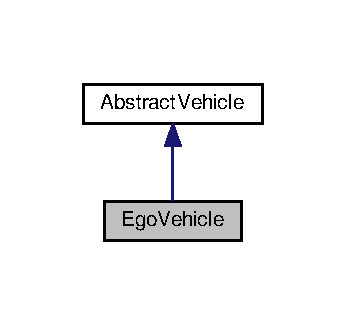
\includegraphics[width=166pt]{classEgoVehicle__inherit__graph}
\end{center}
\end{figure}


Collaboration diagram for Ego\+Vehicle\+:\nopagebreak
\begin{figure}[H]
\begin{center}
\leavevmode
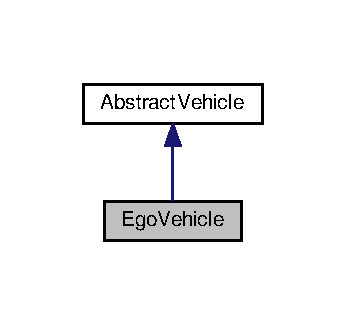
\includegraphics[width=166pt]{classEgoVehicle__coll__graph}
\end{center}
\end{figure}
\subsection*{Public Member Functions}
\begin{DoxyCompactItemize}
\item 
\hyperlink{classEgoVehicle_a2fdc6347881fa4a7a629642f0bbacd82}{Ego\+Vehicle} ()
\item 
double \hyperlink{classEgoVehicle_a8062f2bbb14f1bd787921cd83d4e5475}{get\+Speed} ()
\item 
double \hyperlink{classEgoVehicle_a692add014c4846c554c4d08e170c140a}{get\+Speed\+\_\+x} ()
\item 
double \hyperlink{classEgoVehicle_a88d4bc1d06c685f060d8e628452173fb}{get\+Speed\+\_\+y} ()
\item 
string \hyperlink{classEgoVehicle_a68e3c46400e34d4f805fcc392ecd5563}{display} ()
\item 
void \hyperlink{classEgoVehicle_a5ba202f45ceff0e164f55a7e1535a178}{set\+Ref\+Speed} (double \hyperlink{classEgoVehicle_a80a9ae1a27a7368cd10f22ac08edcbd3}{ref\+Speed}=10)
\item 
double \hyperlink{classEgoVehicle_a487b97b4bb6f969dc032e1387fc3f26f}{get\+Ref\+Speed} ()
\item 
void \hyperlink{classEgoVehicle_ae189735224d6a6bb46f6170321c128dc}{update} (\hyperlink{main_8cpp_ab701e3ac61a85b337ec5c1abaad6742d}{json} j)
\item 
vector$<$ double $>$ \hyperlink{classEgoVehicle_a6ee0af573a8c20a127f954c5237121c5}{get\+Previous\+\_\+path\+\_\+x} ()
\item 
vector$<$ double $>$ \hyperlink{classEgoVehicle_ad87d6b79a64ddae062f3a70575263091}{get\+Previous\+\_\+path\+\_\+y} ()
\item 
double \hyperlink{classEgoVehicle_a2f819cd37b15262c2751aaec5f78e4df}{get\+Yaw\+Rad} ()
\item 
double \hyperlink{classEgoVehicle_aa75a2d9f4457d5bf249acc0e4672d327}{get\+Yaw\+Deg} ()
\item 
double \hyperlink{classEgoVehicle_a4bc481d854046754ad80e5106e82c685}{get\+End\+\_\+\+Path\+\_\+s} ()
\item 
double \hyperlink{classEgoVehicle_ae6341fe7bd256601b267cd1a3f122ac0}{get\+End\+\_\+\+Path\+\_\+d} ()
\item 
vector$<$ double $>$ \hyperlink{classEgoVehicle_af44e6b8bb8af7410ea404b8939507c93}{get\+Prediction} (int second)
\item 
void \hyperlink{classEgoVehicle_ae0b5afee444e02d3211d1bc0c6524bbe}{calculate\+Predictions} (int prediction\+Horizon)
\end{DoxyCompactItemize}
\subsection*{Protected Attributes}
\begin{DoxyCompactItemize}
\item 
double \hyperlink{classEgoVehicle_a80a9ae1a27a7368cd10f22ac08edcbd3}{ref\+Speed}
\item 
double \hyperlink{classEgoVehicle_ae99585d114a39d671d04c19da303e473}{yaw}
\item 
vector$<$ double $>$ \hyperlink{classEgoVehicle_ae32d68e714c98e6e81f15bc9959ffb9e}{previous\+\_\+path\+\_\+x}
\item 
vector$<$ double $>$ \hyperlink{classEgoVehicle_aaf1ac96664e7d8e608c710329eed2a3d}{previous\+\_\+path\+\_\+y}
\item 
double \hyperlink{classEgoVehicle_ae60f078c638261d10fac67b96681cd4a}{end\+\_\+path\+\_\+s}
\item 
double \hyperlink{classEgoVehicle_ab12c04925764e5963d51d5b15b491f4e}{end\+\_\+path\+\_\+d}
\item 
double \hyperlink{classEgoVehicle_af0238faf0f998a051b04417bff609315}{speed\+\_\+from\+\_\+sim}
\end{DoxyCompactItemize}


\subsection{Constructor \& Destructor Documentation}
\index{Ego\+Vehicle@{Ego\+Vehicle}!Ego\+Vehicle@{Ego\+Vehicle}}
\index{Ego\+Vehicle@{Ego\+Vehicle}!Ego\+Vehicle@{Ego\+Vehicle}}
\subsubsection[{\texorpdfstring{Ego\+Vehicle()}{EgoVehicle()}}]{\setlength{\rightskip}{0pt plus 5cm}Ego\+Vehicle\+::\+Ego\+Vehicle (
\begin{DoxyParamCaption}
{}
\end{DoxyParamCaption}
)}\hypertarget{classEgoVehicle_a2fdc6347881fa4a7a629642f0bbacd82}{}\label{classEgoVehicle_a2fdc6347881fa4a7a629642f0bbacd82}


\subsection{Member Function Documentation}
\index{Ego\+Vehicle@{Ego\+Vehicle}!calculate\+Predictions@{calculate\+Predictions}}
\index{calculate\+Predictions@{calculate\+Predictions}!Ego\+Vehicle@{Ego\+Vehicle}}
\subsubsection[{\texorpdfstring{calculate\+Predictions(int prediction\+Horizon)}{calculatePredictions(int predictionHorizon)}}]{\setlength{\rightskip}{0pt plus 5cm}void Ego\+Vehicle\+::calculate\+Predictions (
\begin{DoxyParamCaption}
\item[{int}]{prediction\+Horizon}
\end{DoxyParamCaption}
)\hspace{0.3cm}{\ttfamily [virtual]}}\hypertarget{classEgoVehicle_ae0b5afee444e02d3211d1bc0c6524bbe}{}\label{classEgoVehicle_ae0b5afee444e02d3211d1bc0c6524bbe}


Implements \hyperlink{classAbstractVehicle_a631115b44756050ccf2a7fe975787035}{Abstract\+Vehicle}.

\index{Ego\+Vehicle@{Ego\+Vehicle}!display@{display}}
\index{display@{display}!Ego\+Vehicle@{Ego\+Vehicle}}
\subsubsection[{\texorpdfstring{display()}{display()}}]{\setlength{\rightskip}{0pt plus 5cm}string Ego\+Vehicle\+::display (
\begin{DoxyParamCaption}
{}
\end{DoxyParamCaption}
)\hspace{0.3cm}{\ttfamily [virtual]}}\hypertarget{classEgoVehicle_a68e3c46400e34d4f805fcc392ecd5563}{}\label{classEgoVehicle_a68e3c46400e34d4f805fcc392ecd5563}


Implements \hyperlink{classAbstractVehicle_ada311ec475179ba776966f7e3ddcb91a}{Abstract\+Vehicle}.



Here is the call graph for this function\+:\nopagebreak
\begin{figure}[H]
\begin{center}
\leavevmode
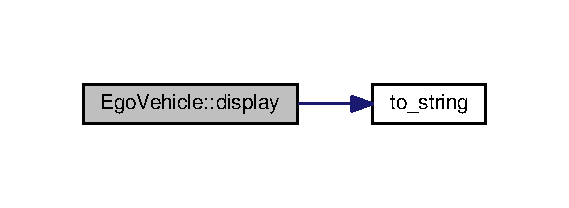
\includegraphics[width=273pt]{classEgoVehicle_a68e3c46400e34d4f805fcc392ecd5563_cgraph}
\end{center}
\end{figure}


\index{Ego\+Vehicle@{Ego\+Vehicle}!get\+End\+\_\+\+Path\+\_\+d@{get\+End\+\_\+\+Path\+\_\+d}}
\index{get\+End\+\_\+\+Path\+\_\+d@{get\+End\+\_\+\+Path\+\_\+d}!Ego\+Vehicle@{Ego\+Vehicle}}
\subsubsection[{\texorpdfstring{get\+End\+\_\+\+Path\+\_\+d()}{getEnd_Path_d()}}]{\setlength{\rightskip}{0pt plus 5cm}double Ego\+Vehicle\+::get\+End\+\_\+\+Path\+\_\+d (
\begin{DoxyParamCaption}
{}
\end{DoxyParamCaption}
)\hspace{0.3cm}{\ttfamily [inline]}}\hypertarget{classEgoVehicle_ae6341fe7bd256601b267cd1a3f122ac0}{}\label{classEgoVehicle_ae6341fe7bd256601b267cd1a3f122ac0}
\index{Ego\+Vehicle@{Ego\+Vehicle}!get\+End\+\_\+\+Path\+\_\+s@{get\+End\+\_\+\+Path\+\_\+s}}
\index{get\+End\+\_\+\+Path\+\_\+s@{get\+End\+\_\+\+Path\+\_\+s}!Ego\+Vehicle@{Ego\+Vehicle}}
\subsubsection[{\texorpdfstring{get\+End\+\_\+\+Path\+\_\+s()}{getEnd_Path_s()}}]{\setlength{\rightskip}{0pt plus 5cm}double Ego\+Vehicle\+::get\+End\+\_\+\+Path\+\_\+s (
\begin{DoxyParamCaption}
{}
\end{DoxyParamCaption}
)\hspace{0.3cm}{\ttfamily [inline]}}\hypertarget{classEgoVehicle_a4bc481d854046754ad80e5106e82c685}{}\label{classEgoVehicle_a4bc481d854046754ad80e5106e82c685}
\index{Ego\+Vehicle@{Ego\+Vehicle}!get\+Prediction@{get\+Prediction}}
\index{get\+Prediction@{get\+Prediction}!Ego\+Vehicle@{Ego\+Vehicle}}
\subsubsection[{\texorpdfstring{get\+Prediction(int second)}{getPrediction(int second)}}]{\setlength{\rightskip}{0pt plus 5cm}vector$<$ double $>$ Ego\+Vehicle\+::get\+Prediction (
\begin{DoxyParamCaption}
\item[{int}]{second}
\end{DoxyParamCaption}
)\hspace{0.3cm}{\ttfamily [virtual]}}\hypertarget{classEgoVehicle_af44e6b8bb8af7410ea404b8939507c93}{}\label{classEgoVehicle_af44e6b8bb8af7410ea404b8939507c93}


Implements \hyperlink{classAbstractVehicle_a3c84d6970c9461bfafd76cf48d6bece0}{Abstract\+Vehicle}.

\index{Ego\+Vehicle@{Ego\+Vehicle}!get\+Previous\+\_\+path\+\_\+x@{get\+Previous\+\_\+path\+\_\+x}}
\index{get\+Previous\+\_\+path\+\_\+x@{get\+Previous\+\_\+path\+\_\+x}!Ego\+Vehicle@{Ego\+Vehicle}}
\subsubsection[{\texorpdfstring{get\+Previous\+\_\+path\+\_\+x()}{getPrevious_path_x()}}]{\setlength{\rightskip}{0pt plus 5cm}vector$<$double$>$ Ego\+Vehicle\+::get\+Previous\+\_\+path\+\_\+x (
\begin{DoxyParamCaption}
{}
\end{DoxyParamCaption}
)\hspace{0.3cm}{\ttfamily [inline]}}\hypertarget{classEgoVehicle_a6ee0af573a8c20a127f954c5237121c5}{}\label{classEgoVehicle_a6ee0af573a8c20a127f954c5237121c5}
\index{Ego\+Vehicle@{Ego\+Vehicle}!get\+Previous\+\_\+path\+\_\+y@{get\+Previous\+\_\+path\+\_\+y}}
\index{get\+Previous\+\_\+path\+\_\+y@{get\+Previous\+\_\+path\+\_\+y}!Ego\+Vehicle@{Ego\+Vehicle}}
\subsubsection[{\texorpdfstring{get\+Previous\+\_\+path\+\_\+y()}{getPrevious_path_y()}}]{\setlength{\rightskip}{0pt plus 5cm}vector$<$double$>$ Ego\+Vehicle\+::get\+Previous\+\_\+path\+\_\+y (
\begin{DoxyParamCaption}
{}
\end{DoxyParamCaption}
)\hspace{0.3cm}{\ttfamily [inline]}}\hypertarget{classEgoVehicle_ad87d6b79a64ddae062f3a70575263091}{}\label{classEgoVehicle_ad87d6b79a64ddae062f3a70575263091}
\index{Ego\+Vehicle@{Ego\+Vehicle}!get\+Ref\+Speed@{get\+Ref\+Speed}}
\index{get\+Ref\+Speed@{get\+Ref\+Speed}!Ego\+Vehicle@{Ego\+Vehicle}}
\subsubsection[{\texorpdfstring{get\+Ref\+Speed()}{getRefSpeed()}}]{\setlength{\rightskip}{0pt plus 5cm}double Ego\+Vehicle\+::get\+Ref\+Speed (
\begin{DoxyParamCaption}
{}
\end{DoxyParamCaption}
)}\hypertarget{classEgoVehicle_a487b97b4bb6f969dc032e1387fc3f26f}{}\label{classEgoVehicle_a487b97b4bb6f969dc032e1387fc3f26f}
\index{Ego\+Vehicle@{Ego\+Vehicle}!get\+Speed@{get\+Speed}}
\index{get\+Speed@{get\+Speed}!Ego\+Vehicle@{Ego\+Vehicle}}
\subsubsection[{\texorpdfstring{get\+Speed()}{getSpeed()}}]{\setlength{\rightskip}{0pt plus 5cm}double Ego\+Vehicle\+::get\+Speed (
\begin{DoxyParamCaption}
{}
\end{DoxyParamCaption}
)\hspace{0.3cm}{\ttfamily [virtual]}}\hypertarget{classEgoVehicle_a8062f2bbb14f1bd787921cd83d4e5475}{}\label{classEgoVehicle_a8062f2bbb14f1bd787921cd83d4e5475}


Implements \hyperlink{classAbstractVehicle_a17c193d56e1da24a1008ae52859d31c7}{Abstract\+Vehicle}.

\index{Ego\+Vehicle@{Ego\+Vehicle}!get\+Speed\+\_\+x@{get\+Speed\+\_\+x}}
\index{get\+Speed\+\_\+x@{get\+Speed\+\_\+x}!Ego\+Vehicle@{Ego\+Vehicle}}
\subsubsection[{\texorpdfstring{get\+Speed\+\_\+x()}{getSpeed_x()}}]{\setlength{\rightskip}{0pt plus 5cm}double Ego\+Vehicle\+::get\+Speed\+\_\+x (
\begin{DoxyParamCaption}
{}
\end{DoxyParamCaption}
)\hspace{0.3cm}{\ttfamily [virtual]}}\hypertarget{classEgoVehicle_a692add014c4846c554c4d08e170c140a}{}\label{classEgoVehicle_a692add014c4846c554c4d08e170c140a}


Implements \hyperlink{classAbstractVehicle_abe9a9f5e2290fdf4207ac0206b9e97a3}{Abstract\+Vehicle}.

\index{Ego\+Vehicle@{Ego\+Vehicle}!get\+Speed\+\_\+y@{get\+Speed\+\_\+y}}
\index{get\+Speed\+\_\+y@{get\+Speed\+\_\+y}!Ego\+Vehicle@{Ego\+Vehicle}}
\subsubsection[{\texorpdfstring{get\+Speed\+\_\+y()}{getSpeed_y()}}]{\setlength{\rightskip}{0pt plus 5cm}double Ego\+Vehicle\+::get\+Speed\+\_\+y (
\begin{DoxyParamCaption}
{}
\end{DoxyParamCaption}
)\hspace{0.3cm}{\ttfamily [virtual]}}\hypertarget{classEgoVehicle_a88d4bc1d06c685f060d8e628452173fb}{}\label{classEgoVehicle_a88d4bc1d06c685f060d8e628452173fb}


Implements \hyperlink{classAbstractVehicle_a90e6e4299070bace1acfd8d79bf78c95}{Abstract\+Vehicle}.

\index{Ego\+Vehicle@{Ego\+Vehicle}!get\+Yaw\+Deg@{get\+Yaw\+Deg}}
\index{get\+Yaw\+Deg@{get\+Yaw\+Deg}!Ego\+Vehicle@{Ego\+Vehicle}}
\subsubsection[{\texorpdfstring{get\+Yaw\+Deg()}{getYawDeg()}}]{\setlength{\rightskip}{0pt plus 5cm}double Ego\+Vehicle\+::get\+Yaw\+Deg (
\begin{DoxyParamCaption}
{}
\end{DoxyParamCaption}
)\hspace{0.3cm}{\ttfamily [inline]}}\hypertarget{classEgoVehicle_aa75a2d9f4457d5bf249acc0e4672d327}{}\label{classEgoVehicle_aa75a2d9f4457d5bf249acc0e4672d327}
\index{Ego\+Vehicle@{Ego\+Vehicle}!get\+Yaw\+Rad@{get\+Yaw\+Rad}}
\index{get\+Yaw\+Rad@{get\+Yaw\+Rad}!Ego\+Vehicle@{Ego\+Vehicle}}
\subsubsection[{\texorpdfstring{get\+Yaw\+Rad()}{getYawRad()}}]{\setlength{\rightskip}{0pt plus 5cm}double Ego\+Vehicle\+::get\+Yaw\+Rad (
\begin{DoxyParamCaption}
{}
\end{DoxyParamCaption}
)\hspace{0.3cm}{\ttfamily [inline]}}\hypertarget{classEgoVehicle_a2f819cd37b15262c2751aaec5f78e4df}{}\label{classEgoVehicle_a2f819cd37b15262c2751aaec5f78e4df}
\index{Ego\+Vehicle@{Ego\+Vehicle}!set\+Ref\+Speed@{set\+Ref\+Speed}}
\index{set\+Ref\+Speed@{set\+Ref\+Speed}!Ego\+Vehicle@{Ego\+Vehicle}}
\subsubsection[{\texorpdfstring{set\+Ref\+Speed(double ref\+Speed=10)}{setRefSpeed(double refSpeed=10)}}]{\setlength{\rightskip}{0pt plus 5cm}void Ego\+Vehicle\+::set\+Ref\+Speed (
\begin{DoxyParamCaption}
\item[{double}]{ref\+Speed = {\ttfamily 10}}
\end{DoxyParamCaption}
)}\hypertarget{classEgoVehicle_a5ba202f45ceff0e164f55a7e1535a178}{}\label{classEgoVehicle_a5ba202f45ceff0e164f55a7e1535a178}
\index{Ego\+Vehicle@{Ego\+Vehicle}!update@{update}}
\index{update@{update}!Ego\+Vehicle@{Ego\+Vehicle}}
\subsubsection[{\texorpdfstring{update(json j)}{update(json j)}}]{\setlength{\rightskip}{0pt plus 5cm}void Ego\+Vehicle\+::update (
\begin{DoxyParamCaption}
\item[{{\bf json}}]{j}
\end{DoxyParamCaption}
)\hspace{0.3cm}{\ttfamily [virtual]}}\hypertarget{classEgoVehicle_ae189735224d6a6bb46f6170321c128dc}{}\label{classEgoVehicle_ae189735224d6a6bb46f6170321c128dc}


Implements \hyperlink{classAbstractVehicle_a004b43b4a4d02ca6122ed8862c672de3}{Abstract\+Vehicle}.



\subsection{Member Data Documentation}
\index{Ego\+Vehicle@{Ego\+Vehicle}!end\+\_\+path\+\_\+d@{end\+\_\+path\+\_\+d}}
\index{end\+\_\+path\+\_\+d@{end\+\_\+path\+\_\+d}!Ego\+Vehicle@{Ego\+Vehicle}}
\subsubsection[{\texorpdfstring{end\+\_\+path\+\_\+d}{end_path_d}}]{\setlength{\rightskip}{0pt plus 5cm}double Ego\+Vehicle\+::end\+\_\+path\+\_\+d\hspace{0.3cm}{\ttfamily [protected]}}\hypertarget{classEgoVehicle_ab12c04925764e5963d51d5b15b491f4e}{}\label{classEgoVehicle_ab12c04925764e5963d51d5b15b491f4e}
\index{Ego\+Vehicle@{Ego\+Vehicle}!end\+\_\+path\+\_\+s@{end\+\_\+path\+\_\+s}}
\index{end\+\_\+path\+\_\+s@{end\+\_\+path\+\_\+s}!Ego\+Vehicle@{Ego\+Vehicle}}
\subsubsection[{\texorpdfstring{end\+\_\+path\+\_\+s}{end_path_s}}]{\setlength{\rightskip}{0pt plus 5cm}double Ego\+Vehicle\+::end\+\_\+path\+\_\+s\hspace{0.3cm}{\ttfamily [protected]}}\hypertarget{classEgoVehicle_ae60f078c638261d10fac67b96681cd4a}{}\label{classEgoVehicle_ae60f078c638261d10fac67b96681cd4a}
\index{Ego\+Vehicle@{Ego\+Vehicle}!previous\+\_\+path\+\_\+x@{previous\+\_\+path\+\_\+x}}
\index{previous\+\_\+path\+\_\+x@{previous\+\_\+path\+\_\+x}!Ego\+Vehicle@{Ego\+Vehicle}}
\subsubsection[{\texorpdfstring{previous\+\_\+path\+\_\+x}{previous_path_x}}]{\setlength{\rightskip}{0pt plus 5cm}vector$<$double$>$ Ego\+Vehicle\+::previous\+\_\+path\+\_\+x\hspace{0.3cm}{\ttfamily [protected]}}\hypertarget{classEgoVehicle_ae32d68e714c98e6e81f15bc9959ffb9e}{}\label{classEgoVehicle_ae32d68e714c98e6e81f15bc9959ffb9e}
\index{Ego\+Vehicle@{Ego\+Vehicle}!previous\+\_\+path\+\_\+y@{previous\+\_\+path\+\_\+y}}
\index{previous\+\_\+path\+\_\+y@{previous\+\_\+path\+\_\+y}!Ego\+Vehicle@{Ego\+Vehicle}}
\subsubsection[{\texorpdfstring{previous\+\_\+path\+\_\+y}{previous_path_y}}]{\setlength{\rightskip}{0pt plus 5cm}vector$<$double$>$ Ego\+Vehicle\+::previous\+\_\+path\+\_\+y\hspace{0.3cm}{\ttfamily [protected]}}\hypertarget{classEgoVehicle_aaf1ac96664e7d8e608c710329eed2a3d}{}\label{classEgoVehicle_aaf1ac96664e7d8e608c710329eed2a3d}
\index{Ego\+Vehicle@{Ego\+Vehicle}!ref\+Speed@{ref\+Speed}}
\index{ref\+Speed@{ref\+Speed}!Ego\+Vehicle@{Ego\+Vehicle}}
\subsubsection[{\texorpdfstring{ref\+Speed}{refSpeed}}]{\setlength{\rightskip}{0pt plus 5cm}double Ego\+Vehicle\+::ref\+Speed\hspace{0.3cm}{\ttfamily [protected]}}\hypertarget{classEgoVehicle_a80a9ae1a27a7368cd10f22ac08edcbd3}{}\label{classEgoVehicle_a80a9ae1a27a7368cd10f22ac08edcbd3}
\index{Ego\+Vehicle@{Ego\+Vehicle}!speed\+\_\+from\+\_\+sim@{speed\+\_\+from\+\_\+sim}}
\index{speed\+\_\+from\+\_\+sim@{speed\+\_\+from\+\_\+sim}!Ego\+Vehicle@{Ego\+Vehicle}}
\subsubsection[{\texorpdfstring{speed\+\_\+from\+\_\+sim}{speed_from_sim}}]{\setlength{\rightskip}{0pt plus 5cm}double Ego\+Vehicle\+::speed\+\_\+from\+\_\+sim\hspace{0.3cm}{\ttfamily [protected]}}\hypertarget{classEgoVehicle_af0238faf0f998a051b04417bff609315}{}\label{classEgoVehicle_af0238faf0f998a051b04417bff609315}
\index{Ego\+Vehicle@{Ego\+Vehicle}!yaw@{yaw}}
\index{yaw@{yaw}!Ego\+Vehicle@{Ego\+Vehicle}}
\subsubsection[{\texorpdfstring{yaw}{yaw}}]{\setlength{\rightskip}{0pt plus 5cm}double Ego\+Vehicle\+::yaw\hspace{0.3cm}{\ttfamily [protected]}}\hypertarget{classEgoVehicle_ae99585d114a39d671d04c19da303e473}{}\label{classEgoVehicle_ae99585d114a39d671d04c19da303e473}


The documentation for this class was generated from the following files\+:\begin{DoxyCompactItemize}
\item 
src/\hyperlink{EgoVehicle_8h}{Ego\+Vehicle.\+h}\item 
src/\hyperlink{EgoVehicle_8cpp}{Ego\+Vehicle.\+cpp}\end{DoxyCompactItemize}

\hypertarget{classSensorObject}{}\section{Sensor\+Object Class Reference}
\label{classSensorObject}\index{Sensor\+Object@{Sensor\+Object}}


{\ttfamily \#include $<$Sensor\+Object.\+h$>$}



Inheritance diagram for Sensor\+Object\+:\nopagebreak
\begin{figure}[H]
\begin{center}
\leavevmode
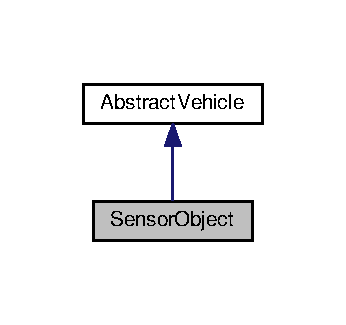
\includegraphics[width=166pt]{classSensorObject__inherit__graph}
\end{center}
\end{figure}


Collaboration diagram for Sensor\+Object\+:\nopagebreak
\begin{figure}[H]
\begin{center}
\leavevmode
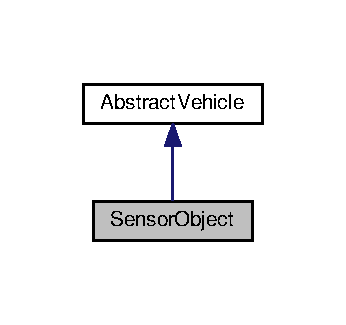
\includegraphics[width=166pt]{classSensorObject__coll__graph}
\end{center}
\end{figure}
\subsection*{Public Member Functions}
\begin{DoxyCompactItemize}
\item 
\hyperlink{classSensorObject_ac4ac2559d3fbe122bd585860d19f54a8}{Sensor\+Object} ()
\item 
double \hyperlink{classSensorObject_ab3e8516fb8273082efbc873266667486}{get\+Speed} ()
\item 
double \hyperlink{classSensorObject_abcd7baf59194b7fef7d0ec75eb880123}{get\+Speed\+\_\+x} ()
\item 
double \hyperlink{classSensorObject_a0fcc2d7351b630b61fbd5395ac568bc4}{get\+Speed\+\_\+y} ()
\item 
string \hyperlink{classSensorObject_adaa7350730c3c627f0f215c251386cb7}{display} ()
\item 
void \hyperlink{classSensorObject_a4d0023c0d36c15df10aade6ec224cc56}{update} (\hyperlink{main_8cpp_ab701e3ac61a85b337ec5c1abaad6742d}{json} j)
\item 
vector$<$ double $>$ \hyperlink{classSensorObject_a49714af72f563ce1114c9f43e95d7af8}{get\+Prediction} (int second)
\item 
void \hyperlink{classSensorObject_a6787ced615e75d519842ab2e893048ca}{calculate\+Predictions} (int prediction\+Horizon)
\end{DoxyCompactItemize}
\subsection*{Protected Member Functions}
\begin{DoxyCompactItemize}
\item 
double \hyperlink{classSensorObject_ad11229216ab0dcbbe82aaa9454720255}{get\+Probability\+Of\+Lane\+Change\+Left} ()
\item 
double \hyperlink{classSensorObject_a132c4fa7451f21b328bf8252e84fe823}{get\+Probability\+Of\+Lane\+Change\+Right} ()
\item 
double \hyperlink{classSensorObject_a3cae3fdbe83f10c4c308c1dc68540cd1}{get\+Probability\+Of\+Lane\+Keep} ()
\end{DoxyCompactItemize}
\subsection*{Protected Attributes}
\begin{DoxyCompactItemize}
\item 
double \hyperlink{classSensorObject_ae33a03dcbff51436ce91dbdc8c27f4b3}{speed\+\_\+x}
\item 
double \hyperlink{classSensorObject_aa5fa4bb2ebea9261cdb80b0ef31cb386}{speed\+\_\+y}
\end{DoxyCompactItemize}


\subsection{Constructor \& Destructor Documentation}
\index{Sensor\+Object@{Sensor\+Object}!Sensor\+Object@{Sensor\+Object}}
\index{Sensor\+Object@{Sensor\+Object}!Sensor\+Object@{Sensor\+Object}}
\subsubsection[{\texorpdfstring{Sensor\+Object()}{SensorObject()}}]{\setlength{\rightskip}{0pt plus 5cm}Sensor\+Object\+::\+Sensor\+Object (
\begin{DoxyParamCaption}
{}
\end{DoxyParamCaption}
)}\hypertarget{classSensorObject_ac4ac2559d3fbe122bd585860d19f54a8}{}\label{classSensorObject_ac4ac2559d3fbe122bd585860d19f54a8}


\subsection{Member Function Documentation}
\index{Sensor\+Object@{Sensor\+Object}!calculate\+Predictions@{calculate\+Predictions}}
\index{calculate\+Predictions@{calculate\+Predictions}!Sensor\+Object@{Sensor\+Object}}
\subsubsection[{\texorpdfstring{calculate\+Predictions(int prediction\+Horizon)}{calculatePredictions(int predictionHorizon)}}]{\setlength{\rightskip}{0pt plus 5cm}void Sensor\+Object\+::calculate\+Predictions (
\begin{DoxyParamCaption}
\item[{int}]{prediction\+Horizon}
\end{DoxyParamCaption}
)\hspace{0.3cm}{\ttfamily [virtual]}}\hypertarget{classSensorObject_a6787ced615e75d519842ab2e893048ca}{}\label{classSensorObject_a6787ced615e75d519842ab2e893048ca}


Implements \hyperlink{classAbstractVehicle_a631115b44756050ccf2a7fe975787035}{Abstract\+Vehicle}.

\index{Sensor\+Object@{Sensor\+Object}!display@{display}}
\index{display@{display}!Sensor\+Object@{Sensor\+Object}}
\subsubsection[{\texorpdfstring{display()}{display()}}]{\setlength{\rightskip}{0pt plus 5cm}string Sensor\+Object\+::display (
\begin{DoxyParamCaption}
{}
\end{DoxyParamCaption}
)\hspace{0.3cm}{\ttfamily [virtual]}}\hypertarget{classSensorObject_adaa7350730c3c627f0f215c251386cb7}{}\label{classSensorObject_adaa7350730c3c627f0f215c251386cb7}


Implements \hyperlink{classAbstractVehicle_ada311ec475179ba776966f7e3ddcb91a}{Abstract\+Vehicle}.



Here is the call graph for this function\+:\nopagebreak
\begin{figure}[H]
\begin{center}
\leavevmode
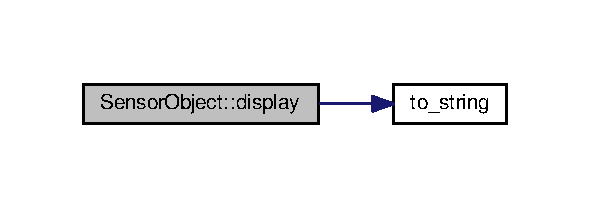
\includegraphics[width=283pt]{classSensorObject_adaa7350730c3c627f0f215c251386cb7_cgraph}
\end{center}
\end{figure}


\index{Sensor\+Object@{Sensor\+Object}!get\+Prediction@{get\+Prediction}}
\index{get\+Prediction@{get\+Prediction}!Sensor\+Object@{Sensor\+Object}}
\subsubsection[{\texorpdfstring{get\+Prediction(int second)}{getPrediction(int second)}}]{\setlength{\rightskip}{0pt plus 5cm}vector$<$ double $>$ Sensor\+Object\+::get\+Prediction (
\begin{DoxyParamCaption}
\item[{int}]{second}
\end{DoxyParamCaption}
)\hspace{0.3cm}{\ttfamily [virtual]}}\hypertarget{classSensorObject_a49714af72f563ce1114c9f43e95d7af8}{}\label{classSensorObject_a49714af72f563ce1114c9f43e95d7af8}


Implements \hyperlink{classAbstractVehicle_a3c84d6970c9461bfafd76cf48d6bece0}{Abstract\+Vehicle}.

\index{Sensor\+Object@{Sensor\+Object}!get\+Probability\+Of\+Lane\+Change\+Left@{get\+Probability\+Of\+Lane\+Change\+Left}}
\index{get\+Probability\+Of\+Lane\+Change\+Left@{get\+Probability\+Of\+Lane\+Change\+Left}!Sensor\+Object@{Sensor\+Object}}
\subsubsection[{\texorpdfstring{get\+Probability\+Of\+Lane\+Change\+Left()}{getProbabilityOfLaneChangeLeft()}}]{\setlength{\rightskip}{0pt plus 5cm}double Sensor\+Object\+::get\+Probability\+Of\+Lane\+Change\+Left (
\begin{DoxyParamCaption}
{}
\end{DoxyParamCaption}
)\hspace{0.3cm}{\ttfamily [protected]}}\hypertarget{classSensorObject_ad11229216ab0dcbbe82aaa9454720255}{}\label{classSensorObject_ad11229216ab0dcbbe82aaa9454720255}
\index{Sensor\+Object@{Sensor\+Object}!get\+Probability\+Of\+Lane\+Change\+Right@{get\+Probability\+Of\+Lane\+Change\+Right}}
\index{get\+Probability\+Of\+Lane\+Change\+Right@{get\+Probability\+Of\+Lane\+Change\+Right}!Sensor\+Object@{Sensor\+Object}}
\subsubsection[{\texorpdfstring{get\+Probability\+Of\+Lane\+Change\+Right()}{getProbabilityOfLaneChangeRight()}}]{\setlength{\rightskip}{0pt plus 5cm}double Sensor\+Object\+::get\+Probability\+Of\+Lane\+Change\+Right (
\begin{DoxyParamCaption}
{}
\end{DoxyParamCaption}
)\hspace{0.3cm}{\ttfamily [protected]}}\hypertarget{classSensorObject_a132c4fa7451f21b328bf8252e84fe823}{}\label{classSensorObject_a132c4fa7451f21b328bf8252e84fe823}
\index{Sensor\+Object@{Sensor\+Object}!get\+Probability\+Of\+Lane\+Keep@{get\+Probability\+Of\+Lane\+Keep}}
\index{get\+Probability\+Of\+Lane\+Keep@{get\+Probability\+Of\+Lane\+Keep}!Sensor\+Object@{Sensor\+Object}}
\subsubsection[{\texorpdfstring{get\+Probability\+Of\+Lane\+Keep()}{getProbabilityOfLaneKeep()}}]{\setlength{\rightskip}{0pt plus 5cm}double Sensor\+Object\+::get\+Probability\+Of\+Lane\+Keep (
\begin{DoxyParamCaption}
{}
\end{DoxyParamCaption}
)\hspace{0.3cm}{\ttfamily [protected]}}\hypertarget{classSensorObject_a3cae3fdbe83f10c4c308c1dc68540cd1}{}\label{classSensorObject_a3cae3fdbe83f10c4c308c1dc68540cd1}
\index{Sensor\+Object@{Sensor\+Object}!get\+Speed@{get\+Speed}}
\index{get\+Speed@{get\+Speed}!Sensor\+Object@{Sensor\+Object}}
\subsubsection[{\texorpdfstring{get\+Speed()}{getSpeed()}}]{\setlength{\rightskip}{0pt plus 5cm}double Sensor\+Object\+::get\+Speed (
\begin{DoxyParamCaption}
{}
\end{DoxyParamCaption}
)\hspace{0.3cm}{\ttfamily [virtual]}}\hypertarget{classSensorObject_ab3e8516fb8273082efbc873266667486}{}\label{classSensorObject_ab3e8516fb8273082efbc873266667486}


Implements \hyperlink{classAbstractVehicle_a17c193d56e1da24a1008ae52859d31c7}{Abstract\+Vehicle}.

\index{Sensor\+Object@{Sensor\+Object}!get\+Speed\+\_\+x@{get\+Speed\+\_\+x}}
\index{get\+Speed\+\_\+x@{get\+Speed\+\_\+x}!Sensor\+Object@{Sensor\+Object}}
\subsubsection[{\texorpdfstring{get\+Speed\+\_\+x()}{getSpeed_x()}}]{\setlength{\rightskip}{0pt plus 5cm}double Sensor\+Object\+::get\+Speed\+\_\+x (
\begin{DoxyParamCaption}
{}
\end{DoxyParamCaption}
)\hspace{0.3cm}{\ttfamily [virtual]}}\hypertarget{classSensorObject_abcd7baf59194b7fef7d0ec75eb880123}{}\label{classSensorObject_abcd7baf59194b7fef7d0ec75eb880123}


Implements \hyperlink{classAbstractVehicle_abe9a9f5e2290fdf4207ac0206b9e97a3}{Abstract\+Vehicle}.

\index{Sensor\+Object@{Sensor\+Object}!get\+Speed\+\_\+y@{get\+Speed\+\_\+y}}
\index{get\+Speed\+\_\+y@{get\+Speed\+\_\+y}!Sensor\+Object@{Sensor\+Object}}
\subsubsection[{\texorpdfstring{get\+Speed\+\_\+y()}{getSpeed_y()}}]{\setlength{\rightskip}{0pt plus 5cm}double Sensor\+Object\+::get\+Speed\+\_\+y (
\begin{DoxyParamCaption}
{}
\end{DoxyParamCaption}
)\hspace{0.3cm}{\ttfamily [virtual]}}\hypertarget{classSensorObject_a0fcc2d7351b630b61fbd5395ac568bc4}{}\label{classSensorObject_a0fcc2d7351b630b61fbd5395ac568bc4}


Implements \hyperlink{classAbstractVehicle_a90e6e4299070bace1acfd8d79bf78c95}{Abstract\+Vehicle}.

\index{Sensor\+Object@{Sensor\+Object}!update@{update}}
\index{update@{update}!Sensor\+Object@{Sensor\+Object}}
\subsubsection[{\texorpdfstring{update(json j)}{update(json j)}}]{\setlength{\rightskip}{0pt plus 5cm}void Sensor\+Object\+::update (
\begin{DoxyParamCaption}
\item[{{\bf json}}]{j}
\end{DoxyParamCaption}
)\hspace{0.3cm}{\ttfamily [virtual]}}\hypertarget{classSensorObject_a4d0023c0d36c15df10aade6ec224cc56}{}\label{classSensorObject_a4d0023c0d36c15df10aade6ec224cc56}


Implements \hyperlink{classAbstractVehicle_a004b43b4a4d02ca6122ed8862c672de3}{Abstract\+Vehicle}.



Here is the call graph for this function\+:\nopagebreak
\begin{figure}[H]
\begin{center}
\leavevmode
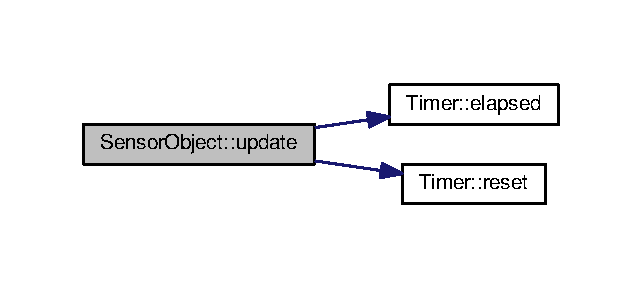
\includegraphics[width=308pt]{classSensorObject_a4d0023c0d36c15df10aade6ec224cc56_cgraph}
\end{center}
\end{figure}




\subsection{Member Data Documentation}
\index{Sensor\+Object@{Sensor\+Object}!speed\+\_\+x@{speed\+\_\+x}}
\index{speed\+\_\+x@{speed\+\_\+x}!Sensor\+Object@{Sensor\+Object}}
\subsubsection[{\texorpdfstring{speed\+\_\+x}{speed_x}}]{\setlength{\rightskip}{0pt plus 5cm}double Sensor\+Object\+::speed\+\_\+x\hspace{0.3cm}{\ttfamily [protected]}}\hypertarget{classSensorObject_ae33a03dcbff51436ce91dbdc8c27f4b3}{}\label{classSensorObject_ae33a03dcbff51436ce91dbdc8c27f4b3}
\index{Sensor\+Object@{Sensor\+Object}!speed\+\_\+y@{speed\+\_\+y}}
\index{speed\+\_\+y@{speed\+\_\+y}!Sensor\+Object@{Sensor\+Object}}
\subsubsection[{\texorpdfstring{speed\+\_\+y}{speed_y}}]{\setlength{\rightskip}{0pt plus 5cm}double Sensor\+Object\+::speed\+\_\+y\hspace{0.3cm}{\ttfamily [protected]}}\hypertarget{classSensorObject_aa5fa4bb2ebea9261cdb80b0ef31cb386}{}\label{classSensorObject_aa5fa4bb2ebea9261cdb80b0ef31cb386}


The documentation for this class was generated from the following files\+:\begin{DoxyCompactItemize}
\item 
src/\hyperlink{SensorObject_8h}{Sensor\+Object.\+h}\item 
src/\hyperlink{SensorObject_8cpp}{Sensor\+Object.\+cpp}\end{DoxyCompactItemize}

\hypertarget{classTimer}{}\section{Timer Class Reference}
\label{classTimer}\index{Timer@{Timer}}


{\ttfamily \#include $<$helper.\+h$>$}

\subsection*{Public Member Functions}
\begin{DoxyCompactItemize}
\item 
\hyperlink{classTimer_a5f16e8da27d2a5a5242dead46de05d97}{Timer} ()
\item 
void \hyperlink{classTimer_a9020542d73357a4eef512eefaf57524b}{reset} ()
\item 
double \hyperlink{classTimer_a69004f2e48f639d17e82abe340c4819a}{elapsed} () const 
\end{DoxyCompactItemize}


\subsection{Constructor \& Destructor Documentation}
\index{Timer@{Timer}!Timer@{Timer}}
\index{Timer@{Timer}!Timer@{Timer}}
\subsubsection[{\texorpdfstring{Timer()}{Timer()}}]{\setlength{\rightskip}{0pt plus 5cm}Timer\+::\+Timer (
\begin{DoxyParamCaption}
{}
\end{DoxyParamCaption}
)\hspace{0.3cm}{\ttfamily [inline]}}\hypertarget{classTimer_a5f16e8da27d2a5a5242dead46de05d97}{}\label{classTimer_a5f16e8da27d2a5a5242dead46de05d97}


\subsection{Member Function Documentation}
\index{Timer@{Timer}!elapsed@{elapsed}}
\index{elapsed@{elapsed}!Timer@{Timer}}
\subsubsection[{\texorpdfstring{elapsed() const }{elapsed() const }}]{\setlength{\rightskip}{0pt plus 5cm}double Timer\+::elapsed (
\begin{DoxyParamCaption}
{}
\end{DoxyParamCaption}
) const\hspace{0.3cm}{\ttfamily [inline]}}\hypertarget{classTimer_a69004f2e48f639d17e82abe340c4819a}{}\label{classTimer_a69004f2e48f639d17e82abe340c4819a}
\index{Timer@{Timer}!reset@{reset}}
\index{reset@{reset}!Timer@{Timer}}
\subsubsection[{\texorpdfstring{reset()}{reset()}}]{\setlength{\rightskip}{0pt plus 5cm}void Timer\+::reset (
\begin{DoxyParamCaption}
{}
\end{DoxyParamCaption}
)\hspace{0.3cm}{\ttfamily [inline]}}\hypertarget{classTimer_a9020542d73357a4eef512eefaf57524b}{}\label{classTimer_a9020542d73357a4eef512eefaf57524b}


The documentation for this class was generated from the following file\+:\begin{DoxyCompactItemize}
\item 
src/\hyperlink{helper_8h}{helper.\+h}\end{DoxyCompactItemize}

\hypertarget{classTrajectoryPlanner}{}\section{Trajectory\+Planner Class Reference}
\label{classTrajectoryPlanner}\index{Trajectory\+Planner@{Trajectory\+Planner}}


{\ttfamily \#include $<$Trajectory\+Planner.\+h$>$}

\subsection*{Public Member Functions}
\begin{DoxyCompactItemize}
\item 
void \hyperlink{classTrajectoryPlanner_ae59e35b4d9fce61283412ab099d94f66}{load\+Map} ()
\item 
vector$<$ vector$<$ double $>$ $>$ \hyperlink{classTrajectoryPlanner_a046a79f994d48d6ac2c5db82a9100512}{calc\+Traj\+From\+QA} (\hyperlink{classEgoVehicle}{Ego\+Vehicle} ego\+Vehicle, double target\+\_\+speed, int target\+\_\+lane)
\end{DoxyCompactItemize}
\subsection*{Protected Member Functions}
\begin{DoxyCompactItemize}
\item 
vector$<$ double $>$ \hyperlink{classTrajectoryPlanner_ae7510d0c40770043b10cc6e6d83a857c}{get\+Frenet} (double x, double y)
\item 
vector$<$ double $>$ \hyperlink{classTrajectoryPlanner_a8469f790a9a144901d1bf9d533865067}{get\+XY} (double s, double d)
\item 
int \hyperlink{classTrajectoryPlanner_a431693acbdb03af68dab2dff8fb236a3}{Next\+Waypoint} (double x, double y)
\item 
int \hyperlink{classTrajectoryPlanner_ad43e018e594d61eadae5e6bad49c4334}{Closest\+Waypoint} (double x, double y)
\end{DoxyCompactItemize}
\subsection*{Protected Attributes}
\begin{DoxyCompactItemize}
\item 
string \hyperlink{classTrajectoryPlanner_a42fcd2cde1df11a1d024163c5128324e}{map\+\_\+file\+\_\+} = \char`\"{}../data/highway\+\_\+map.\+csv\char`\"{}
\item 
double \hyperlink{classTrajectoryPlanner_ae0aef5ddc2586b021db0200812fcf72d}{max\+\_\+s} = 6945.\+554
\item 
vector$<$ double $>$ \hyperlink{classTrajectoryPlanner_a1b07d4fa7c5b7567b0ee2f3d1dad16ab}{maps\+\_\+x}
\item 
vector$<$ double $>$ \hyperlink{classTrajectoryPlanner_a95195c80ec4a38d10fb70bff4ad0a6bc}{maps\+\_\+y}
\item 
vector$<$ double $>$ \hyperlink{classTrajectoryPlanner_acf24bbd43d3d607c186cc26585063cc3}{maps\+\_\+s}
\item 
vector$<$ double $>$ \hyperlink{classTrajectoryPlanner_abc73d54d380e2f17933badebc66f0b3f}{maps\+\_\+dx}
\item 
vector$<$ double $>$ \hyperlink{classTrajectoryPlanner_a937323d974a19a86ff6792c663c6eb53}{maps\+\_\+dy}
\end{DoxyCompactItemize}


\subsection{Member Function Documentation}
\index{Trajectory\+Planner@{Trajectory\+Planner}!calc\+Traj\+From\+QA@{calc\+Traj\+From\+QA}}
\index{calc\+Traj\+From\+QA@{calc\+Traj\+From\+QA}!Trajectory\+Planner@{Trajectory\+Planner}}
\subsubsection[{\texorpdfstring{calc\+Traj\+From\+Q\+A(\+Ego\+Vehicle ego\+Vehicle, double target\+\_\+speed, int target\+\_\+lane)}{calcTrajFromQA(EgoVehicle egoVehicle, double target_speed, int target_lane)}}]{\setlength{\rightskip}{0pt plus 5cm}vector$<$ vector$<$ double $>$ $>$ Trajectory\+Planner\+::calc\+Traj\+From\+QA (
\begin{DoxyParamCaption}
\item[{{\bf Ego\+Vehicle}}]{ego\+Vehicle, }
\item[{double}]{target\+\_\+speed, }
\item[{int}]{target\+\_\+lane}
\end{DoxyParamCaption}
)}\hypertarget{classTrajectoryPlanner_a046a79f994d48d6ac2c5db82a9100512}{}\label{classTrajectoryPlanner_a046a79f994d48d6ac2c5db82a9100512}


Here is the call graph for this function\+:\nopagebreak
\begin{figure}[H]
\begin{center}
\leavevmode
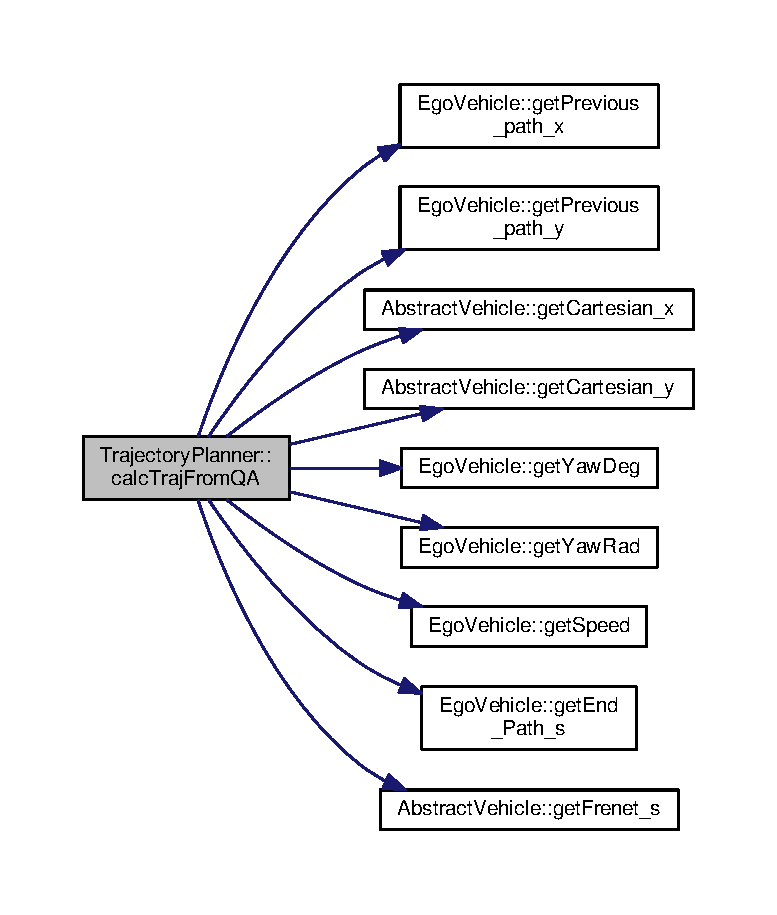
\includegraphics[width=350pt]{classTrajectoryPlanner_a046a79f994d48d6ac2c5db82a9100512_cgraph}
\end{center}
\end{figure}


\index{Trajectory\+Planner@{Trajectory\+Planner}!Closest\+Waypoint@{Closest\+Waypoint}}
\index{Closest\+Waypoint@{Closest\+Waypoint}!Trajectory\+Planner@{Trajectory\+Planner}}
\subsubsection[{\texorpdfstring{Closest\+Waypoint(double x, double y)}{ClosestWaypoint(double x, double y)}}]{\setlength{\rightskip}{0pt plus 5cm}int Trajectory\+Planner\+::\+Closest\+Waypoint (
\begin{DoxyParamCaption}
\item[{double}]{x, }
\item[{double}]{y}
\end{DoxyParamCaption}
)\hspace{0.3cm}{\ttfamily [protected]}}\hypertarget{classTrajectoryPlanner_ad43e018e594d61eadae5e6bad49c4334}{}\label{classTrajectoryPlanner_ad43e018e594d61eadae5e6bad49c4334}


Here is the call graph for this function\+:\nopagebreak
\begin{figure}[H]
\begin{center}
\leavevmode
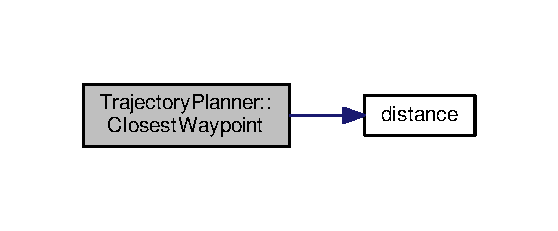
\includegraphics[width=268pt]{classTrajectoryPlanner_ad43e018e594d61eadae5e6bad49c4334_cgraph}
\end{center}
\end{figure}


\index{Trajectory\+Planner@{Trajectory\+Planner}!get\+Frenet@{get\+Frenet}}
\index{get\+Frenet@{get\+Frenet}!Trajectory\+Planner@{Trajectory\+Planner}}
\subsubsection[{\texorpdfstring{get\+Frenet(double x, double y)}{getFrenet(double x, double y)}}]{\setlength{\rightskip}{0pt plus 5cm}vector$<$ double $>$ Trajectory\+Planner\+::get\+Frenet (
\begin{DoxyParamCaption}
\item[{double}]{x, }
\item[{double}]{y}
\end{DoxyParamCaption}
)\hspace{0.3cm}{\ttfamily [protected]}}\hypertarget{classTrajectoryPlanner_ae7510d0c40770043b10cc6e6d83a857c}{}\label{classTrajectoryPlanner_ae7510d0c40770043b10cc6e6d83a857c}


Here is the call graph for this function\+:\nopagebreak
\begin{figure}[H]
\begin{center}
\leavevmode
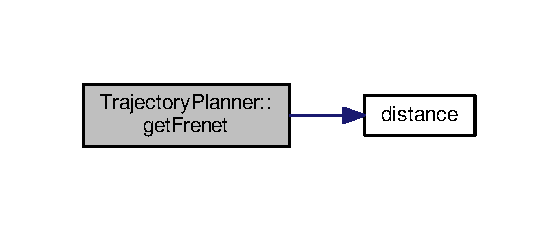
\includegraphics[width=268pt]{classTrajectoryPlanner_ae7510d0c40770043b10cc6e6d83a857c_cgraph}
\end{center}
\end{figure}


\index{Trajectory\+Planner@{Trajectory\+Planner}!get\+XY@{get\+XY}}
\index{get\+XY@{get\+XY}!Trajectory\+Planner@{Trajectory\+Planner}}
\subsubsection[{\texorpdfstring{get\+X\+Y(double s, double d)}{getXY(double s, double d)}}]{\setlength{\rightskip}{0pt plus 5cm}vector$<$ double $>$ Trajectory\+Planner\+::get\+XY (
\begin{DoxyParamCaption}
\item[{double}]{s, }
\item[{double}]{d}
\end{DoxyParamCaption}
)\hspace{0.3cm}{\ttfamily [protected]}}\hypertarget{classTrajectoryPlanner_a8469f790a9a144901d1bf9d533865067}{}\label{classTrajectoryPlanner_a8469f790a9a144901d1bf9d533865067}


Here is the call graph for this function\+:\nopagebreak
\begin{figure}[H]
\begin{center}
\leavevmode
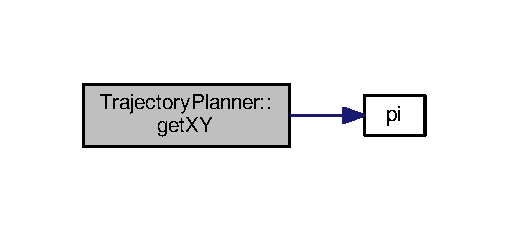
\includegraphics[width=244pt]{classTrajectoryPlanner_a8469f790a9a144901d1bf9d533865067_cgraph}
\end{center}
\end{figure}


\index{Trajectory\+Planner@{Trajectory\+Planner}!load\+Map@{load\+Map}}
\index{load\+Map@{load\+Map}!Trajectory\+Planner@{Trajectory\+Planner}}
\subsubsection[{\texorpdfstring{load\+Map()}{loadMap()}}]{\setlength{\rightskip}{0pt plus 5cm}void Trajectory\+Planner\+::load\+Map (
\begin{DoxyParamCaption}
{}
\end{DoxyParamCaption}
)}\hypertarget{classTrajectoryPlanner_ae59e35b4d9fce61283412ab099d94f66}{}\label{classTrajectoryPlanner_ae59e35b4d9fce61283412ab099d94f66}
\index{Trajectory\+Planner@{Trajectory\+Planner}!Next\+Waypoint@{Next\+Waypoint}}
\index{Next\+Waypoint@{Next\+Waypoint}!Trajectory\+Planner@{Trajectory\+Planner}}
\subsubsection[{\texorpdfstring{Next\+Waypoint(double x, double y)}{NextWaypoint(double x, double y)}}]{\setlength{\rightskip}{0pt plus 5cm}int Trajectory\+Planner\+::\+Next\+Waypoint (
\begin{DoxyParamCaption}
\item[{double}]{x, }
\item[{double}]{y}
\end{DoxyParamCaption}
)\hspace{0.3cm}{\ttfamily [protected]}}\hypertarget{classTrajectoryPlanner_a431693acbdb03af68dab2dff8fb236a3}{}\label{classTrajectoryPlanner_a431693acbdb03af68dab2dff8fb236a3}


\subsection{Member Data Documentation}
\index{Trajectory\+Planner@{Trajectory\+Planner}!map\+\_\+file\+\_\+@{map\+\_\+file\+\_\+}}
\index{map\+\_\+file\+\_\+@{map\+\_\+file\+\_\+}!Trajectory\+Planner@{Trajectory\+Planner}}
\subsubsection[{\texorpdfstring{map\+\_\+file\+\_\+}{map_file_}}]{\setlength{\rightskip}{0pt plus 5cm}string Trajectory\+Planner\+::map\+\_\+file\+\_\+ = \char`\"{}../data/highway\+\_\+map.\+csv\char`\"{}\hspace{0.3cm}{\ttfamily [protected]}}\hypertarget{classTrajectoryPlanner_a42fcd2cde1df11a1d024163c5128324e}{}\label{classTrajectoryPlanner_a42fcd2cde1df11a1d024163c5128324e}
\index{Trajectory\+Planner@{Trajectory\+Planner}!maps\+\_\+dx@{maps\+\_\+dx}}
\index{maps\+\_\+dx@{maps\+\_\+dx}!Trajectory\+Planner@{Trajectory\+Planner}}
\subsubsection[{\texorpdfstring{maps\+\_\+dx}{maps_dx}}]{\setlength{\rightskip}{0pt plus 5cm}vector$<$double$>$ Trajectory\+Planner\+::maps\+\_\+dx\hspace{0.3cm}{\ttfamily [protected]}}\hypertarget{classTrajectoryPlanner_abc73d54d380e2f17933badebc66f0b3f}{}\label{classTrajectoryPlanner_abc73d54d380e2f17933badebc66f0b3f}
\index{Trajectory\+Planner@{Trajectory\+Planner}!maps\+\_\+dy@{maps\+\_\+dy}}
\index{maps\+\_\+dy@{maps\+\_\+dy}!Trajectory\+Planner@{Trajectory\+Planner}}
\subsubsection[{\texorpdfstring{maps\+\_\+dy}{maps_dy}}]{\setlength{\rightskip}{0pt plus 5cm}vector$<$double$>$ Trajectory\+Planner\+::maps\+\_\+dy\hspace{0.3cm}{\ttfamily [protected]}}\hypertarget{classTrajectoryPlanner_a937323d974a19a86ff6792c663c6eb53}{}\label{classTrajectoryPlanner_a937323d974a19a86ff6792c663c6eb53}
\index{Trajectory\+Planner@{Trajectory\+Planner}!maps\+\_\+s@{maps\+\_\+s}}
\index{maps\+\_\+s@{maps\+\_\+s}!Trajectory\+Planner@{Trajectory\+Planner}}
\subsubsection[{\texorpdfstring{maps\+\_\+s}{maps_s}}]{\setlength{\rightskip}{0pt plus 5cm}vector$<$double$>$ Trajectory\+Planner\+::maps\+\_\+s\hspace{0.3cm}{\ttfamily [protected]}}\hypertarget{classTrajectoryPlanner_acf24bbd43d3d607c186cc26585063cc3}{}\label{classTrajectoryPlanner_acf24bbd43d3d607c186cc26585063cc3}
\index{Trajectory\+Planner@{Trajectory\+Planner}!maps\+\_\+x@{maps\+\_\+x}}
\index{maps\+\_\+x@{maps\+\_\+x}!Trajectory\+Planner@{Trajectory\+Planner}}
\subsubsection[{\texorpdfstring{maps\+\_\+x}{maps_x}}]{\setlength{\rightskip}{0pt plus 5cm}vector$<$double$>$ Trajectory\+Planner\+::maps\+\_\+x\hspace{0.3cm}{\ttfamily [protected]}}\hypertarget{classTrajectoryPlanner_a1b07d4fa7c5b7567b0ee2f3d1dad16ab}{}\label{classTrajectoryPlanner_a1b07d4fa7c5b7567b0ee2f3d1dad16ab}
\index{Trajectory\+Planner@{Trajectory\+Planner}!maps\+\_\+y@{maps\+\_\+y}}
\index{maps\+\_\+y@{maps\+\_\+y}!Trajectory\+Planner@{Trajectory\+Planner}}
\subsubsection[{\texorpdfstring{maps\+\_\+y}{maps_y}}]{\setlength{\rightskip}{0pt plus 5cm}vector$<$double$>$ Trajectory\+Planner\+::maps\+\_\+y\hspace{0.3cm}{\ttfamily [protected]}}\hypertarget{classTrajectoryPlanner_a95195c80ec4a38d10fb70bff4ad0a6bc}{}\label{classTrajectoryPlanner_a95195c80ec4a38d10fb70bff4ad0a6bc}
\index{Trajectory\+Planner@{Trajectory\+Planner}!max\+\_\+s@{max\+\_\+s}}
\index{max\+\_\+s@{max\+\_\+s}!Trajectory\+Planner@{Trajectory\+Planner}}
\subsubsection[{\texorpdfstring{max\+\_\+s}{max_s}}]{\setlength{\rightskip}{0pt plus 5cm}double Trajectory\+Planner\+::max\+\_\+s = 6945.\+554\hspace{0.3cm}{\ttfamily [protected]}}\hypertarget{classTrajectoryPlanner_ae0aef5ddc2586b021db0200812fcf72d}{}\label{classTrajectoryPlanner_ae0aef5ddc2586b021db0200812fcf72d}


The documentation for this class was generated from the following files\+:\begin{DoxyCompactItemize}
\item 
src/\hyperlink{TrajectoryPlanner_8h}{Trajectory\+Planner.\+h}\item 
src/\hyperlink{TrajectoryPlanner_8cpp}{Trajectory\+Planner.\+cpp}\end{DoxyCompactItemize}

\hypertarget{classTrajectoryPlannerWIP}{}\section{Trajectory\+Planner\+W\+IP Class Reference}
\label{classTrajectoryPlannerWIP}\index{Trajectory\+Planner\+W\+IP@{Trajectory\+Planner\+W\+IP}}


{\ttfamily \#include $<$Trajectory\+Planner\+W\+I\+P.\+h$>$}

\subsection*{Public Member Functions}
\begin{DoxyCompactItemize}
\item 
void \hyperlink{classTrajectoryPlannerWIP_ae13818910d1d7b7a65eacf49ebd1682d}{load\+Map} ()
\item 
vector$<$ vector$<$ double $>$ $>$ \hyperlink{classTrajectoryPlannerWIP_a9c53694540c32d1e724def363c20d310}{get\+Next\+Path\+Trajectory} (double start\+\_\+s, double start\+\_\+d, double target\+\_\+lane, double current\+\_\+speed, double ref\+\_\+speed, double Time)
\item 
vector$<$ vector$<$ double $>$ $>$ \hyperlink{classTrajectoryPlannerWIP_aeb7dc782540b1e43b7be2f7075d23b75}{merge\+Trajectories} (vector$<$ double $>$ \hyperlink{classTrajectoryPlannerWIP_a74997cfa081e6d4409d4d2234e5b3855}{previous\+\_\+path\+\_\+x}, vector$<$ double $>$ \hyperlink{classTrajectoryPlannerWIP_a32a8ed201b7abf6a5817e17ba5e4fca3}{previous\+\_\+path\+\_\+y}, double \hyperlink{classTrajectoryPlannerWIP_a1239028b8c1d13c6e03237f160965112}{end\+\_\+path\+\_\+s}, double \hyperlink{classTrajectoryPlannerWIP_a45a0c4e41dae17e9387b358d472bdb55}{end\+\_\+path\+\_\+d}, vector$<$ vector$<$ double $>$$>$ new\+Traj)
\end{DoxyCompactItemize}
\subsection*{Public Attributes}
\begin{DoxyCompactItemize}
\item 
vector$<$ double $>$ \hyperlink{classTrajectoryPlannerWIP_a74997cfa081e6d4409d4d2234e5b3855}{previous\+\_\+path\+\_\+x}
\item 
vector$<$ double $>$ \hyperlink{classTrajectoryPlannerWIP_a32a8ed201b7abf6a5817e17ba5e4fca3}{previous\+\_\+path\+\_\+y}
\item 
double \hyperlink{classTrajectoryPlannerWIP_a1239028b8c1d13c6e03237f160965112}{end\+\_\+path\+\_\+s}
\item 
double \hyperlink{classTrajectoryPlannerWIP_a45a0c4e41dae17e9387b358d472bdb55}{end\+\_\+path\+\_\+d}
\end{DoxyCompactItemize}
\subsection*{Protected Member Functions}
\begin{DoxyCompactItemize}
\item 
vector$<$ double $>$ \hyperlink{classTrajectoryPlannerWIP_a90ba8175932f377a2f56795edb8eb1eb}{get\+Frenet} (double x, double y)
\item 
vector$<$ double $>$ \hyperlink{classTrajectoryPlannerWIP_a6c4a03d5e4f4b78bdbd91debe2d1b246}{get\+XY} (double s, double d)
\item 
vector$<$ double $>$ \hyperlink{classTrajectoryPlannerWIP_ac2053a967111d1f776616ea7a473cfa0}{J\+MT} (vector$<$ double $>$ start, vector$<$ double $>$ end, double T)
\item 
vector$<$ double $>$ \hyperlink{classTrajectoryPlannerWIP_a836cd57fcddc08790c6c4a33249e3161}{predict\+Next\+Endpoint} (double start\+\_\+s, double start\+\_\+d, double lane, double current\+\_\+speed, double ref\+\_\+speed, double Time)
\item 
int \hyperlink{classTrajectoryPlannerWIP_afcec4651796ba110751bddeb25f223fa}{Next\+Waypoint} (double x, double y)
\item 
int \hyperlink{classTrajectoryPlannerWIP_a9f787291e9065422a9c649c6b24acf8e}{Closest\+Waypoint} (double x, double y)
\end{DoxyCompactItemize}
\subsection*{Protected Attributes}
\begin{DoxyCompactItemize}
\item 
string \hyperlink{classTrajectoryPlannerWIP_a87aa1ae8bce8788c8fab3db76b92997c}{map\+\_\+file\+\_\+} = \char`\"{}../data/highway\+\_\+map.\+csv\char`\"{}
\item 
double \hyperlink{classTrajectoryPlannerWIP_a43501cae77daf85f811ed0873d9bf960}{max\+\_\+s} = 6945.\+554
\item 
vector$<$ double $>$ \hyperlink{classTrajectoryPlannerWIP_abaa6f54058eb01c7c16df360c6883496}{maps\+\_\+x}
\item 
vector$<$ double $>$ \hyperlink{classTrajectoryPlannerWIP_a17cfcc4b66e5fff8a1802e5fc9dd7639}{maps\+\_\+y}
\item 
vector$<$ double $>$ \hyperlink{classTrajectoryPlannerWIP_a38af64be0ca058c3ac72d6cf2883de9f}{maps\+\_\+s}
\item 
vector$<$ double $>$ \hyperlink{classTrajectoryPlannerWIP_a60657fd8df138c58a1a9333f07f73f7e}{maps\+\_\+dx}
\item 
vector$<$ double $>$ \hyperlink{classTrajectoryPlannerWIP_ae1fd51251d18023cc395eff388785b13}{maps\+\_\+dy}
\end{DoxyCompactItemize}


\subsection{Member Function Documentation}
\index{Trajectory\+Planner\+W\+IP@{Trajectory\+Planner\+W\+IP}!Closest\+Waypoint@{Closest\+Waypoint}}
\index{Closest\+Waypoint@{Closest\+Waypoint}!Trajectory\+Planner\+W\+IP@{Trajectory\+Planner\+W\+IP}}
\subsubsection[{\texorpdfstring{Closest\+Waypoint(double x, double y)}{ClosestWaypoint(double x, double y)}}]{\setlength{\rightskip}{0pt plus 5cm}int Trajectory\+Planner\+W\+I\+P\+::\+Closest\+Waypoint (
\begin{DoxyParamCaption}
\item[{double}]{x, }
\item[{double}]{y}
\end{DoxyParamCaption}
)\hspace{0.3cm}{\ttfamily [protected]}}\hypertarget{classTrajectoryPlannerWIP_a9f787291e9065422a9c649c6b24acf8e}{}\label{classTrajectoryPlannerWIP_a9f787291e9065422a9c649c6b24acf8e}


Here is the call graph for this function\+:\nopagebreak
\begin{figure}[H]
\begin{center}
\leavevmode
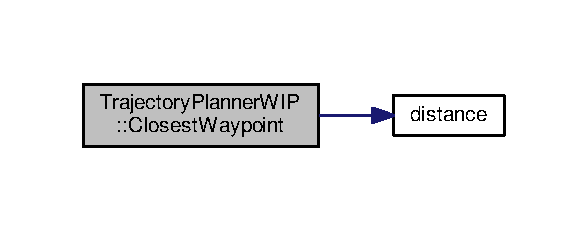
\includegraphics[width=282pt]{classTrajectoryPlannerWIP_a9f787291e9065422a9c649c6b24acf8e_cgraph}
\end{center}
\end{figure}


\index{Trajectory\+Planner\+W\+IP@{Trajectory\+Planner\+W\+IP}!get\+Frenet@{get\+Frenet}}
\index{get\+Frenet@{get\+Frenet}!Trajectory\+Planner\+W\+IP@{Trajectory\+Planner\+W\+IP}}
\subsubsection[{\texorpdfstring{get\+Frenet(double x, double y)}{getFrenet(double x, double y)}}]{\setlength{\rightskip}{0pt plus 5cm}vector$<$ double $>$ Trajectory\+Planner\+W\+I\+P\+::get\+Frenet (
\begin{DoxyParamCaption}
\item[{double}]{x, }
\item[{double}]{y}
\end{DoxyParamCaption}
)\hspace{0.3cm}{\ttfamily [protected]}}\hypertarget{classTrajectoryPlannerWIP_a90ba8175932f377a2f56795edb8eb1eb}{}\label{classTrajectoryPlannerWIP_a90ba8175932f377a2f56795edb8eb1eb}


Here is the call graph for this function\+:\nopagebreak
\begin{figure}[H]
\begin{center}
\leavevmode
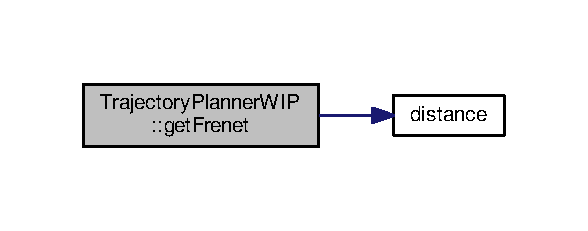
\includegraphics[width=282pt]{classTrajectoryPlannerWIP_a90ba8175932f377a2f56795edb8eb1eb_cgraph}
\end{center}
\end{figure}


\index{Trajectory\+Planner\+W\+IP@{Trajectory\+Planner\+W\+IP}!get\+Next\+Path\+Trajectory@{get\+Next\+Path\+Trajectory}}
\index{get\+Next\+Path\+Trajectory@{get\+Next\+Path\+Trajectory}!Trajectory\+Planner\+W\+IP@{Trajectory\+Planner\+W\+IP}}
\subsubsection[{\texorpdfstring{get\+Next\+Path\+Trajectory(double start\+\_\+s, double start\+\_\+d, double target\+\_\+lane, double current\+\_\+speed, double ref\+\_\+speed, double Time)}{getNextPathTrajectory(double start_s, double start_d, double target_lane, double current_speed, double ref_speed, double Time)}}]{\setlength{\rightskip}{0pt plus 5cm}vector$<$ vector$<$ double $>$ $>$ Trajectory\+Planner\+W\+I\+P\+::get\+Next\+Path\+Trajectory (
\begin{DoxyParamCaption}
\item[{double}]{start\+\_\+s, }
\item[{double}]{start\+\_\+d, }
\item[{double}]{target\+\_\+lane, }
\item[{double}]{current\+\_\+speed, }
\item[{double}]{ref\+\_\+speed, }
\item[{double}]{Time}
\end{DoxyParamCaption}
)}\hypertarget{classTrajectoryPlannerWIP_a9c53694540c32d1e724def363c20d310}{}\label{classTrajectoryPlannerWIP_a9c53694540c32d1e724def363c20d310}
\index{Trajectory\+Planner\+W\+IP@{Trajectory\+Planner\+W\+IP}!get\+XY@{get\+XY}}
\index{get\+XY@{get\+XY}!Trajectory\+Planner\+W\+IP@{Trajectory\+Planner\+W\+IP}}
\subsubsection[{\texorpdfstring{get\+X\+Y(double s, double d)}{getXY(double s, double d)}}]{\setlength{\rightskip}{0pt plus 5cm}vector$<$ double $>$ Trajectory\+Planner\+W\+I\+P\+::get\+XY (
\begin{DoxyParamCaption}
\item[{double}]{s, }
\item[{double}]{d}
\end{DoxyParamCaption}
)\hspace{0.3cm}{\ttfamily [protected]}}\hypertarget{classTrajectoryPlannerWIP_a6c4a03d5e4f4b78bdbd91debe2d1b246}{}\label{classTrajectoryPlannerWIP_a6c4a03d5e4f4b78bdbd91debe2d1b246}


Here is the call graph for this function\+:\nopagebreak
\begin{figure}[H]
\begin{center}
\leavevmode
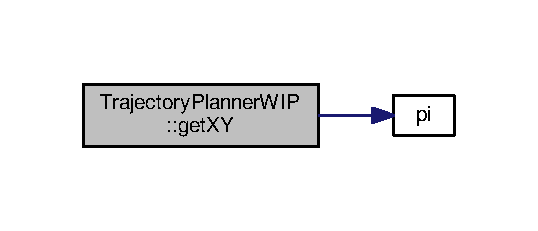
\includegraphics[width=258pt]{classTrajectoryPlannerWIP_a6c4a03d5e4f4b78bdbd91debe2d1b246_cgraph}
\end{center}
\end{figure}


\index{Trajectory\+Planner\+W\+IP@{Trajectory\+Planner\+W\+IP}!J\+MT@{J\+MT}}
\index{J\+MT@{J\+MT}!Trajectory\+Planner\+W\+IP@{Trajectory\+Planner\+W\+IP}}
\subsubsection[{\texorpdfstring{J\+M\+T(vector$<$ double $>$ start, vector$<$ double $>$ end, double T)}{JMT(vector< double > start, vector< double > end, double T)}}]{\setlength{\rightskip}{0pt plus 5cm}vector$<$ double $>$ Trajectory\+Planner\+W\+I\+P\+::\+J\+MT (
\begin{DoxyParamCaption}
\item[{vector$<$ double $>$}]{start, }
\item[{vector$<$ double $>$}]{end, }
\item[{double}]{T}
\end{DoxyParamCaption}
)\hspace{0.3cm}{\ttfamily [protected]}}\hypertarget{classTrajectoryPlannerWIP_ac2053a967111d1f776616ea7a473cfa0}{}\label{classTrajectoryPlannerWIP_ac2053a967111d1f776616ea7a473cfa0}
\index{Trajectory\+Planner\+W\+IP@{Trajectory\+Planner\+W\+IP}!load\+Map@{load\+Map}}
\index{load\+Map@{load\+Map}!Trajectory\+Planner\+W\+IP@{Trajectory\+Planner\+W\+IP}}
\subsubsection[{\texorpdfstring{load\+Map()}{loadMap()}}]{\setlength{\rightskip}{0pt plus 5cm}void Trajectory\+Planner\+W\+I\+P\+::load\+Map (
\begin{DoxyParamCaption}
{}
\end{DoxyParamCaption}
)}\hypertarget{classTrajectoryPlannerWIP_ae13818910d1d7b7a65eacf49ebd1682d}{}\label{classTrajectoryPlannerWIP_ae13818910d1d7b7a65eacf49ebd1682d}
\index{Trajectory\+Planner\+W\+IP@{Trajectory\+Planner\+W\+IP}!merge\+Trajectories@{merge\+Trajectories}}
\index{merge\+Trajectories@{merge\+Trajectories}!Trajectory\+Planner\+W\+IP@{Trajectory\+Planner\+W\+IP}}
\subsubsection[{\texorpdfstring{merge\+Trajectories(vector$<$ double $>$ previous\+\_\+path\+\_\+x, vector$<$ double $>$ previous\+\_\+path\+\_\+y, double end\+\_\+path\+\_\+s, double end\+\_\+path\+\_\+d, vector$<$ vector$<$ double $>$$>$ new\+Traj)}{mergeTrajectories(vector< double > previous_path_x, vector< double > previous_path_y, double end_path_s, double end_path_d, vector< vector< double >> newTraj)}}]{\setlength{\rightskip}{0pt plus 5cm}vector$<$ vector$<$ double $>$ $>$ Trajectory\+Planner\+W\+I\+P\+::merge\+Trajectories (
\begin{DoxyParamCaption}
\item[{vector$<$ double $>$}]{previous\+\_\+path\+\_\+x, }
\item[{vector$<$ double $>$}]{previous\+\_\+path\+\_\+y, }
\item[{double}]{end\+\_\+path\+\_\+s, }
\item[{double}]{end\+\_\+path\+\_\+d, }
\item[{vector$<$ vector$<$ double $>$$>$}]{new\+Traj}
\end{DoxyParamCaption}
)}\hypertarget{classTrajectoryPlannerWIP_aeb7dc782540b1e43b7be2f7075d23b75}{}\label{classTrajectoryPlannerWIP_aeb7dc782540b1e43b7be2f7075d23b75}
\index{Trajectory\+Planner\+W\+IP@{Trajectory\+Planner\+W\+IP}!Next\+Waypoint@{Next\+Waypoint}}
\index{Next\+Waypoint@{Next\+Waypoint}!Trajectory\+Planner\+W\+IP@{Trajectory\+Planner\+W\+IP}}
\subsubsection[{\texorpdfstring{Next\+Waypoint(double x, double y)}{NextWaypoint(double x, double y)}}]{\setlength{\rightskip}{0pt plus 5cm}int Trajectory\+Planner\+W\+I\+P\+::\+Next\+Waypoint (
\begin{DoxyParamCaption}
\item[{double}]{x, }
\item[{double}]{y}
\end{DoxyParamCaption}
)\hspace{0.3cm}{\ttfamily [protected]}}\hypertarget{classTrajectoryPlannerWIP_afcec4651796ba110751bddeb25f223fa}{}\label{classTrajectoryPlannerWIP_afcec4651796ba110751bddeb25f223fa}
\index{Trajectory\+Planner\+W\+IP@{Trajectory\+Planner\+W\+IP}!predict\+Next\+Endpoint@{predict\+Next\+Endpoint}}
\index{predict\+Next\+Endpoint@{predict\+Next\+Endpoint}!Trajectory\+Planner\+W\+IP@{Trajectory\+Planner\+W\+IP}}
\subsubsection[{\texorpdfstring{predict\+Next\+Endpoint(double start\+\_\+s, double start\+\_\+d, double lane, double current\+\_\+speed, double ref\+\_\+speed, double Time)}{predictNextEndpoint(double start_s, double start_d, double lane, double current_speed, double ref_speed, double Time)}}]{\setlength{\rightskip}{0pt plus 5cm}vector$<$ double $>$ Trajectory\+Planner\+W\+I\+P\+::predict\+Next\+Endpoint (
\begin{DoxyParamCaption}
\item[{double}]{start\+\_\+s, }
\item[{double}]{start\+\_\+d, }
\item[{double}]{lane, }
\item[{double}]{current\+\_\+speed, }
\item[{double}]{ref\+\_\+speed, }
\item[{double}]{Time}
\end{DoxyParamCaption}
)\hspace{0.3cm}{\ttfamily [protected]}}\hypertarget{classTrajectoryPlannerWIP_a836cd57fcddc08790c6c4a33249e3161}{}\label{classTrajectoryPlannerWIP_a836cd57fcddc08790c6c4a33249e3161}


\subsection{Member Data Documentation}
\index{Trajectory\+Planner\+W\+IP@{Trajectory\+Planner\+W\+IP}!end\+\_\+path\+\_\+d@{end\+\_\+path\+\_\+d}}
\index{end\+\_\+path\+\_\+d@{end\+\_\+path\+\_\+d}!Trajectory\+Planner\+W\+IP@{Trajectory\+Planner\+W\+IP}}
\subsubsection[{\texorpdfstring{end\+\_\+path\+\_\+d}{end_path_d}}]{\setlength{\rightskip}{0pt plus 5cm}double Trajectory\+Planner\+W\+I\+P\+::end\+\_\+path\+\_\+d}\hypertarget{classTrajectoryPlannerWIP_a45a0c4e41dae17e9387b358d472bdb55}{}\label{classTrajectoryPlannerWIP_a45a0c4e41dae17e9387b358d472bdb55}
\index{Trajectory\+Planner\+W\+IP@{Trajectory\+Planner\+W\+IP}!end\+\_\+path\+\_\+s@{end\+\_\+path\+\_\+s}}
\index{end\+\_\+path\+\_\+s@{end\+\_\+path\+\_\+s}!Trajectory\+Planner\+W\+IP@{Trajectory\+Planner\+W\+IP}}
\subsubsection[{\texorpdfstring{end\+\_\+path\+\_\+s}{end_path_s}}]{\setlength{\rightskip}{0pt plus 5cm}double Trajectory\+Planner\+W\+I\+P\+::end\+\_\+path\+\_\+s}\hypertarget{classTrajectoryPlannerWIP_a1239028b8c1d13c6e03237f160965112}{}\label{classTrajectoryPlannerWIP_a1239028b8c1d13c6e03237f160965112}
\index{Trajectory\+Planner\+W\+IP@{Trajectory\+Planner\+W\+IP}!map\+\_\+file\+\_\+@{map\+\_\+file\+\_\+}}
\index{map\+\_\+file\+\_\+@{map\+\_\+file\+\_\+}!Trajectory\+Planner\+W\+IP@{Trajectory\+Planner\+W\+IP}}
\subsubsection[{\texorpdfstring{map\+\_\+file\+\_\+}{map_file_}}]{\setlength{\rightskip}{0pt plus 5cm}string Trajectory\+Planner\+W\+I\+P\+::map\+\_\+file\+\_\+ = \char`\"{}../data/highway\+\_\+map.\+csv\char`\"{}\hspace{0.3cm}{\ttfamily [protected]}}\hypertarget{classTrajectoryPlannerWIP_a87aa1ae8bce8788c8fab3db76b92997c}{}\label{classTrajectoryPlannerWIP_a87aa1ae8bce8788c8fab3db76b92997c}
\index{Trajectory\+Planner\+W\+IP@{Trajectory\+Planner\+W\+IP}!maps\+\_\+dx@{maps\+\_\+dx}}
\index{maps\+\_\+dx@{maps\+\_\+dx}!Trajectory\+Planner\+W\+IP@{Trajectory\+Planner\+W\+IP}}
\subsubsection[{\texorpdfstring{maps\+\_\+dx}{maps_dx}}]{\setlength{\rightskip}{0pt plus 5cm}vector$<$double$>$ Trajectory\+Planner\+W\+I\+P\+::maps\+\_\+dx\hspace{0.3cm}{\ttfamily [protected]}}\hypertarget{classTrajectoryPlannerWIP_a60657fd8df138c58a1a9333f07f73f7e}{}\label{classTrajectoryPlannerWIP_a60657fd8df138c58a1a9333f07f73f7e}
\index{Trajectory\+Planner\+W\+IP@{Trajectory\+Planner\+W\+IP}!maps\+\_\+dy@{maps\+\_\+dy}}
\index{maps\+\_\+dy@{maps\+\_\+dy}!Trajectory\+Planner\+W\+IP@{Trajectory\+Planner\+W\+IP}}
\subsubsection[{\texorpdfstring{maps\+\_\+dy}{maps_dy}}]{\setlength{\rightskip}{0pt plus 5cm}vector$<$double$>$ Trajectory\+Planner\+W\+I\+P\+::maps\+\_\+dy\hspace{0.3cm}{\ttfamily [protected]}}\hypertarget{classTrajectoryPlannerWIP_ae1fd51251d18023cc395eff388785b13}{}\label{classTrajectoryPlannerWIP_ae1fd51251d18023cc395eff388785b13}
\index{Trajectory\+Planner\+W\+IP@{Trajectory\+Planner\+W\+IP}!maps\+\_\+s@{maps\+\_\+s}}
\index{maps\+\_\+s@{maps\+\_\+s}!Trajectory\+Planner\+W\+IP@{Trajectory\+Planner\+W\+IP}}
\subsubsection[{\texorpdfstring{maps\+\_\+s}{maps_s}}]{\setlength{\rightskip}{0pt plus 5cm}vector$<$double$>$ Trajectory\+Planner\+W\+I\+P\+::maps\+\_\+s\hspace{0.3cm}{\ttfamily [protected]}}\hypertarget{classTrajectoryPlannerWIP_a38af64be0ca058c3ac72d6cf2883de9f}{}\label{classTrajectoryPlannerWIP_a38af64be0ca058c3ac72d6cf2883de9f}
\index{Trajectory\+Planner\+W\+IP@{Trajectory\+Planner\+W\+IP}!maps\+\_\+x@{maps\+\_\+x}}
\index{maps\+\_\+x@{maps\+\_\+x}!Trajectory\+Planner\+W\+IP@{Trajectory\+Planner\+W\+IP}}
\subsubsection[{\texorpdfstring{maps\+\_\+x}{maps_x}}]{\setlength{\rightskip}{0pt plus 5cm}vector$<$double$>$ Trajectory\+Planner\+W\+I\+P\+::maps\+\_\+x\hspace{0.3cm}{\ttfamily [protected]}}\hypertarget{classTrajectoryPlannerWIP_abaa6f54058eb01c7c16df360c6883496}{}\label{classTrajectoryPlannerWIP_abaa6f54058eb01c7c16df360c6883496}
\index{Trajectory\+Planner\+W\+IP@{Trajectory\+Planner\+W\+IP}!maps\+\_\+y@{maps\+\_\+y}}
\index{maps\+\_\+y@{maps\+\_\+y}!Trajectory\+Planner\+W\+IP@{Trajectory\+Planner\+W\+IP}}
\subsubsection[{\texorpdfstring{maps\+\_\+y}{maps_y}}]{\setlength{\rightskip}{0pt plus 5cm}vector$<$double$>$ Trajectory\+Planner\+W\+I\+P\+::maps\+\_\+y\hspace{0.3cm}{\ttfamily [protected]}}\hypertarget{classTrajectoryPlannerWIP_a17cfcc4b66e5fff8a1802e5fc9dd7639}{}\label{classTrajectoryPlannerWIP_a17cfcc4b66e5fff8a1802e5fc9dd7639}
\index{Trajectory\+Planner\+W\+IP@{Trajectory\+Planner\+W\+IP}!max\+\_\+s@{max\+\_\+s}}
\index{max\+\_\+s@{max\+\_\+s}!Trajectory\+Planner\+W\+IP@{Trajectory\+Planner\+W\+IP}}
\subsubsection[{\texorpdfstring{max\+\_\+s}{max_s}}]{\setlength{\rightskip}{0pt plus 5cm}double Trajectory\+Planner\+W\+I\+P\+::max\+\_\+s = 6945.\+554\hspace{0.3cm}{\ttfamily [protected]}}\hypertarget{classTrajectoryPlannerWIP_a43501cae77daf85f811ed0873d9bf960}{}\label{classTrajectoryPlannerWIP_a43501cae77daf85f811ed0873d9bf960}
\index{Trajectory\+Planner\+W\+IP@{Trajectory\+Planner\+W\+IP}!previous\+\_\+path\+\_\+x@{previous\+\_\+path\+\_\+x}}
\index{previous\+\_\+path\+\_\+x@{previous\+\_\+path\+\_\+x}!Trajectory\+Planner\+W\+IP@{Trajectory\+Planner\+W\+IP}}
\subsubsection[{\texorpdfstring{previous\+\_\+path\+\_\+x}{previous_path_x}}]{\setlength{\rightskip}{0pt plus 5cm}vector$<$double$>$ Trajectory\+Planner\+W\+I\+P\+::previous\+\_\+path\+\_\+x}\hypertarget{classTrajectoryPlannerWIP_a74997cfa081e6d4409d4d2234e5b3855}{}\label{classTrajectoryPlannerWIP_a74997cfa081e6d4409d4d2234e5b3855}
\index{Trajectory\+Planner\+W\+IP@{Trajectory\+Planner\+W\+IP}!previous\+\_\+path\+\_\+y@{previous\+\_\+path\+\_\+y}}
\index{previous\+\_\+path\+\_\+y@{previous\+\_\+path\+\_\+y}!Trajectory\+Planner\+W\+IP@{Trajectory\+Planner\+W\+IP}}
\subsubsection[{\texorpdfstring{previous\+\_\+path\+\_\+y}{previous_path_y}}]{\setlength{\rightskip}{0pt plus 5cm}vector$<$double$>$ Trajectory\+Planner\+W\+I\+P\+::previous\+\_\+path\+\_\+y}\hypertarget{classTrajectoryPlannerWIP_a32a8ed201b7abf6a5817e17ba5e4fca3}{}\label{classTrajectoryPlannerWIP_a32a8ed201b7abf6a5817e17ba5e4fca3}


The documentation for this class was generated from the following files\+:\begin{DoxyCompactItemize}
\item 
src/\hyperlink{TrajectoryPlannerWIP_8h}{Trajectory\+Planner\+W\+I\+P.\+h}\item 
src/\hyperlink{TrajectoryPlannerWIP_8cpp}{Trajectory\+Planner\+W\+I\+P.\+cpp}\end{DoxyCompactItemize}

\chapter{File Documentation}
\hypertarget{AbstractVehicle_8cpp}{}\section{src/\+Abstract\+Vehicle.cpp File Reference}
\label{AbstractVehicle_8cpp}\index{src/\+Abstract\+Vehicle.\+cpp@{src/\+Abstract\+Vehicle.\+cpp}}
{\ttfamily \#include \char`\"{}helper.\+h\char`\"{}}\\*
{\ttfamily \#include $<$algorithm$>$}\\*
{\ttfamily \#include $<$math.\+h$>$}\\*
{\ttfamily \#include $<$vector$>$}\\*
{\ttfamily \#include \char`\"{}Ego\+Vehicle.\+h\char`\"{}}\\*
Include dependency graph for Abstract\+Vehicle.\+cpp\+:\nopagebreak
\begin{figure}[H]
\begin{center}
\leavevmode
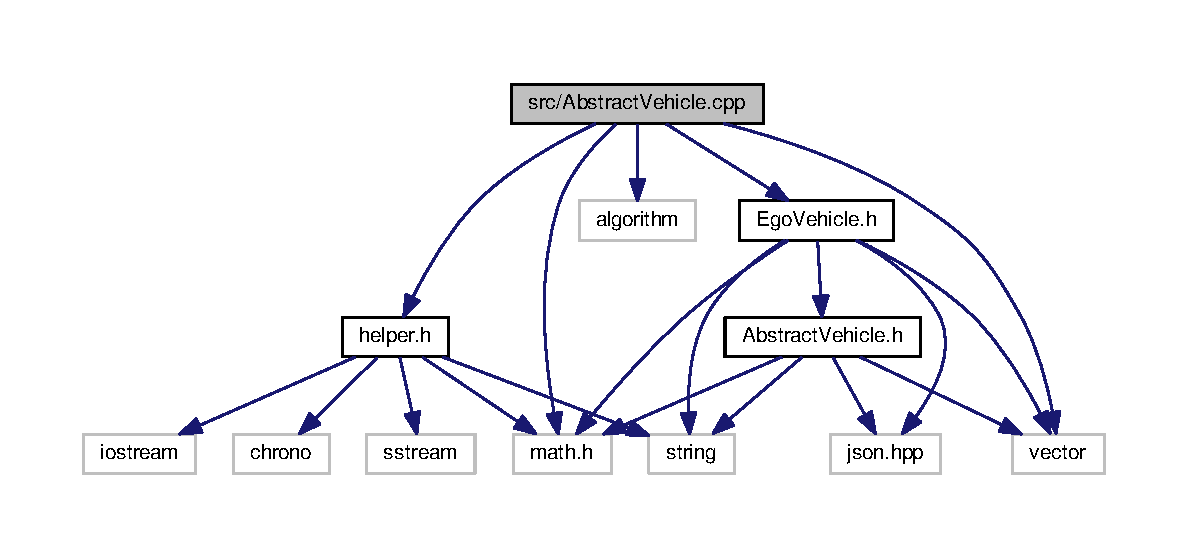
\includegraphics[width=350pt]{AbstractVehicle_8cpp__incl}
\end{center}
\end{figure}

\hypertarget{AbstractVehicle_8h}{}\section{src/\+Abstract\+Vehicle.h File Reference}
\label{AbstractVehicle_8h}\index{src/\+Abstract\+Vehicle.\+h@{src/\+Abstract\+Vehicle.\+h}}
{\ttfamily \#include $<$math.\+h$>$}\\*
{\ttfamily \#include $<$string$>$}\\*
{\ttfamily \#include $<$vector$>$}\\*
{\ttfamily \#include \char`\"{}json.\+hpp\char`\"{}}\\*
Include dependency graph for Abstract\+Vehicle.\+h\+:\nopagebreak
\begin{figure}[H]
\begin{center}
\leavevmode
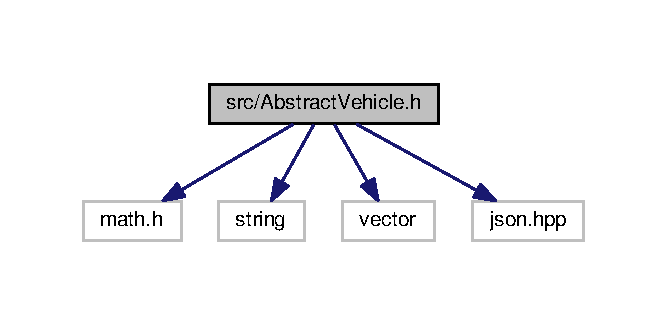
\includegraphics[width=320pt]{AbstractVehicle_8h__incl}
\end{center}
\end{figure}
This graph shows which files directly or indirectly include this file\+:\nopagebreak
\begin{figure}[H]
\begin{center}
\leavevmode
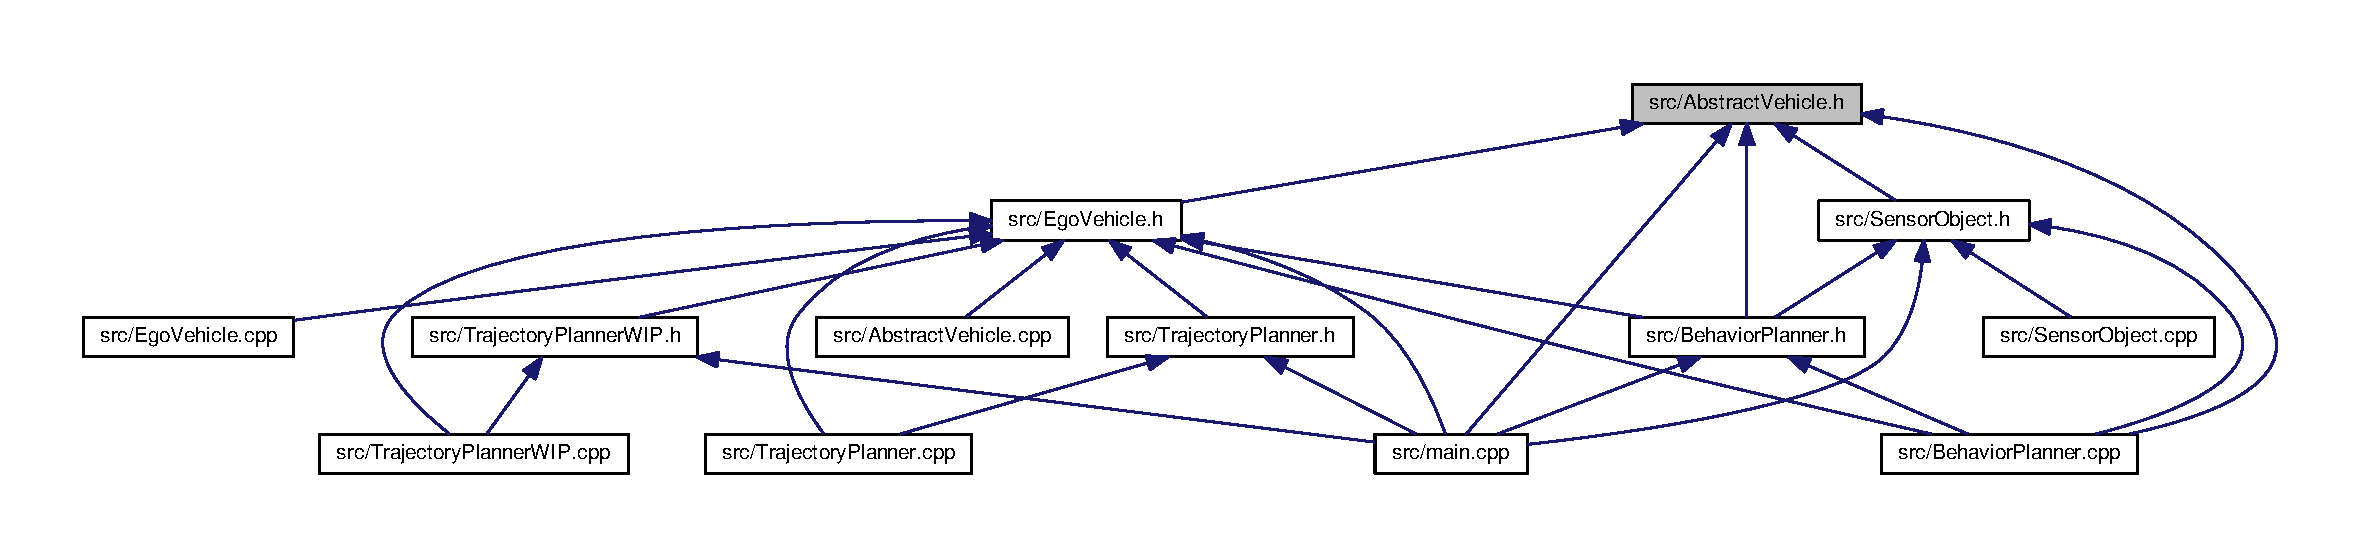
\includegraphics[width=350pt]{AbstractVehicle_8h__dep__incl}
\end{center}
\end{figure}
\subsection*{Classes}
\begin{DoxyCompactItemize}
\item 
class \hyperlink{classAbstractVehicle}{Abstract\+Vehicle}
\end{DoxyCompactItemize}

\hypertarget{BehaviorPlanner_8cpp}{}\section{src/\+Behavior\+Planner.cpp File Reference}
\label{BehaviorPlanner_8cpp}\index{src/\+Behavior\+Planner.\+cpp@{src/\+Behavior\+Planner.\+cpp}}
{\ttfamily \#include \char`\"{}Abstract\+Vehicle.\+h\char`\"{}}\\*
{\ttfamily \#include \char`\"{}Ego\+Vehicle.\+h\char`\"{}}\\*
{\ttfamily \#include \char`\"{}Sensor\+Object.\+h\char`\"{}}\\*
{\ttfamily \#include \char`\"{}Behavior\+Planner.\+h\char`\"{}}\\*
{\ttfamily \#include $<$set$>$}\\*
Include dependency graph for Behavior\+Planner.\+cpp\+:\nopagebreak
\begin{figure}[H]
\begin{center}
\leavevmode
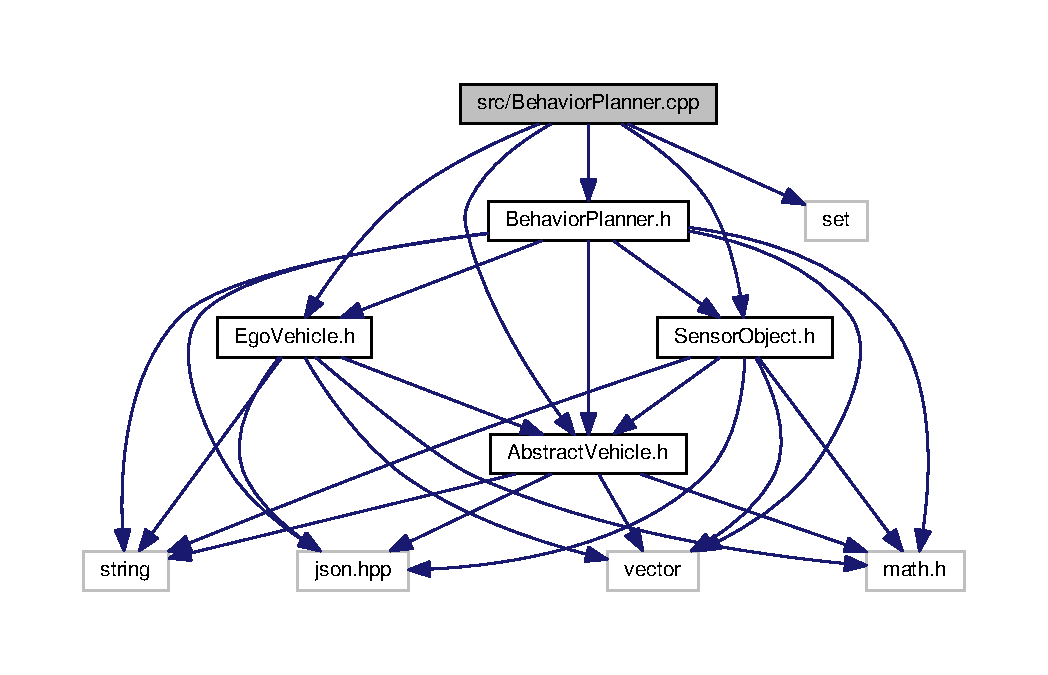
\includegraphics[width=350pt]{BehaviorPlanner_8cpp__incl}
\end{center}
\end{figure}

\hypertarget{BehaviorPlanner_8h}{}\section{src/\+Behavior\+Planner.h File Reference}
\label{BehaviorPlanner_8h}\index{src/\+Behavior\+Planner.\+h@{src/\+Behavior\+Planner.\+h}}
{\ttfamily \#include \char`\"{}json.\+hpp\char`\"{}}\\*
{\ttfamily \#include $<$math.\+h$>$}\\*
{\ttfamily \#include $<$vector$>$}\\*
{\ttfamily \#include \char`\"{}Abstract\+Vehicle.\+h\char`\"{}}\\*
{\ttfamily \#include \char`\"{}Ego\+Vehicle.\+h\char`\"{}}\\*
{\ttfamily \#include \char`\"{}Sensor\+Object.\+h\char`\"{}}\\*
{\ttfamily \#include $<$string$>$}\\*
Include dependency graph for Behavior\+Planner.\+h\+:\nopagebreak
\begin{figure}[H]
\begin{center}
\leavevmode
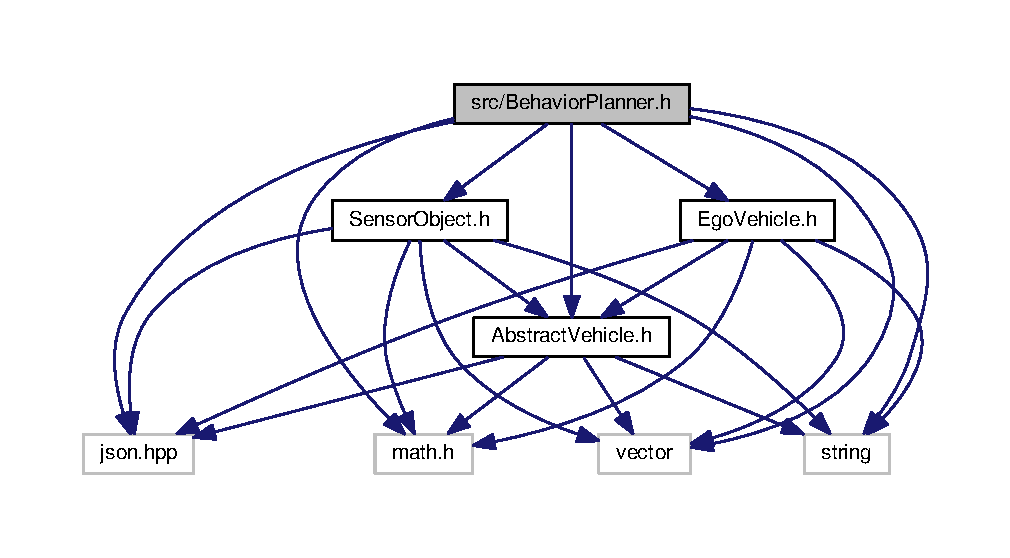
\includegraphics[width=350pt]{BehaviorPlanner_8h__incl}
\end{center}
\end{figure}
This graph shows which files directly or indirectly include this file\+:\nopagebreak
\begin{figure}[H]
\begin{center}
\leavevmode
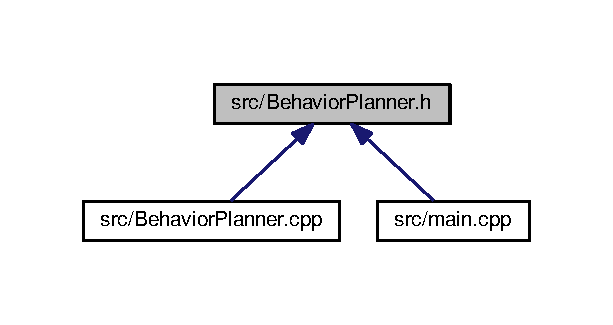
\includegraphics[width=294pt]{BehaviorPlanner_8h__dep__incl}
\end{center}
\end{figure}
\subsection*{Classes}
\begin{DoxyCompactItemize}
\item 
class \hyperlink{classBehaviorPlanner}{Behavior\+Planner}
\end{DoxyCompactItemize}

\hypertarget{EgoVehicle_8cpp}{}\section{src/\+Ego\+Vehicle.cpp File Reference}
\label{EgoVehicle_8cpp}\index{src/\+Ego\+Vehicle.\+cpp@{src/\+Ego\+Vehicle.\+cpp}}
{\ttfamily \#include \char`\"{}helper.\+h\char`\"{}}\\*
{\ttfamily \#include $<$algorithm$>$}\\*
{\ttfamily \#include $<$math.\+h$>$}\\*
{\ttfamily \#include $<$vector$>$}\\*
{\ttfamily \#include \char`\"{}Ego\+Vehicle.\+h\char`\"{}}\\*
Include dependency graph for Ego\+Vehicle.\+cpp\+:\nopagebreak
\begin{figure}[H]
\begin{center}
\leavevmode
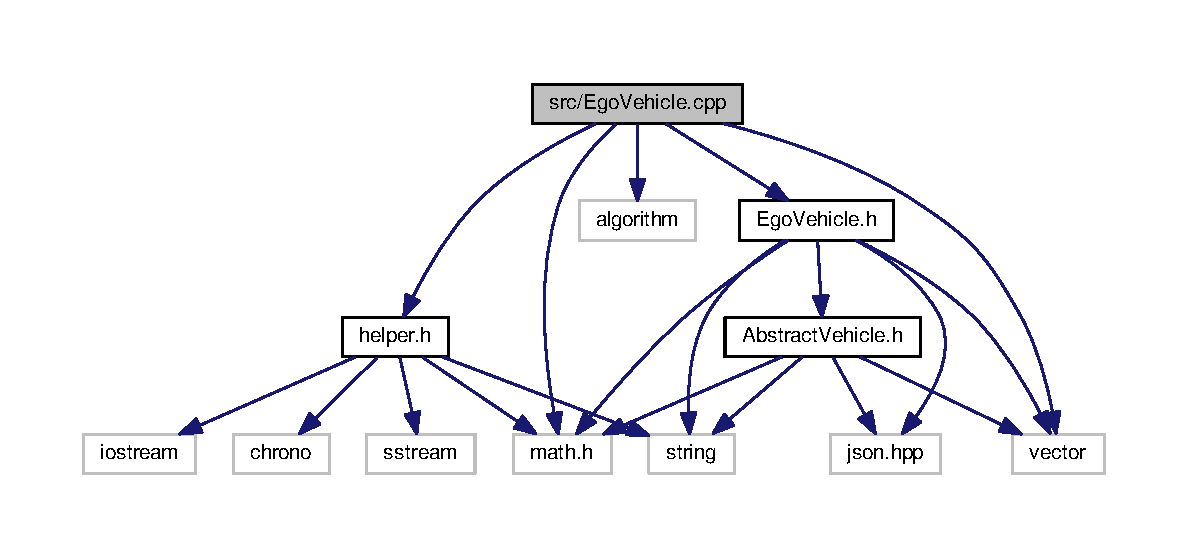
\includegraphics[width=350pt]{EgoVehicle_8cpp__incl}
\end{center}
\end{figure}

\hypertarget{EgoVehicle_8h}{}\section{src/\+Ego\+Vehicle.h File Reference}
\label{EgoVehicle_8h}\index{src/\+Ego\+Vehicle.\+h@{src/\+Ego\+Vehicle.\+h}}
{\ttfamily \#include \char`\"{}json.\+hpp\char`\"{}}\\*
{\ttfamily \#include $<$math.\+h$>$}\\*
{\ttfamily \#include $<$vector$>$}\\*
{\ttfamily \#include \char`\"{}Abstract\+Vehicle.\+h\char`\"{}}\\*
{\ttfamily \#include $<$string$>$}\\*
Include dependency graph for Ego\+Vehicle.\+h\+:\nopagebreak
\begin{figure}[H]
\begin{center}
\leavevmode
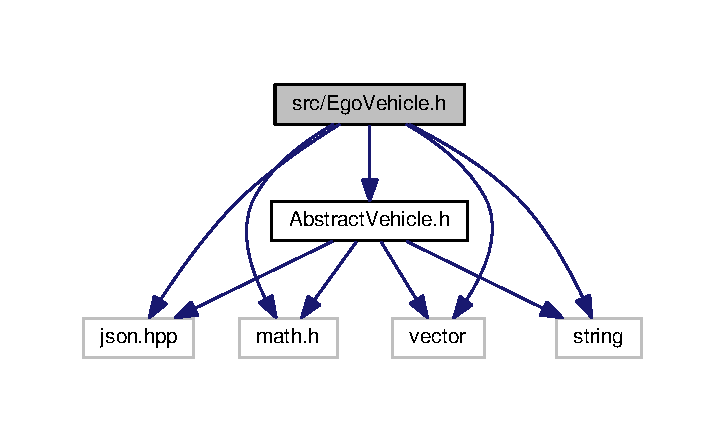
\includegraphics[width=348pt]{EgoVehicle_8h__incl}
\end{center}
\end{figure}
This graph shows which files directly or indirectly include this file\+:\nopagebreak
\begin{figure}[H]
\begin{center}
\leavevmode
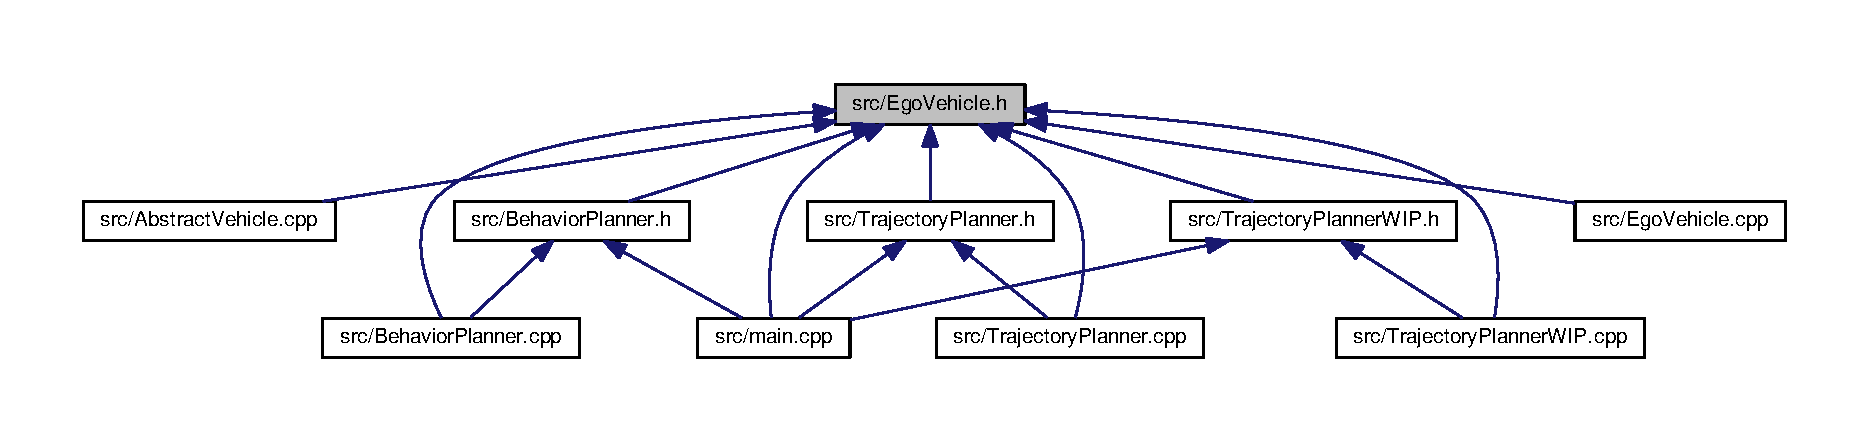
\includegraphics[width=350pt]{EgoVehicle_8h__dep__incl}
\end{center}
\end{figure}
\subsection*{Classes}
\begin{DoxyCompactItemize}
\item 
class \hyperlink{classEgoVehicle}{Ego\+Vehicle}
\end{DoxyCompactItemize}

\hypertarget{helper_8h}{}\section{src/helper.h File Reference}
\label{helper_8h}\index{src/helper.\+h@{src/helper.\+h}}
{\ttfamily \#include $<$string$>$}\\*
{\ttfamily \#include $<$sstream$>$}\\*
{\ttfamily \#include $<$iostream$>$}\\*
{\ttfamily \#include $<$chrono$>$}\\*
{\ttfamily \#include $<$math.\+h$>$}\\*
Include dependency graph for helper.\+h\+:\nopagebreak
\begin{figure}[H]
\begin{center}
\leavevmode
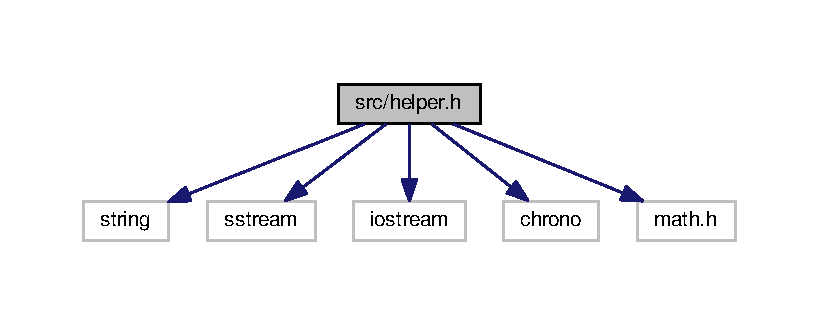
\includegraphics[width=350pt]{helper_8h__incl}
\end{center}
\end{figure}
This graph shows which files directly or indirectly include this file\+:\nopagebreak
\begin{figure}[H]
\begin{center}
\leavevmode
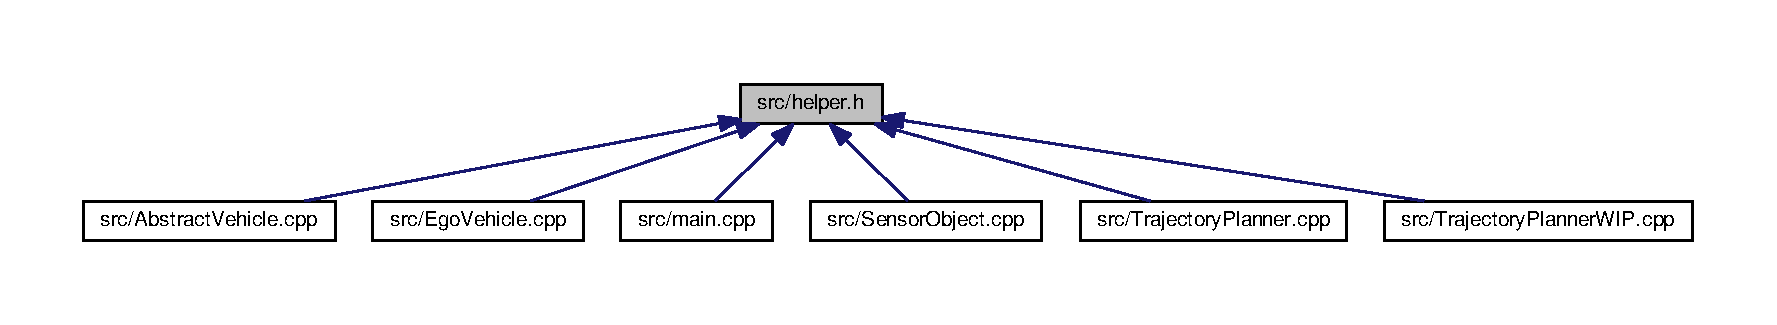
\includegraphics[width=350pt]{helper_8h__dep__incl}
\end{center}
\end{figure}
\subsection*{Classes}
\begin{DoxyCompactItemize}
\item 
class \hyperlink{classTimer}{Timer}
\end{DoxyCompactItemize}
\subsection*{Functions}
\begin{DoxyCompactItemize}
\item 
{\footnotesize template$<$typename T $>$ }\\std\+::string \hyperlink{helper_8h_a9d8f0fd0cc93af82fed5b259bb45c679}{to\+\_\+string} (T const \&value)
\end{DoxyCompactItemize}


\subsection{Function Documentation}
\index{helper.\+h@{helper.\+h}!to\+\_\+string@{to\+\_\+string}}
\index{to\+\_\+string@{to\+\_\+string}!helper.\+h@{helper.\+h}}
\subsubsection[{\texorpdfstring{to\+\_\+string(\+T const \&value)}{to_string(T const &value)}}]{\setlength{\rightskip}{0pt plus 5cm}template$<$typename T $>$ std\+::string to\+\_\+string (
\begin{DoxyParamCaption}
\item[{T const \&}]{value}
\end{DoxyParamCaption}
)}\hypertarget{helper_8h_a9d8f0fd0cc93af82fed5b259bb45c679}{}\label{helper_8h_a9d8f0fd0cc93af82fed5b259bb45c679}

\hypertarget{main_8cpp}{}\section{src/main.cpp File Reference}
\label{main_8cpp}\index{src/main.\+cpp@{src/main.\+cpp}}
{\ttfamily \#include \char`\"{}Eigen-\/3.\+3/\+Eigen/\+Core\char`\"{}}\\*
{\ttfamily \#include \char`\"{}Eigen-\/3.\+3/\+Eigen/\+QR\char`\"{}}\\*
{\ttfamily \#include \char`\"{}json.\+hpp\char`\"{}}\\*
{\ttfamily \#include \char`\"{}spline.\+h\char`\"{}}\\*
{\ttfamily \#include $<$chrono$>$}\\*
{\ttfamily \#include $<$fstream$>$}\\*
{\ttfamily \#include $<$iostream$>$}\\*
{\ttfamily \#include $<$math.\+h$>$}\\*
{\ttfamily \#include $<$thread$>$}\\*
{\ttfamily \#include $<$u\+W\+S/u\+W\+S.\+h$>$}\\*
{\ttfamily \#include $<$vector$>$}\\*
{\ttfamily \#include \char`\"{}Abstract\+Vehicle.\+h\char`\"{}}\\*
{\ttfamily \#include \char`\"{}Ego\+Vehicle.\+h\char`\"{}}\\*
{\ttfamily \#include \char`\"{}Sensor\+Object.\+h\char`\"{}}\\*
{\ttfamily \#include \char`\"{}Behavior\+Planner.\+h\char`\"{}}\\*
{\ttfamily \#include \char`\"{}Trajectory\+Planner.\+h\char`\"{}}\\*
{\ttfamily \#include \char`\"{}Trajectory\+Planner\+W\+I\+P.\+h\char`\"{}}\\*
{\ttfamily \#include \char`\"{}helper.\+h\char`\"{}}\\*
\subsection*{Typedefs}
\begin{DoxyCompactItemize}
\item 
using \hyperlink{main_8cpp_ab701e3ac61a85b337ec5c1abaad6742d}{json} = nlohmann\+::json
\end{DoxyCompactItemize}
\subsection*{Functions}
\begin{DoxyCompactItemize}
\item 
double \hyperlink{main_8cpp_a7d653a23bc3022afd9b32e419abbbc2d}{distance} (double x1, double y1, double x2, double y2)
\item 
double \hyperlink{main_8cpp_a19481c763d7a0b56b40eade0a21daab7}{pi} ()
\item 
double \hyperlink{main_8cpp_adbcf4609758c05a6405c3d9c5f185e6b}{deg2rad} (double x)
\item 
double \hyperlink{main_8cpp_aed6ee8bde39415298883a363b7759381}{rad2deg} (double x)
\item 
string \hyperlink{main_8cpp_a5d865119e9416cc7964648f6461f428e}{has\+Data} (string s)
\item 
int \hyperlink{main_8cpp_ae66f6b31b5ad750f1fe042a706a4e3d4}{main} ()
\end{DoxyCompactItemize}
\subsection*{Variables}
\begin{DoxyCompactItemize}
\item 
vector$<$ string $>$ \hyperlink{main_8cpp_a4db73d1b51ddd9bb512800cb1dc02285}{man\+\_\+str} \{\char`\"{}do nothing\char`\"{},\char`\"{}acc\char`\"{} ,\char`\"{}decc\char`\"{} ,\char`\"{}left\char`\"{},\char`\"{}right\char`\"{}\}
\end{DoxyCompactItemize}


\subsection{Typedef Documentation}
\index{main.\+cpp@{main.\+cpp}!json@{json}}
\index{json@{json}!main.\+cpp@{main.\+cpp}}
\subsubsection[{\texorpdfstring{json}{json}}]{\setlength{\rightskip}{0pt plus 5cm}using {\bf json} =  nlohmann\+::json}\hypertarget{main_8cpp_ab701e3ac61a85b337ec5c1abaad6742d}{}\label{main_8cpp_ab701e3ac61a85b337ec5c1abaad6742d}


\subsection{Function Documentation}
\index{main.\+cpp@{main.\+cpp}!deg2rad@{deg2rad}}
\index{deg2rad@{deg2rad}!main.\+cpp@{main.\+cpp}}
\subsubsection[{\texorpdfstring{deg2rad(double x)}{deg2rad(double x)}}]{\setlength{\rightskip}{0pt plus 5cm}double deg2rad (
\begin{DoxyParamCaption}
\item[{double}]{x}
\end{DoxyParamCaption}
)}\hypertarget{main_8cpp_adbcf4609758c05a6405c3d9c5f185e6b}{}\label{main_8cpp_adbcf4609758c05a6405c3d9c5f185e6b}


Here is the call graph for this function\+:\nopagebreak
\begin{figure}[H]
\begin{center}
\leavevmode
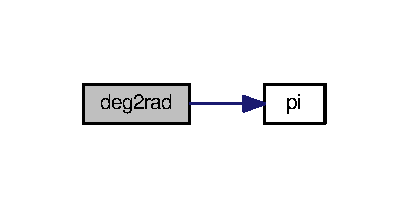
\includegraphics[width=196pt]{main_8cpp_adbcf4609758c05a6405c3d9c5f185e6b_cgraph}
\end{center}
\end{figure}


\index{main.\+cpp@{main.\+cpp}!distance@{distance}}
\index{distance@{distance}!main.\+cpp@{main.\+cpp}}
\subsubsection[{\texorpdfstring{distance(double x1, double y1, double x2, double y2)}{distance(double x1, double y1, double x2, double y2)}}]{\setlength{\rightskip}{0pt plus 5cm}double distance (
\begin{DoxyParamCaption}
\item[{double}]{x1, }
\item[{double}]{y1, }
\item[{double}]{x2, }
\item[{double}]{y2}
\end{DoxyParamCaption}
)}\hypertarget{main_8cpp_a7d653a23bc3022afd9b32e419abbbc2d}{}\label{main_8cpp_a7d653a23bc3022afd9b32e419abbbc2d}
\index{main.\+cpp@{main.\+cpp}!has\+Data@{has\+Data}}
\index{has\+Data@{has\+Data}!main.\+cpp@{main.\+cpp}}
\subsubsection[{\texorpdfstring{has\+Data(string s)}{hasData(string s)}}]{\setlength{\rightskip}{0pt plus 5cm}string has\+Data (
\begin{DoxyParamCaption}
\item[{string}]{s}
\end{DoxyParamCaption}
)}\hypertarget{main_8cpp_a5d865119e9416cc7964648f6461f428e}{}\label{main_8cpp_a5d865119e9416cc7964648f6461f428e}
\index{main.\+cpp@{main.\+cpp}!main@{main}}
\index{main@{main}!main.\+cpp@{main.\+cpp}}
\subsubsection[{\texorpdfstring{main()}{main()}}]{\setlength{\rightskip}{0pt plus 5cm}int main (
\begin{DoxyParamCaption}
{}
\end{DoxyParamCaption}
)}\hypertarget{main_8cpp_ae66f6b31b5ad750f1fe042a706a4e3d4}{}\label{main_8cpp_ae66f6b31b5ad750f1fe042a706a4e3d4}


Here is the call graph for this function\+:\nopagebreak
\begin{figure}[H]
\begin{center}
\leavevmode
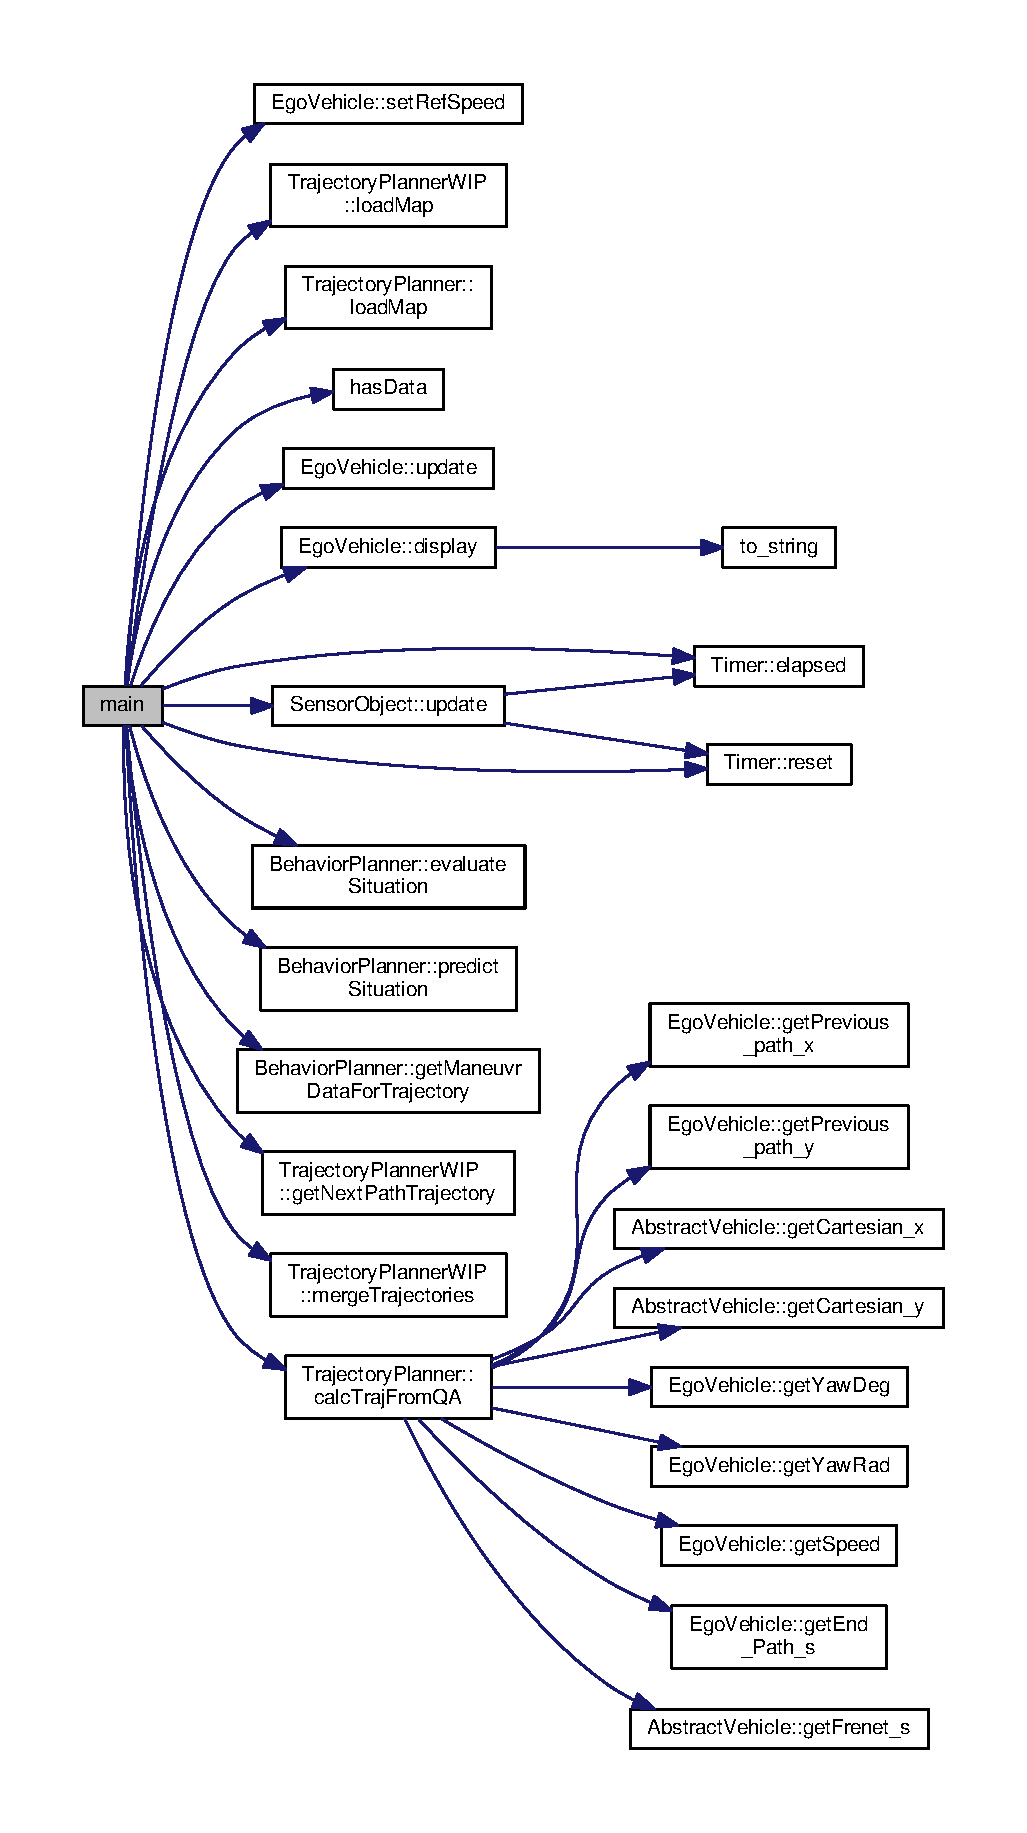
\includegraphics[height=550pt]{main_8cpp_ae66f6b31b5ad750f1fe042a706a4e3d4_cgraph}
\end{center}
\end{figure}


\index{main.\+cpp@{main.\+cpp}!pi@{pi}}
\index{pi@{pi}!main.\+cpp@{main.\+cpp}}
\subsubsection[{\texorpdfstring{pi()}{pi()}}]{\setlength{\rightskip}{0pt plus 5cm}double pi (
\begin{DoxyParamCaption}
{}
\end{DoxyParamCaption}
)}\hypertarget{main_8cpp_a19481c763d7a0b56b40eade0a21daab7}{}\label{main_8cpp_a19481c763d7a0b56b40eade0a21daab7}
\index{main.\+cpp@{main.\+cpp}!rad2deg@{rad2deg}}
\index{rad2deg@{rad2deg}!main.\+cpp@{main.\+cpp}}
\subsubsection[{\texorpdfstring{rad2deg(double x)}{rad2deg(double x)}}]{\setlength{\rightskip}{0pt plus 5cm}double rad2deg (
\begin{DoxyParamCaption}
\item[{double}]{x}
\end{DoxyParamCaption}
)}\hypertarget{main_8cpp_aed6ee8bde39415298883a363b7759381}{}\label{main_8cpp_aed6ee8bde39415298883a363b7759381}


Here is the call graph for this function\+:\nopagebreak
\begin{figure}[H]
\begin{center}
\leavevmode
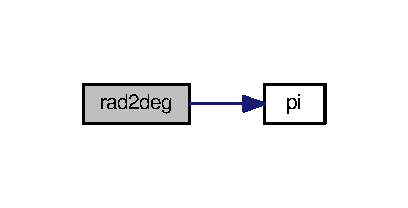
\includegraphics[width=196pt]{main_8cpp_aed6ee8bde39415298883a363b7759381_cgraph}
\end{center}
\end{figure}




\subsection{Variable Documentation}
\index{main.\+cpp@{main.\+cpp}!man\+\_\+str@{man\+\_\+str}}
\index{man\+\_\+str@{man\+\_\+str}!main.\+cpp@{main.\+cpp}}
\subsubsection[{\texorpdfstring{man\+\_\+str}{man_str}}]{\setlength{\rightskip}{0pt plus 5cm}vector$<$string$>$ man\+\_\+str \{\char`\"{}do nothing\char`\"{},\char`\"{}acc\char`\"{} ,\char`\"{}decc\char`\"{} ,\char`\"{}left\char`\"{},\char`\"{}right\char`\"{}\}}\hypertarget{main_8cpp_a4db73d1b51ddd9bb512800cb1dc02285}{}\label{main_8cpp_a4db73d1b51ddd9bb512800cb1dc02285}

\hypertarget{SensorObject_8cpp}{}\section{src/\+Sensor\+Object.cpp File Reference}
\label{SensorObject_8cpp}\index{src/\+Sensor\+Object.\+cpp@{src/\+Sensor\+Object.\+cpp}}
{\ttfamily \#include \char`\"{}helper.\+h\char`\"{}}\\*
{\ttfamily \#include $<$algorithm$>$}\\*
{\ttfamily \#include $<$math.\+h$>$}\\*
{\ttfamily \#include $<$vector$>$}\\*
{\ttfamily \#include \char`\"{}Sensor\+Object.\+h\char`\"{}}\\*
Include dependency graph for Sensor\+Object.\+cpp\+:\nopagebreak
\begin{figure}[H]
\begin{center}
\leavevmode
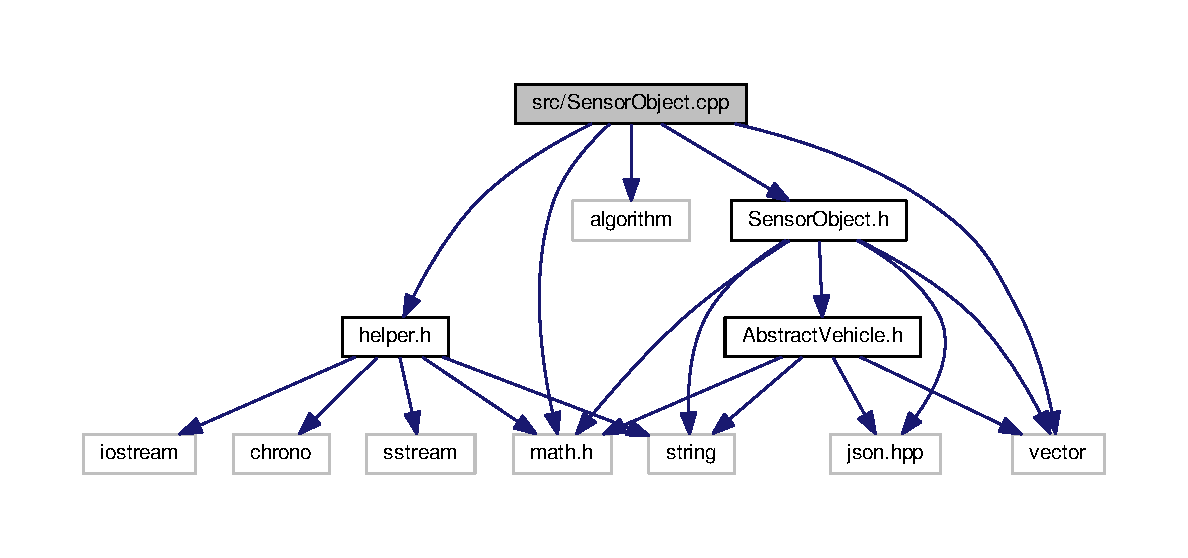
\includegraphics[width=350pt]{SensorObject_8cpp__incl}
\end{center}
\end{figure}

\hypertarget{SensorObject_8h}{}\section{src/\+Sensor\+Object.h File Reference}
\label{SensorObject_8h}\index{src/\+Sensor\+Object.\+h@{src/\+Sensor\+Object.\+h}}
{\ttfamily \#include \char`\"{}Abstract\+Vehicle.\+h\char`\"{}}\\*
{\ttfamily \#include \char`\"{}json.\+hpp\char`\"{}}\\*
{\ttfamily \#include $<$math.\+h$>$}\\*
{\ttfamily \#include $<$string$>$}\\*
{\ttfamily \#include $<$vector$>$}\\*
Include dependency graph for Sensor\+Object.\+h\+:\nopagebreak
\begin{figure}[H]
\begin{center}
\leavevmode
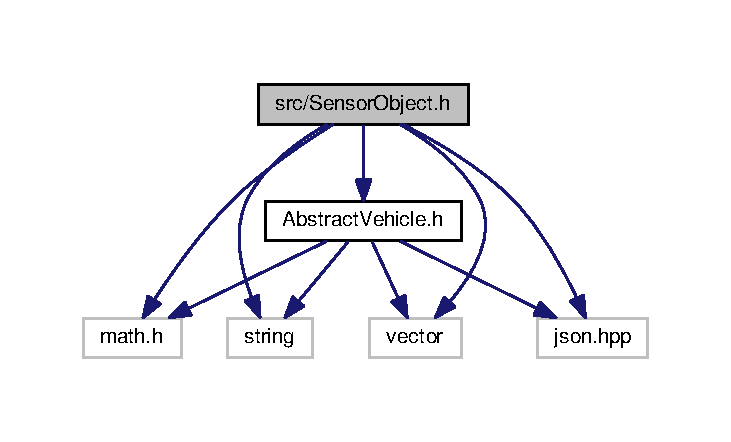
\includegraphics[width=350pt]{SensorObject_8h__incl}
\end{center}
\end{figure}
This graph shows which files directly or indirectly include this file\+:\nopagebreak
\begin{figure}[H]
\begin{center}
\leavevmode
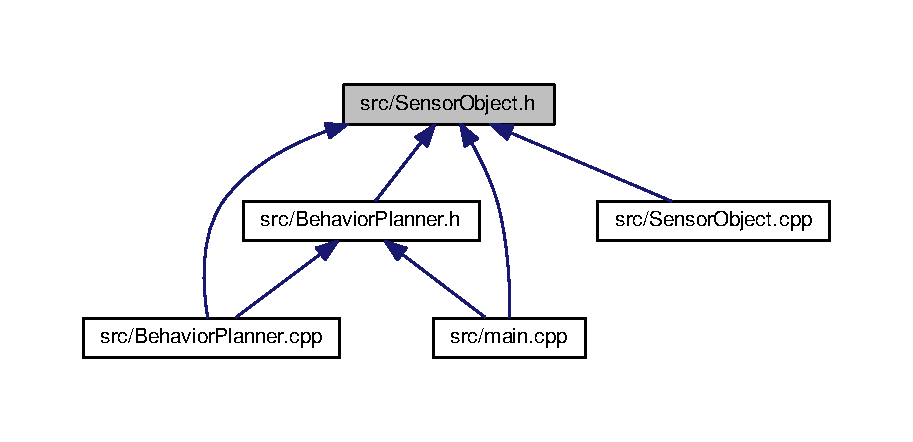
\includegraphics[width=350pt]{SensorObject_8h__dep__incl}
\end{center}
\end{figure}
\subsection*{Classes}
\begin{DoxyCompactItemize}
\item 
class \hyperlink{classSensorObject}{Sensor\+Object}
\end{DoxyCompactItemize}

\hypertarget{spline_8h}{}\section{src/spline.h File Reference}
\label{spline_8h}\index{src/spline.\+h@{src/spline.\+h}}
{\ttfamily \#include $<$cstdio$>$}\\*
{\ttfamily \#include $<$cassert$>$}\\*
{\ttfamily \#include $<$vector$>$}\\*
{\ttfamily \#include $<$algorithm$>$}\\*
Include dependency graph for spline.\+h\+:\nopagebreak
\begin{figure}[H]
\begin{center}
\leavevmode
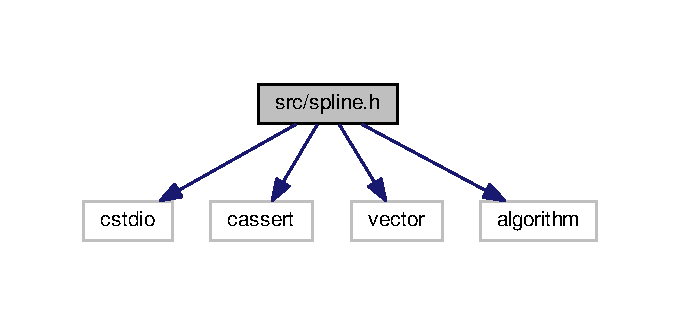
\includegraphics[width=327pt]{spline_8h__incl}
\end{center}
\end{figure}
This graph shows which files directly or indirectly include this file\+:\nopagebreak
\begin{figure}[H]
\begin{center}
\leavevmode
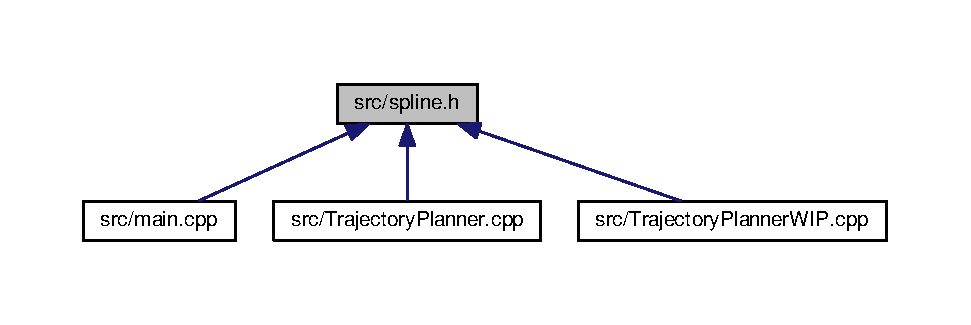
\includegraphics[width=350pt]{spline_8h__dep__incl}
\end{center}
\end{figure}
\subsection*{Namespaces}
\begin{DoxyCompactItemize}
\item 
 \hyperlink{namespacetk}{tk}
\end{DoxyCompactItemize}

\hypertarget{TrajectoryPlanner_8cpp}{}\section{src/\+Trajectory\+Planner.cpp File Reference}
\label{TrajectoryPlanner_8cpp}\index{src/\+Trajectory\+Planner.\+cpp@{src/\+Trajectory\+Planner.\+cpp}}
{\ttfamily \#include \char`\"{}Trajectory\+Planner.\+h\char`\"{}}\\*
{\ttfamily \#include \char`\"{}Ego\+Vehicle.\+h\char`\"{}}\\*
{\ttfamily \#include \char`\"{}helper.\+h\char`\"{}}\\*
{\ttfamily \#include \char`\"{}spline.\+h\char`\"{}}\\*
{\ttfamily \#include $<$fstream$>$}\\*
{\ttfamily \#include $<$iostream$>$}\\*
{\ttfamily \#include $<$math.\+h$>$}\\*
{\ttfamily \#include $<$vector$>$}\\*
{\ttfamily \#include $<$cmath$>$}\\*
{\ttfamily \#include \char`\"{}Dense\char`\"{}}\\*
Include dependency graph for Trajectory\+Planner.\+cpp\+:\nopagebreak
\begin{figure}[H]
\begin{center}
\leavevmode
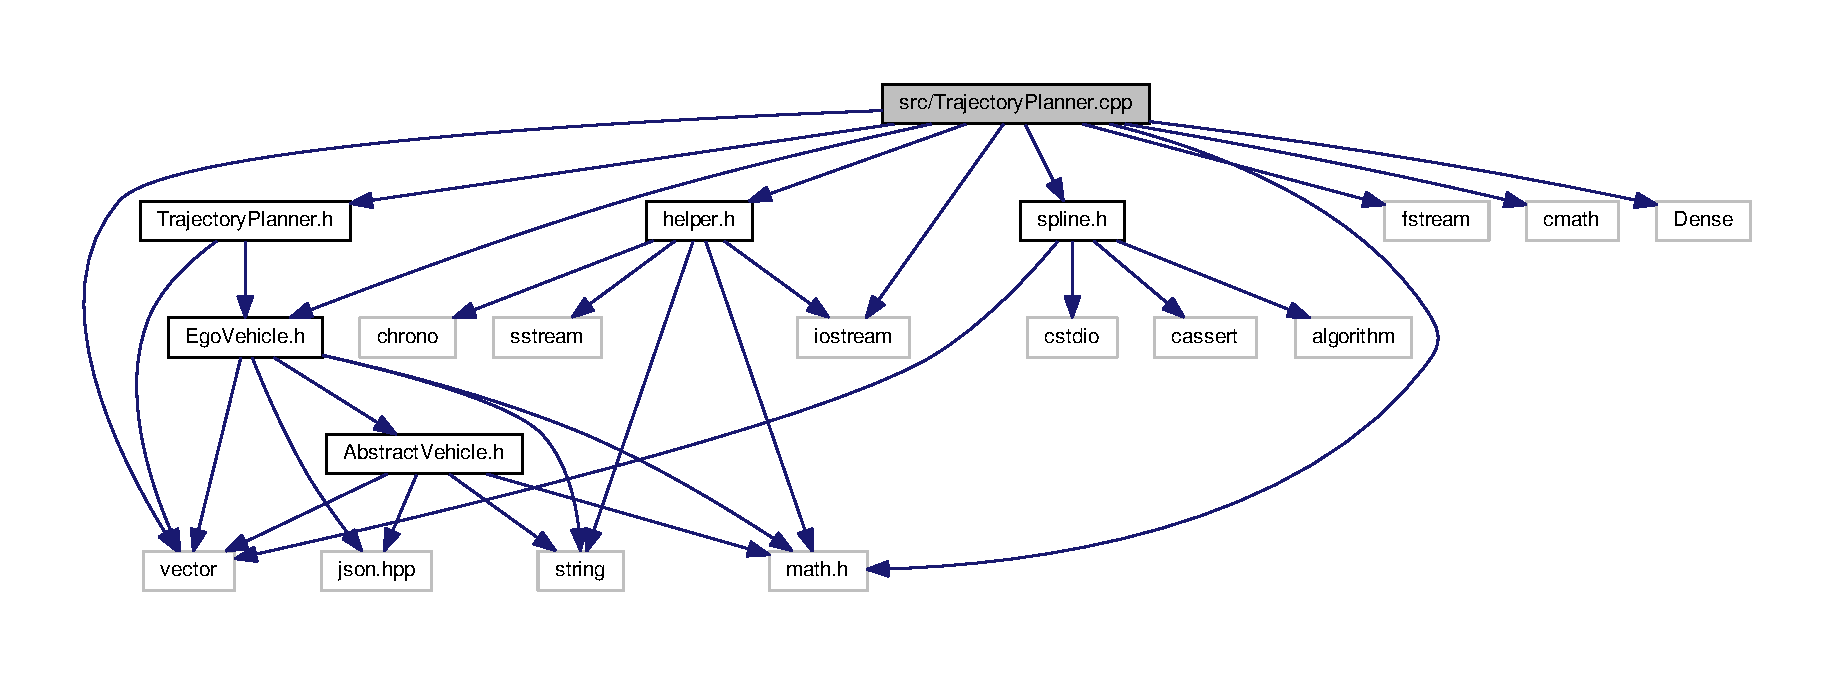
\includegraphics[width=350pt]{TrajectoryPlanner_8cpp__incl}
\end{center}
\end{figure}

\hypertarget{TrajectoryPlanner_8h}{}\section{src/\+Trajectory\+Planner.h File Reference}
\label{TrajectoryPlanner_8h}\index{src/\+Trajectory\+Planner.\+h@{src/\+Trajectory\+Planner.\+h}}
{\ttfamily \#include $<$vector$>$}\\*
{\ttfamily \#include \char`\"{}Ego\+Vehicle.\+h\char`\"{}}\\*
Include dependency graph for Trajectory\+Planner.\+h\+:\nopagebreak
\begin{figure}[H]
\begin{center}
\leavevmode
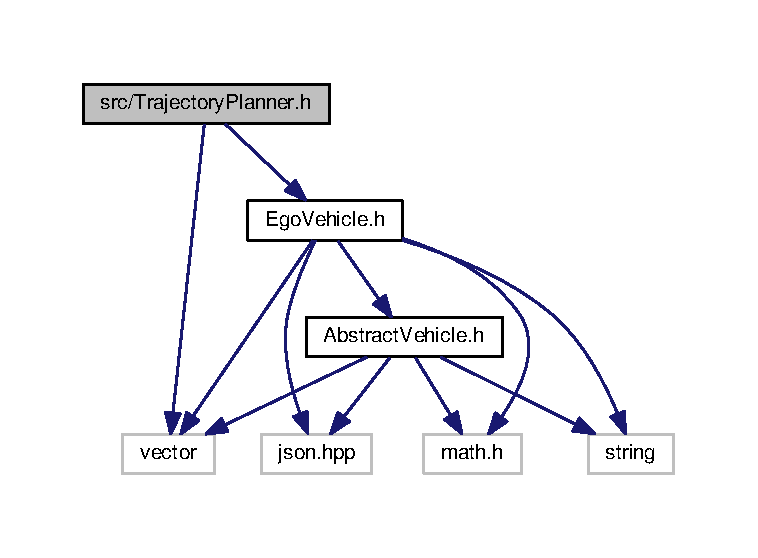
\includegraphics[width=350pt]{TrajectoryPlanner_8h__incl}
\end{center}
\end{figure}
This graph shows which files directly or indirectly include this file\+:\nopagebreak
\begin{figure}[H]
\begin{center}
\leavevmode
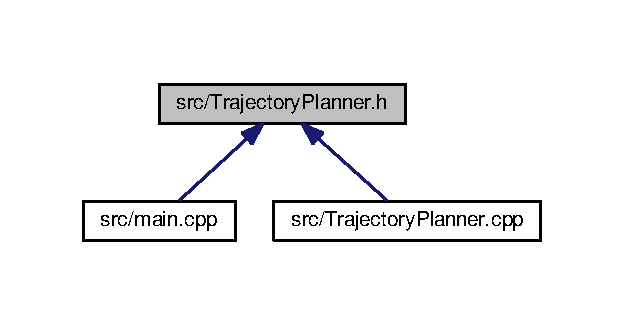
\includegraphics[width=300pt]{TrajectoryPlanner_8h__dep__incl}
\end{center}
\end{figure}
\subsection*{Classes}
\begin{DoxyCompactItemize}
\item 
class \hyperlink{classTrajectoryPlanner}{Trajectory\+Planner}
\end{DoxyCompactItemize}
\subsection*{Functions}
\begin{DoxyCompactItemize}
\item 
double \hyperlink{TrajectoryPlanner_8h_a19481c763d7a0b56b40eade0a21daab7}{pi} ()
\item 
double \hyperlink{TrajectoryPlanner_8h_adbcf4609758c05a6405c3d9c5f185e6b}{deg2rad} (double x)
\item 
double \hyperlink{TrajectoryPlanner_8h_aed6ee8bde39415298883a363b7759381}{rad2deg} (double x)
\item 
double \hyperlink{TrajectoryPlanner_8h_a7d653a23bc3022afd9b32e419abbbc2d}{distance} (double x1, double y1, double x2, double y2)
\end{DoxyCompactItemize}


\subsection{Function Documentation}
\index{Trajectory\+Planner.\+h@{Trajectory\+Planner.\+h}!deg2rad@{deg2rad}}
\index{deg2rad@{deg2rad}!Trajectory\+Planner.\+h@{Trajectory\+Planner.\+h}}
\subsubsection[{\texorpdfstring{deg2rad(double x)}{deg2rad(double x)}}]{\setlength{\rightskip}{0pt plus 5cm}double deg2rad (
\begin{DoxyParamCaption}
\item[{double}]{x}
\end{DoxyParamCaption}
)}\hypertarget{TrajectoryPlanner_8h_adbcf4609758c05a6405c3d9c5f185e6b}{}\label{TrajectoryPlanner_8h_adbcf4609758c05a6405c3d9c5f185e6b}
\index{Trajectory\+Planner.\+h@{Trajectory\+Planner.\+h}!distance@{distance}}
\index{distance@{distance}!Trajectory\+Planner.\+h@{Trajectory\+Planner.\+h}}
\subsubsection[{\texorpdfstring{distance(double x1, double y1, double x2, double y2)}{distance(double x1, double y1, double x2, double y2)}}]{\setlength{\rightskip}{0pt plus 5cm}double distance (
\begin{DoxyParamCaption}
\item[{double}]{x1, }
\item[{double}]{y1, }
\item[{double}]{x2, }
\item[{double}]{y2}
\end{DoxyParamCaption}
)}\hypertarget{TrajectoryPlanner_8h_a7d653a23bc3022afd9b32e419abbbc2d}{}\label{TrajectoryPlanner_8h_a7d653a23bc3022afd9b32e419abbbc2d}
\index{Trajectory\+Planner.\+h@{Trajectory\+Planner.\+h}!pi@{pi}}
\index{pi@{pi}!Trajectory\+Planner.\+h@{Trajectory\+Planner.\+h}}
\subsubsection[{\texorpdfstring{pi()}{pi()}}]{\setlength{\rightskip}{0pt plus 5cm}double pi (
\begin{DoxyParamCaption}
{}
\end{DoxyParamCaption}
)}\hypertarget{TrajectoryPlanner_8h_a19481c763d7a0b56b40eade0a21daab7}{}\label{TrajectoryPlanner_8h_a19481c763d7a0b56b40eade0a21daab7}
\index{Trajectory\+Planner.\+h@{Trajectory\+Planner.\+h}!rad2deg@{rad2deg}}
\index{rad2deg@{rad2deg}!Trajectory\+Planner.\+h@{Trajectory\+Planner.\+h}}
\subsubsection[{\texorpdfstring{rad2deg(double x)}{rad2deg(double x)}}]{\setlength{\rightskip}{0pt plus 5cm}double rad2deg (
\begin{DoxyParamCaption}
\item[{double}]{x}
\end{DoxyParamCaption}
)}\hypertarget{TrajectoryPlanner_8h_aed6ee8bde39415298883a363b7759381}{}\label{TrajectoryPlanner_8h_aed6ee8bde39415298883a363b7759381}

\hypertarget{TrajectoryPlannerWIP_8cpp}{}\section{src/\+Trajectory\+Planner\+W\+IP.cpp File Reference}
\label{TrajectoryPlannerWIP_8cpp}\index{src/\+Trajectory\+Planner\+W\+I\+P.\+cpp@{src/\+Trajectory\+Planner\+W\+I\+P.\+cpp}}
{\ttfamily \#include \char`\"{}Trajectory\+Planner\+W\+I\+P.\+h\char`\"{}}\\*
{\ttfamily \#include \char`\"{}Ego\+Vehicle.\+h\char`\"{}}\\*
{\ttfamily \#include \char`\"{}helper.\+h\char`\"{}}\\*
{\ttfamily \#include \char`\"{}spline.\+h\char`\"{}}\\*
{\ttfamily \#include $<$fstream$>$}\\*
{\ttfamily \#include $<$iostream$>$}\\*
{\ttfamily \#include $<$math.\+h$>$}\\*
{\ttfamily \#include $<$vector$>$}\\*
{\ttfamily \#include $<$cmath$>$}\\*
{\ttfamily \#include \char`\"{}Dense\char`\"{}}\\*
Include dependency graph for Trajectory\+Planner\+W\+I\+P.\+cpp\+:\nopagebreak
\begin{figure}[H]
\begin{center}
\leavevmode
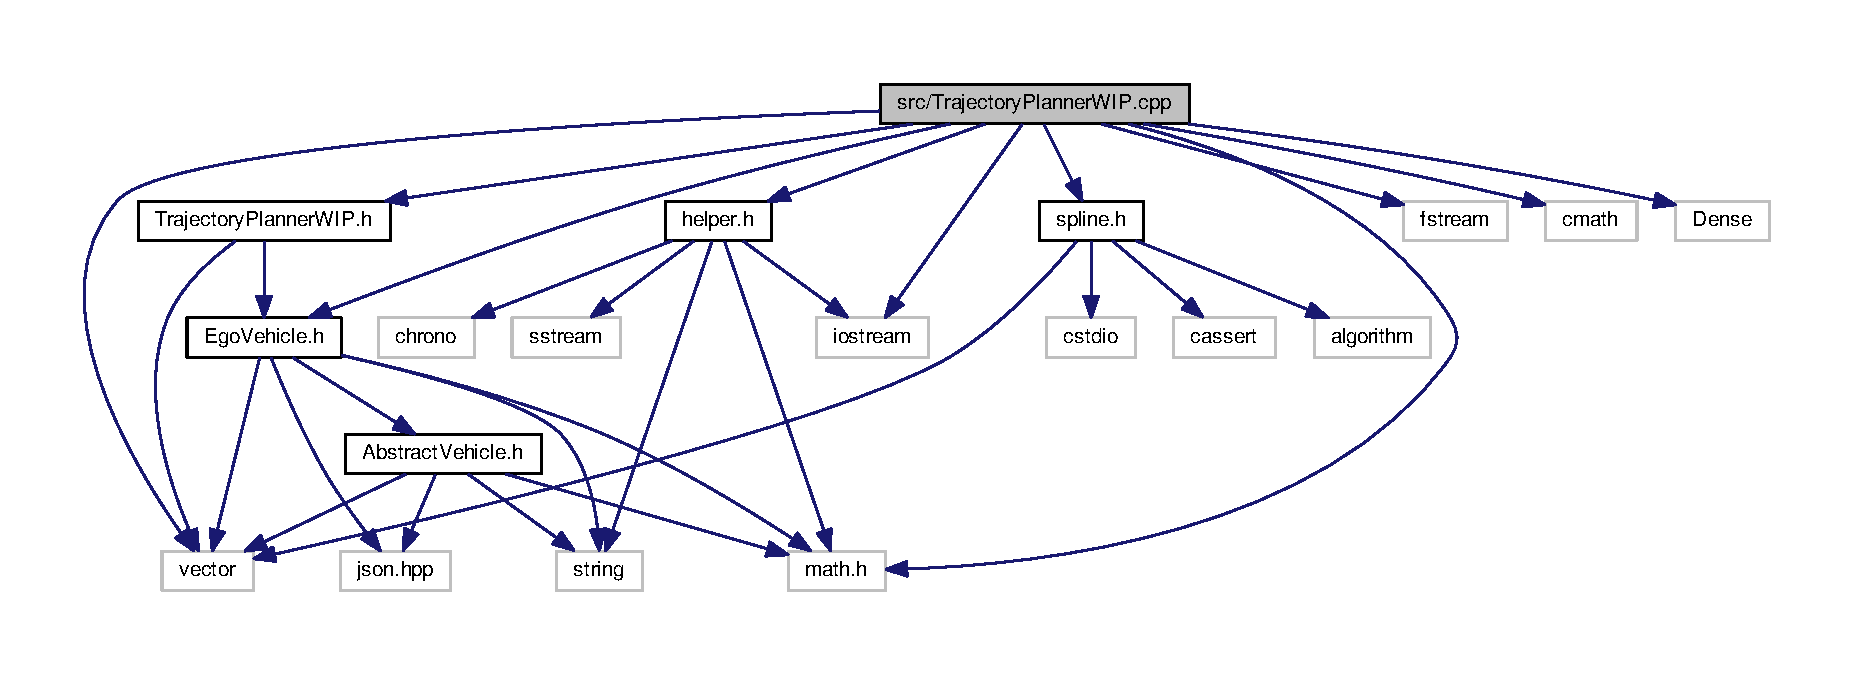
\includegraphics[width=350pt]{TrajectoryPlannerWIP_8cpp__incl}
\end{center}
\end{figure}

\hypertarget{TrajectoryPlannerWIP_8h}{}\section{src/\+Trajectory\+Planner\+W\+IP.h File Reference}
\label{TrajectoryPlannerWIP_8h}\index{src/\+Trajectory\+Planner\+W\+I\+P.\+h@{src/\+Trajectory\+Planner\+W\+I\+P.\+h}}
{\ttfamily \#include $<$vector$>$}\\*
{\ttfamily \#include \char`\"{}Ego\+Vehicle.\+h\char`\"{}}\\*
Include dependency graph for Trajectory\+Planner\+W\+I\+P.\+h\+:\nopagebreak
\begin{figure}[H]
\begin{center}
\leavevmode
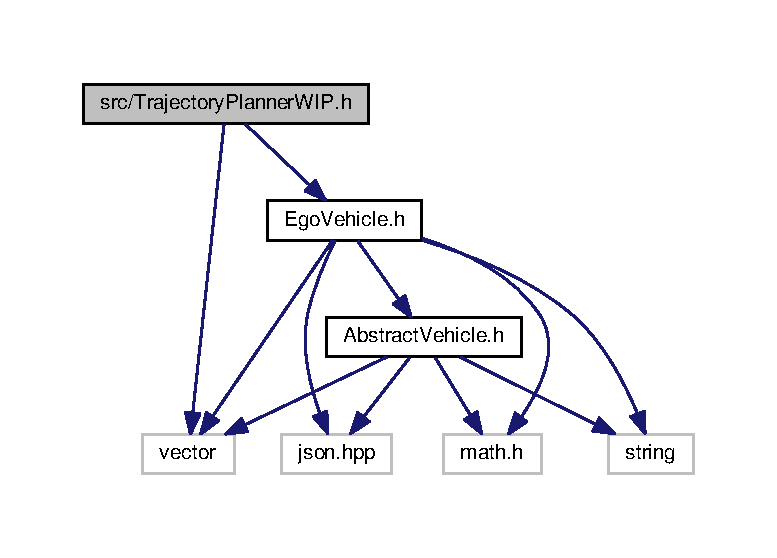
\includegraphics[width=350pt]{TrajectoryPlannerWIP_8h__incl}
\end{center}
\end{figure}
This graph shows which files directly or indirectly include this file\+:\nopagebreak
\begin{figure}[H]
\begin{center}
\leavevmode
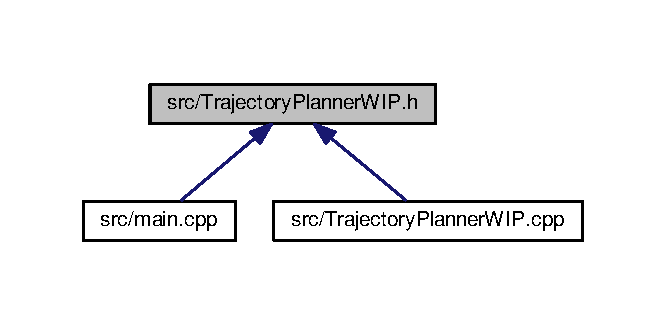
\includegraphics[width=320pt]{TrajectoryPlannerWIP_8h__dep__incl}
\end{center}
\end{figure}
\subsection*{Classes}
\begin{DoxyCompactItemize}
\item 
class \hyperlink{classTrajectoryPlannerWIP}{Trajectory\+Planner\+W\+IP}
\end{DoxyCompactItemize}
\subsection*{Functions}
\begin{DoxyCompactItemize}
\item 
double \hyperlink{TrajectoryPlannerWIP_8h_a19481c763d7a0b56b40eade0a21daab7}{pi} ()
\item 
double \hyperlink{TrajectoryPlannerWIP_8h_adbcf4609758c05a6405c3d9c5f185e6b}{deg2rad} (double x)
\item 
double \hyperlink{TrajectoryPlannerWIP_8h_aed6ee8bde39415298883a363b7759381}{rad2deg} (double x)
\item 
double \hyperlink{TrajectoryPlannerWIP_8h_a7d653a23bc3022afd9b32e419abbbc2d}{distance} (double x1, double y1, double x2, double y2)
\end{DoxyCompactItemize}


\subsection{Function Documentation}
\index{Trajectory\+Planner\+W\+I\+P.\+h@{Trajectory\+Planner\+W\+I\+P.\+h}!deg2rad@{deg2rad}}
\index{deg2rad@{deg2rad}!Trajectory\+Planner\+W\+I\+P.\+h@{Trajectory\+Planner\+W\+I\+P.\+h}}
\subsubsection[{\texorpdfstring{deg2rad(double x)}{deg2rad(double x)}}]{\setlength{\rightskip}{0pt plus 5cm}double deg2rad (
\begin{DoxyParamCaption}
\item[{double}]{x}
\end{DoxyParamCaption}
)}\hypertarget{TrajectoryPlannerWIP_8h_adbcf4609758c05a6405c3d9c5f185e6b}{}\label{TrajectoryPlannerWIP_8h_adbcf4609758c05a6405c3d9c5f185e6b}


Here is the call graph for this function\+:\nopagebreak
\begin{figure}[H]
\begin{center}
\leavevmode
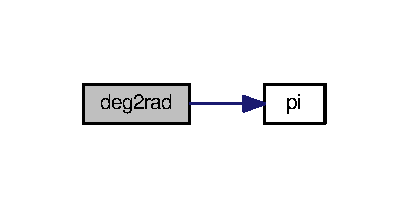
\includegraphics[width=196pt]{TrajectoryPlannerWIP_8h_adbcf4609758c05a6405c3d9c5f185e6b_cgraph}
\end{center}
\end{figure}


\index{Trajectory\+Planner\+W\+I\+P.\+h@{Trajectory\+Planner\+W\+I\+P.\+h}!distance@{distance}}
\index{distance@{distance}!Trajectory\+Planner\+W\+I\+P.\+h@{Trajectory\+Planner\+W\+I\+P.\+h}}
\subsubsection[{\texorpdfstring{distance(double x1, double y1, double x2, double y2)}{distance(double x1, double y1, double x2, double y2)}}]{\setlength{\rightskip}{0pt plus 5cm}double distance (
\begin{DoxyParamCaption}
\item[{double}]{x1, }
\item[{double}]{y1, }
\item[{double}]{x2, }
\item[{double}]{y2}
\end{DoxyParamCaption}
)}\hypertarget{TrajectoryPlannerWIP_8h_a7d653a23bc3022afd9b32e419abbbc2d}{}\label{TrajectoryPlannerWIP_8h_a7d653a23bc3022afd9b32e419abbbc2d}
\index{Trajectory\+Planner\+W\+I\+P.\+h@{Trajectory\+Planner\+W\+I\+P.\+h}!pi@{pi}}
\index{pi@{pi}!Trajectory\+Planner\+W\+I\+P.\+h@{Trajectory\+Planner\+W\+I\+P.\+h}}
\subsubsection[{\texorpdfstring{pi()}{pi()}}]{\setlength{\rightskip}{0pt plus 5cm}double pi (
\begin{DoxyParamCaption}
{}
\end{DoxyParamCaption}
)}\hypertarget{TrajectoryPlannerWIP_8h_a19481c763d7a0b56b40eade0a21daab7}{}\label{TrajectoryPlannerWIP_8h_a19481c763d7a0b56b40eade0a21daab7}
\index{Trajectory\+Planner\+W\+I\+P.\+h@{Trajectory\+Planner\+W\+I\+P.\+h}!rad2deg@{rad2deg}}
\index{rad2deg@{rad2deg}!Trajectory\+Planner\+W\+I\+P.\+h@{Trajectory\+Planner\+W\+I\+P.\+h}}
\subsubsection[{\texorpdfstring{rad2deg(double x)}{rad2deg(double x)}}]{\setlength{\rightskip}{0pt plus 5cm}double rad2deg (
\begin{DoxyParamCaption}
\item[{double}]{x}
\end{DoxyParamCaption}
)}\hypertarget{TrajectoryPlannerWIP_8h_aed6ee8bde39415298883a363b7759381}{}\label{TrajectoryPlannerWIP_8h_aed6ee8bde39415298883a363b7759381}


Here is the call graph for this function\+:\nopagebreak
\begin{figure}[H]
\begin{center}
\leavevmode
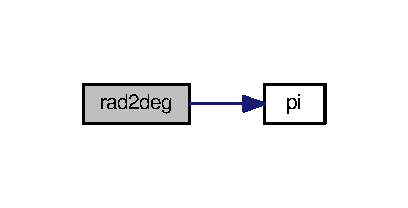
\includegraphics[width=196pt]{TrajectoryPlannerWIP_8h_aed6ee8bde39415298883a363b7759381_cgraph}
\end{center}
\end{figure}



%--- End generated contents ---

% Index
\backmatter
\newpage
\phantomsection
\clearemptydoublepage
\addcontentsline{toc}{chapter}{Index}
\printindex

\end{document}
